\documentclass[9pt,a4paper]{book}
%
\usepackage{amsmath}
\usepackage[latin2]{inputenc}
\usepackage{graphicx}
\usepackage[magyar]{babel}
\usepackage{t1enc}
%\usepackage[bookmarksopen=true]{hyperref}
\usepackage{color}
\usepackage{floatflt}
\usepackage{lmodern}
\usepackage{ulem}
\usepackage{fancyhdr}
%
\setlength{\topmargin}{-0.5in}
\setlength{\textheight}{9in}
\setlength{\oddsidemargin}{-0.1in}
\setlength{\evensidemargin}{0.in}
\setlength{\textwidth}{6.5in}
\setlength{\headsep}{1.2cm}
\setlength{\parskip}{0.4cm}
\setlength{\parindent}{0.cm}
\setcounter{tocdepth}{4}
\setcounter{secnumdepth}{4}
%

%\pagestyle{headings}
 
\title{Tranziens szimul�tor hidraulikai rendszerekhez}
\author{\copyright H�s Csaba\\ B�rdossy Gergely, Heged�s Ferenc, Pandula Zolt�n, Moln�r Gerg�\\
BME Hidrodinamikai Rendszerek Tansz�k}

%%%%%%%%%%%%%%%%%%%%%%%%%%%%%%%%%%%%%%%%%%%%%%%%%%%%%%%%%%%%%%%%%%%%%%%%%

\begin{document}
\nocite{fuzy}
\pagestyle{empty}

\maketitle
\clearpage{\pagestyle{empty}\cleardoublepage}
\tableofcontents
\listoffigures
\clearpage{\pagestyle{empty}\cleardoublepage}

\pagestyle{fancy}

\chapter{A sz�m�t�si m�dszer}

\section{El�zm�nyek}

\section{Rugalmas cs�vek}

\begin{eqnarray}
\text{A $\mathcal{C}^+$ karakterisztika ment�n:} & \frac{d}{dt} \left( p+\rho a v\right) &= \mathcal{S}^+=-\rho g a \frac{dz}{dx} - \frac{\lambda}{2 D} \rho a v \left| v \right| \label{eq:karp}\\
\text{A $\mathcal{C}^-$ karakterisztika ment�n:} & \frac{d}{dt} \left( p-\rho a v\right) &= \mathcal{S}^-=\rho g a \frac{dz}{dx} + \frac{\lambda}{2 D} \rho a v \left| v \right| \label{eq:karm}
\end{eqnarray}

\section{Merev alrendszerek}

A merev alrendszer tetsz�leges bonyolults�g� - csom�pontokat �s �.n. �gakat tartalmaz�, hurkolt - h�l�zat r�sz, amelynek n�h�ny �ga csatlakozik egy-egy rugalmas cs�h�z. Az ilyen h�l�zat r�szeket - amelyekben a t�vols�gok a rugalmas cs�vek hossz�hoz k�pest kicsik, ez�rt a tranziens v�ltoz�sok a h�l�zat r�sz minden pontj�n gyakorlatilag egyidej�leg k�vetkeznek be - merev alrendszereknek nevezz�k.

A merev alrendszerek modellje a csom�ponti kontinuit�s �s az �gegyenletek. Ha $j$-edik csom�pontba $K$ darab �g fut be, az �gak ${\dot m}_k$ t�meg�ramainak el�jeles �sszege megegyezik a csom�ponti fogyaszt�ssal (�gak eset�n a csom�pontba �rkez� t�meg�ramot tekintj�k pozit�vnak, m�g fogyaszt�sok eset�n az elv�telt):
%
\begin{equation}
\sum_{k=1}^K {\dot m}_k = f_j.
\label{eq:konti}
\end{equation}
%
Az �gat �raml�stanilag az �gegyenlet jellemzi, amely az �g t�meg�ram�nak legfeljebb m�sodfok� polinomja id�ben �lland�, illetve v�ltoz� egy�tthat�kkal:
%
\begin{equation}
\alpha\, \dot m + \beta\, {\dot m}^2 + \gamma \dot m\,\left| \dot m \right| + \delta + p_e-p_v=0,
\label{eq:egyenlet}
\end{equation}
%
ahol az �g elej�t - tetsz�legesen r�gz�tett �raml�si ir�nnyal defini�lva - $e$, v�g�t $v$ jel�li, $p$ pedig a nyom�s a megfelel� pontokban.

K�l�n megeml�tj�k a rugalmas cs�vekhez val� csatlakoz�si pontokat. Az \eqref{eq:karp} �s \eqref{eq:karm} karakterisztika egyenletek seg�ts�g�vel �rhatjuk, hogy 
%
\begin{equation}
p \pm \frac{a }{A} {\dot m}_r - \left( \tilde p \pm \rho a \tilde v \right)-\Delta t \,\mathcal{S}^\pm=0,
\end{equation}
%
ahol $p$ a merev alrendszerhez tartoz� (csatlakoz�) csom�pont nyom�s�t jel�li, ${\dot m}_r$ a rugalmas cs�beli t�meg�ramot, $\tilde p$ �s $\tilde v$ a cs�beli \emph{szomsz�dos} oszt�spontbeli nyom�st �s sebess�get jel�li.

Egy adott merev alrendszerben ismeretlen mennyis�gek az �g�ramok ($n_{ag}$ darab) �s a csom�ponti nyom�sok ($n_{csp}$ db), ezen k�v�l az egyes kapcsol�d� rugalmas cs�vek t�meg�ramai a csatlakoz� pontban ($n_{rug}$ darab). E mennyis�gek meghat�roz�s�hoz rendelkez�s�nkre �llnak az \eqref{eq:egyenlet} alak� �gegyenletek, minden csom�pontban a \eqref{eq:konti} kontinuit�si egyenlet �s minden kapcsol�d� rugalmas cs� eset�n egy-egy karakterisztika egyenlet; \ref{eq:karp} $\mathcal{C}^+$ ment�n (a cs� v�ge csatlakozik a merev alrendszerhez) vagy \eqref{eq:karm} $\mathcal{C}^-$ ment�n (a cs� eleje csatlakozik a merev alrendszerhez), azaz pontosan annyi egyenlet �ll rendelkez�s�nkre, mint ah�ny ismeretlen mennyis�g.

A hagyom�nyos sz�m�t�si m�dszer (ld. p�ld�ul Hal�sz �s szerz�t�rsai, 2002) �n. b�zis�ram kiv�laszt�ssal indul, mely a merev alrendszer gr�fj�ban f�ggetlen hurkokat �ll�t el� �s kik�sz�b�li az ismeretlen nyom�sokat. A b�zis�ramok meghat�rozhat�k, majd egyszer� visszahelyettes�t�ssel a t�bbi �g�ram �s a nyom�sok is sz�m�that�k. Mivel �ltal�ban a b�zis�ramok sz�ma sokkal kevesebb, mint az �g�ramok sz�ma, a feladat m�rete jelent�sen cs�kken, ami gyors�tja a megold�st. B�r a b�zis�ram kiv�laszt�son alapul� m�dszer hat�kony (gyors) �s az elm�lt �vtizedek tapasztalata szerint stabil �s mentes a numerikus oszcill�ci�kt�l, h�tr�nya, hogy programoz�sa bonyolult. Az al�bbiakban e kifinomult m�dszerrel szemben egy �ltal�nos c�l� megold�t mutatunk be, mely ugyan kev�sb� hat�kony, de igen k�nnyen programozhat� �s a kereskedelmi forgalomban kaphat� PC-k sebess�g�t figyelembe v�ve nem okoz elviselhetetlen�l nagyobb megterhel�st a sz�m�t�g�pnek.

Els� l�p�sk�nt foglaljuk �ssze a merev alrendszer ismeretlen mennyis�geit egy vektorba:
%
\begin{equation}
\mathbf{x}=\left({\dot m}_1,{\dot m}_2,\dots,{\dot m}_i,\dots,{\dot m}_{n_{ag}},\, p_1,p_2,\dots,p_j,\dots,p_{n_{csp}},r_1,r_2,\dots,r_k,\dots,r_{n_{rug}} \right)^T,
\end{equation}
%
ahol $r_i$ a rugalmas cs�vek t�meg�ram�t jel�li.

\emph{ide m�g duma...}

A megoldand� egyenletrendszer teh�t
%
\begin{equation}
\mathbf{f(x)}=
\begin{pmatrix} [\alpha_i] & \mathbf{\Pi} & \mathbf{0}\\ \mathbf{K} & \mathbf{0} & \mathbf{P} \\ \mathbf{0} & \mathbf{E} & [\alpha_k] \end{pmatrix}\, \mathbf{x} \,+\,
\begin{pmatrix} [\beta_i] & \mathbf{0} & \mathbf{0}\\ \mathbf{0} & \mathbf{0} & \mathbf{0} \\ \mathbf{0} & \mathbf{0} & \mathbf{0} \end{pmatrix}\, \mathbf{x}^2 \,+\,
\begin{pmatrix} [\gamma_i] & \mathbf{0} & \mathbf{0}\\ \mathbf{0} & \mathbf{0} & \mathbf{0} \\ \mathbf{0} & \mathbf{0} & \mathbf{0} \end{pmatrix}\, \mathbf{x} \left|\mathbf{x} \right|  \,+\,
\begin{pmatrix} \delta_i \\ f_j \\ -\Delta t\, \mathcal{S}_k^\pm \end{pmatrix} \,= \, \mathbf{0},
\end{equation}
%
ahol a $[\dots]$ jel�l�s diagon�l m�trixot jel�l. A vastagon szedett m�trixok csak $\pm1$-et vagy $0$ elemeket tartalmaznak, pl. a $\mathbf{\Pi}$ m�trix $i$-edik sor�nak $j$-edik eleme $1$, ha az $i$-edik �gelem a $j$-edik csom�pontba fut be, $-1$, ha onnan indul, egy�bk�nt 0. Hasonl�an, a $\mathbf{K}$ m�trix j-edik sor�nak $i$-edik oszlopa $1$, ha az $i$-edik �gelem belefut a $j$-edik csom�pontba, $-1$ ha onnan indul, egy�bk�nt z�rus. A $\mathbf{P}$ m�trix $j$-edik sor�nak $k$-adik eleme $1$, ha ebbe a $j$-edik csom�pontba a $k$-adik rugalmas cs� befut, $-1$, ha onnan indul �s egy�bk�nt z�rus. V�g�l, az $\mathbf{E}$ m�trix $k$-adik sor�nak $j$-edik elem $1$, ha a $k$-adik rugalmas cs� a $j$-edik csom�pontba csatlakozik, egy�bk�nt z�rus.

%%%%%%%%%%%%%%%%%%%%%%%%%%%%%%%%%%%%%%%%%%%%%%%%%%%%%%%%%%%%%5

\section{�gegyenletek}

\subsection{Cs�}

A legtipikusabb �g a cs�, melynek keresztmetszete $A$, �tm�r�je $d$, hossza $L$, $h_e$ �s $h_v$ az elej�nek �s v�g�nek magass�ga, m�g $p_e$ �s $p_v$ a nyom�st jel�li a cs� elej�n �s v�g�n. A cs�ben foly� t�meg�ram $\dot m$. Kiindul�sk�nt �rjuk fel az instacioner Bernoulli egyenletet:
%
\begin{equation}
p_e + \frac{\rho}{2}v_e^2 + \rho\,g\,h_e =p_v + \frac{\rho}{2}v_v^2 + \rho\,g\,h_v + \lambda \frac{L}{D}\frac{\rho}{2}\,v\,\left| v \right| + \rho\,L \frac{dv}{dt}.
\label{eq:cso_agegyenlet}
\end{equation}
%
Mivel a keresztmetszet �lland�, $v_e=v_v=v=\dot m/(\rho A)$. A sebess�g deriv�ltj�t �rjuk
%
\begin{equation}
\frac{dv}{dt}=\frac{1}{\rho A}\frac{\dot m - {\dot m}_r}{\Delta t}
\end{equation}
%
alakban, ahol $v_r$ az el�z� id�szinten vett sebess�g. �gy \eqref{eq:cso_agegyenlet} az al�bbi alakot �lti.
%
\begin{equation}
0=p_v-p_e + \rho\,g\,\left(h_v-h_e \right) + \lambda \frac{L}{\rho 2 D A^2}\,\dot m\,\left| \dot m \right| + \frac{L}{A \Delta t} \left( \dot m - {\dot m}_r \right),
\end{equation}
%
amelyb�l kiolvashatjuk az �gegyenlet egy�tthat�it:
%
\begin{equation}
\alpha=\frac{L}{A \Delta t}, \quad \beta=0, \quad \gamma=\lambda \frac{L}{\rho 2 D A^2}\quad \text{�s} \quad \delta=  \rho\,g\,\left(h_v-h_e \right) - \frac{L}{A \Delta t}{\dot m}_r.
\end{equation}

%%%%%%%%%%%%%%%%%%%%%%%%%%%%%%%%%%%%%%%%%%%%%%%%%%%%%%%%%%%%%%%%%%%%%%%%%
\subsection{L�g�st}

A politropikus �llapotv�ltoz�st v�gz� l�g�st modellje a \ref{legust}. �br�n l�that�. \fbox{Ide m�g egy csom� sz�veg j�n.} A l�g�st keresztmetszete $A$, magass�ga $H$, a folyad�kfelsz�n felett elhelyezked� l�gp�rna nyom�sa $p$, t�rfogata $V$. A l�g�st�t agy $l$ hossz�s�g� f�gg�leges cs� k�ti a rendszerhez. A l�g�st talppontj�ban a nyom�s $p_t$ �s $Q$ t�rfogat�ram �ramlik a l�g�st\emph{be}. 
%
\begin{figure}[h]
  \begin{center}
    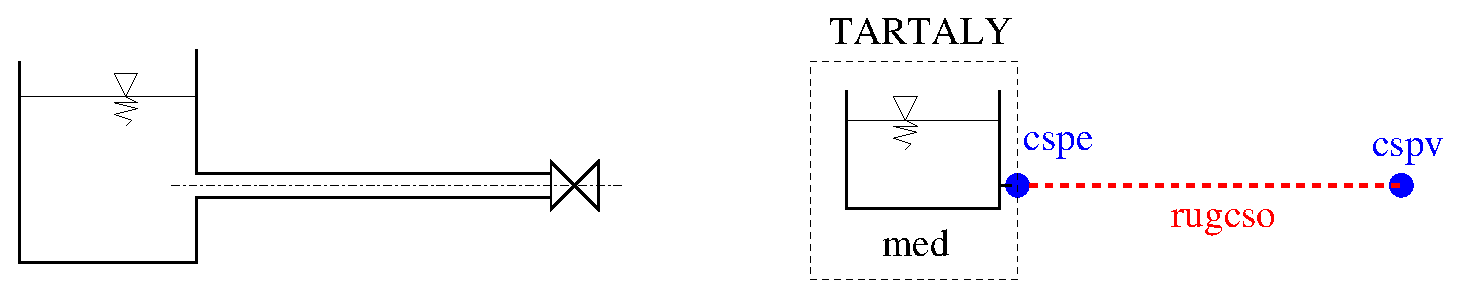
\includegraphics[width=15cm]{abrak/feladat1abra.eps}
    \caption{\label{legust}L�g�st modell}
  \end{center}
\end{figure}

A talpponti nyom�s a l�gp�rna nyom�s�nak �s a folyad�koszlop hidrosztatikus nyom�s�nak �sszege:
%
\begin{equation}
p_t = p+\rho\,g\,\left( l+H-\frac{V}{A}\right).
\label{eq:legust1}
\end{equation}
% 
Mivel a l�gp�rna �llapotv�ltoz�sa politropikus, �gy $p\,V^n=konst.$, ez�rt
%
\begin{equation}
0=\frac{d\,\left( p\,V^n \right)}{dt}=V^n \frac{dp}{dt}+nV^{n-1}p \frac{dV}{dt} \quad \rightarrow \quad \frac{dp}{dt} = -n\frac{p}{V}\frac{dV}{dt}=n\frac{p}{V}Q,
\end{equation}
%
melyet $\Delta t$ l�p�sre integr�lva kapjuk, hogy ($p^i=p(t)$, $p^{i+1}=p(t+\Delta t)$)
%
\begin{equation}
p^{i+1}-p^i=\Delta t\, Q\, n \left( \frac{\overline{p}}{\overline{V}}\right),
\end{equation}
%
ahol a fel�lvon�sos �rt�kek az inter�l�si tartom�nyon vett �tlag�rt�ket jelentik. Ezt pl. extrapol�ci�val sz�m�thatjuk ki az el�z� k�t �rt�kb�l. �rjuk fel az \eqref{eq:legust1} hidrosztatikai egyenletet a sz�m�tand� �s az el�z� id�l�p�sre:
%
\begin{eqnarray}
p_t^{i+1} &= p^{i+1} + \rho\,g\,\left( l+H-\frac{V^{i+1}}{A}\right),
p_t^{i}   &= p^{i  } + \rho\,g\,\left( l+H-\frac{V^{i}}{A}\right),
\end{eqnarray}
%
�s vegy�k a kett� k�l�nbs�g�t:
%
\begin{equation}
p_t^{i+1} - p_t^{i} = p^{i+1} -p^{i} - \rho\,g\,\left( \frac{V^{i+1}-V^i}{A}\right) \approx p^{i+1} -p^{i} - \frac{\rho\,g}{A}\,\Delta t\,Q =
\Delta t\, Q\, \left[ n \left( \frac{\overline{p}}{\overline{V}}\right) - \frac{\rho\,g}{A} \right].
\end{equation}
%
Teh�t az �gegyenlet egy�tthat�i:
%
\begin{equation}
\alpha=\Delta t\, \left[ n \left( \frac{\overline{p}}{\overline{V}}\right) - \frac{\rho\,g}{A} \right], \quad \delta = -p_t^{i} \quad \text{�s} \quad \beta=\gamma=0.
\end{equation}
\clearpage{\pagestyle{empty}\cleardoublepage}
\chapter{Szimul�ci�}

\section{Adat el�k�sz�t�s}

A tranziens h�l�zatsz�m�t�s els� l�p�se - hasonl�an az �lland�sult �llapotbeli vizsg�lathoz - a vizsg�lt rendszer hidraulikai modellj�nek elk�sz�t�se. Ezut�n elk�sz�tj�k a merev alrendszerek kapcsol�si rajz�t, amely tartalmaz minden olyan elemet, mely a rendszer viselked�s�t �rdemlegesen befoly�solja. Ez a kapcsol�si rajz nem felt�tlen�l egyezik a stacioner h�l�zatsz�m�t�s kapcsol�si rajz�val, ugyanis pl. egy visszacsap� szelep vagy egy vez�relt/szab�lyozott elem a stacioner m�k�d�s szempontj�b�l ugyan k�z�mb�s, de tranziens folyamatok eset�n igen fontos szerepe lehet. Az egyes elemek csom�pontokban kapcsol�dnak egym�shoz. Az �gelemeket �s a csom�pontokat egyedi n�vvel l�tjuk el. A vizsg�lt rendszerben (az �sszes merev alrendszert �s az �sszes rugalmas cs�vet bele�rtve) {\bf minden csom�pontnak �s �gelemnek k�l�nb�z� neve legyen}! V�g�l �sszegy�jtj�k az �gelemek jellemz�it �s meg�rjuk az adatf�jlt (a k�s�bbiekben taglalt szintaktika szerint). Az adatokat egyetlen adatf�jlban foglaljuk �ssze, amelynek .tpr (tranziens projekt) nevet javasoljuk (de ez nem k�telez�).

\section{R�gi �s �j adatstrukt�r�k �s f�jlok}

2010 janu�rj�ban a le�r� adat�llom�nyokat egyszer�s�tett�k. Ez a dokument�ci� m�r csak az �j adatstrukt�r�kat le�r�s�t tartalmazza.

A r�gi adatstrukt�r�kat a k�vetkez� f�ggv�nyek t�mogatj�k: 
\begin{itemize}
\item {\tt trsz\_old.m (olvas\_merev\_old.m, olvas\_rugalmas\_old.m)}
\item {\tt trsz\_rajz\_old.m}
\end{itemize}

\clearpage

\section{A program haszn�lata}

\subsection{Sz�m�t�s}

A sz�m�t�s maga {\tt Matlab} k�rnyezetben a
%
\begin{verbatim}
>> trsz(<adatfajl>,<tmax>)
\end{verbatim}
%
parancs megh�v�s�val t�rt�nik. Az els� param�ter az adatf�jl neve kiterjeszt�ssel (pl.{\tt 'feladat.tpr'}), a m�sodik param�ter a szimul�ci� id�tartama m�sodpercben (pl. {\tt 60}).

Aj�nlott minden futtat�st k�l�n k�nyvt�rban v�gezni az adat-, ill. az eredm�nyf�jlok kevered�s�nek elker�l�se v�gett. A szimul�ci� sor�n az al�bbi f�jlok keletkeznek: 
\begin{itemize}
\item Minden merev alrendszerhez egy-egy {\tt <nev>.out} �s {\tt <nev>.res} �llom�ny. Az el�bbi k�zvetlen�l olvashat� sz�veges �llom�ny, az ut�bbi csak a sz�m�t�s numerikus eredm�nyeit tartalmazza, �rtelmez�s�hez a {\tt trsz\_rajz.m} eredm�nymegjelen�t� program sz�ks�ges. Az {\tt .out} f�jl r�szletess�g�t a {\tt mar\_debug\_level} opci�val lehet be�ll�tani az adatf�jlban \fbox{TODO}.
\item A rugalmas cs�vekben lezajl� folyamatokat (cs�venk�nt) egy-egy {\tt <nev>.res} �llom�ny tartalmazza, melyet ugyancsak az eredm�nymegjelen�t� program olvas.
\end{itemize}

A megold� h�v�sakor lehet�s�g van tov�bbi opci�k megad�s�ra:
%
\begin{verbatim}
>> trsz(<adatfajl>,<tmax>,<option1>,<ertek1>,<option2>,<ertek2>,...),
\end{verbatim}
%
melyek lehets�ges �rt�kei:

\begin{center}
\begin{tabular}{l|c|p{12cm}}
option      & t�pus   & �rt�k \\ \hline \hline 
{\tt debug} & integer & 0,1,2,3,4,5: debug szint, az emelked� �rt�kekhez egyre r�szletesebb kimenet tartozik\\\hline 
{\tt t0}    & double  & kezdeti id�pont megad�sa\\\hline 
{\tt dtmin} & double  & minim�lis id�l�p�s (a merev alrendszerek friss�t�s�re)\\\hline 
\end{tabular}
\end{center}

\subsection{Eredm�nyek megjelen�t�se}

A sz�m�t�sok eredm�nyeit a {\tt trsz\_rajz} programmal tekinthetj�k meg, ennek szintaktik�ja t�bbf�le lehet.

\subsection{Egyszer� rajz}

\begin{verbatim}
>> trsz_rajz('fnev','hol1','hol2','mit')
\end{verbatim}

Az els� argumentum a feladatot tartalmaz� adatf�jl neve kiterjeszt�ssel. A {\tt hol1} adat lehet merev alrendszer vagy rugalmas cs�. 

{\bf Merev alrendszer} eset�n a {\tt hol2} lehet �gelem vagy csom�pont. Csom�pont eset�n csak nyom�st lehet rajzolni, ekkor {\tt mit=p}. Minden �gelem eset�n lehets�ges t�rfogat�ram, sebess�g, t�meg�ram rajzol�sa, ekkor {\tt mit=Q,m,v}. N�h�ny elem eset�n tov�bbi lehet�s�gek is vannak:
%
\begin{itemize}
\item szivatty�: fordulatsz�m: {\tt mit=n}
\item vez�relt fojt�s: jellegg�rb�k: {\tt mit=jg}
\item akna: v�zszint: {\tt mit=y}
\end{itemize}

P�ld�ul a {\tt trsz\_rajz('f1','f1','kohid','edh','Q')} parancs a {\tt kohid} merev alrendszer {\tt edh} �gelem�ben t�rfogat�ramot rajzol, a {\tt trsz\_rajz('f1','f1','kohid','edh','n')} parancs pedig ugyanitt a fordulatsz�mot.

{\bf Rugalmas cs�} eset�n {\tt hol2} lehet 'eleje' {\tt hol2=e}, 'v�ge' {\tt hol2=v} �s 'eleje �s v�ge'{\tt hol2=ev}. A {\tt mit} argumentum ekkor lehet {\tt mit=p,v,Q,m}, �rtelemszer�en. P�ld�ul a {\tt trsz\_rajz('f1','f1','cso1','ev','p')} parancs a {\tt cso1} rugalmas cs� elej�n �s v�g�n nyom�slefut�st rajzol.

\subsection{Sz�m�t�si �s m�r�si eredm�nyek �br�zol�sa}

{\tt >> trsz\_rajz('merevdata','rugdata','hol1','hol2','mit','adatf�jl',y\_oszlop)\\
>> trsz\_rajz('merevdata','rugdata','hol1','hol2','mit','adatf�jl',y\_oszlop,\\
   t\_eltol,y\_eltol,y\_szoroz)}


\subsection{Anim�ci�k k�sz�t�se}

A csatorn�ban lezajl� k�zeg�raml�si folyamatok szeml�ltet�s�re az al�bbi parancs le\-fut\-ta\-t�\-s�\-val ny�lik lehet�s�g;\\
{\tt >> csatorna\_rajz('fajlnev.tpr',1,animacios\_ido,idokoz,'--bol','csatorna\_nev','--ba')}.

\vfill

%%%%%%%%%%%%%%%

\clearpage{\pagestyle{empty}\cleardoublepage}


\chapter{Adatstrukt�r�k}

\section{Az adatf�jl fel�p�t�se}

Az adatf�jlok sz�veges �llom�nyok, melyek a rendszer minden adat�t felsorolj�k. Az adatelv�laszt� vessz� vagy soremel�s, a tizedespont (.) pont (nem vessz�). Az egyes strukt�r�kat kulcsszavak v�lasztj�k el egym�st�l, ezek lehetnek:
%
\begin{itemize}
\item {\tt mar}: Merev alrendszer
\item {\tt rugalmas\_cso}: Nyomottvizes rugalmas cs�
\item {\tt csatorna}: Ny�ltfelsz�n� csatorna
\item {\tt viszkcso}: Viszkoelasztikus cs�
\item {\tt amoba}: Am�ba csom�pont (nem tartozik merev alrendszerhez)
\item {\tt gorbe}: G�rbe
\item {\tt option}: Opci�
\item {\tt /*}: Komment, nem tartalmazhat vessz�t
\end{itemize}

Ezek tetsz�leges sorrendben k�vethetik egym�st, az �res sorok jelenl�te megengedett.

\section{Merev alrendszerek ({\tt mar})}

Egy merev alrendszert defini�l� blokk a k�vetkez� r�szekb�l �p�l fel:
\begin{itemize}
\item	{\tt mar} (Kulcssz�)
\item	A merev alrendszerneve
\item	�gelemek defin�ci�ja: 1. �gelem, 2. �gelem, stb.
\item	Csom�pontok defin�ci�ja: 1. csp, 2. csp, stb.
\end{itemize}

\subsection{Csom�pontok}

\begin{center}
\begin{tabular}{|c|c|p{7cm}|c|c|}\hline
Ssz & Jel              & Megnevez�s                & M�rt�kegys�g & P�lda\\ \hline \hline
1   & {\tt csp}        & <Kulcssz�>                &        $-$      &   $-$   \\ \hline
2   & {\tt nev}        & Csom�pont neve.           & $-$          & {\tt csp1} \\ \hline
3   & {\tt magassag}   & Magass�g a k�z�s alapszintt�l. & $m$     & {\tt 123.4}\\ \hline
4   & {\tt fogyasztas} & Koncentr�lt n�vleges fogyaszt�s a csom�pontban & $kg/h$     & {\tt -23.4}\\ \hline
5   & {\tt gorbe}      & A n�vleges fogyaszt�s szorz�f�ggv�ny�nek neve  & $-$     & {\tt eso1, const}\\ \hline
\end{tabular}
\end{center}

{\bf Fontos:} amennyiben nem k�v�nunk g�rb�t hozz�rendelni a csom�ponti fogyaszt�shoz, a {\tt const} kulcssz�t kell megadnunk a g�rbe nev�nek hely�n.


\subsection{Nyomottvizes h�l�zatok elemei}

Az k�vetkez�kben felsoroljuk az �gelemek, ill. a csom�pontok r�szletes param�tereit. K�z�s jellemz�j�k az �gelemnek az els� 5 vagy hat adattag: t�pus, n�v, cspe azonos�t�, cspv v�ge azonos�t� (ha van), s�r�s�g, kezdeti t�meg�ram.

\subsubsection{Cs�}

\begin{center}
\begin{tabular}{|c|c|p{7cm}|c|c|}\hline
Ssz. & Jel              & Megnevez�s               & M�rt�kegys�g & P�lda\\ \hline \hline
1   & {\tt konc\_cso}  & <Kulcssz�>            & $-$          & $-$         \\ \hline
2   & {\tt nev}        & �gelem neve              & $-$          & {\tt cso1}\\ \hline
3   & {\tt csp1}       & csom�pont az elem elej�n & $-$          & {\tt csp1}\\ \hline
4   & {\tt csp2}       & csom�pont az elem v�g�n  & $-$          & {\tt csp2}\\ \hline
5   & {\tt ro   }      & folyad�k s�r�s�ge az �gelemben  & $kg/m^3$ & {\tt 1000}\\ \hline
6   & {\tt m0  }       & t�meg�ram a szimul�ci� kezd� id�pontj�ban  & $kg/s$ & {\tt 120}\\ \hline
7   & {\tt D   }       & bels� �tm�r�             & $m$          & {\tt 0.3}\\ \hline
8   & {\tt L   }       & cs�hossz                 & $m$          & {\tt 15}\\ \hline
9   & {\tt lambda}     & cs�s�rl�d�si t�nyez� (a nyom�ses�st a $\Delta p = \lambda \frac{L}{D} \frac{\rho}{2} v^2$ k�plettel sz�m�tjuk) &  $-$ & \tt{0.02}\\  \hline
\end{tabular}
\end{center}

%%%%%%%%%%%%%%%%%%%%%%%%%%%%%%%%%%
\subsubsection{Fojt�s}

\begin{center}
\begin{tabular}{|c|c|p{7cm}|c|c|}\hline
Ssz & Jel              & Megnevez�s               & M�rt�kegys�g & P�lda\\ \hline \hline
1   & {\tt fojtas}     & <Kulcssz�>            & $-$          & $-$         \\ \hline
2   & {\tt nev}        & �gelem neve              & $-$          & {\tt fojt1}\\ \hline
3   & {\tt csp1}       & csom�pont az elem elej�n & $-$          & {\tt csp1}\\ \hline
4   & {\tt csp2}       & csom�pont az elem v�g�n  & $-$          & {\tt csp2}\\ \hline
5   & {\tt ro   }      & folyad�k s�r�s�ge az �gelemben  & $kg/m^3$ & {\tt 1000}\\ \hline
6   & {\tt m0  }       & t�meg�ram a szimul�ci� kezd� id�pontj�ban  & $kg/s$ & {\tt 120}\\ \hline
7   & {\tt K     }     & fojt�si t�nyez� (a nyom�ses�st a $\Delta p = K \dot m\, |\dot m|/\rho$ k�plettel sz�m�tjuk) &  $1/m^4$ & \tt{1.23e5}\\  \hline
\end{tabular}
\end{center}

%%%%%%%%%%%%%%%%%%%%%%%%%%%%%%%%%%
\subsubsection{Vez�relt fojt�s}

Enn�l az elemn�l a felhaszn�l�nak lehet�s�ge van a fojt�s ellen�ll�s t�nyez�j�t id�ben v�ltoztatni. Ehhez egyr�szr�l a $K$ fojt�si t�nyez�re van sz�ks�g egy dimenzi�tlan elmozdul�s $e$ f�ggv�ny�ben, valamint ezen dimenzi�tlan f�ggv�ny id�beli v�ltoz�s�ra. $K$ pontos defin�ci�ja az \fbox{XXX} pontban tal�lhat�. Mindk�t f�ggv�nykapcsolatot pontonk�nt kell megadni k�t-k�t vektor seg�ts�g�vel, a program sz�m�t�s k�zben a k�zbens� �rt�keket line�ris interpol�ci�val hat�rozza meg.

\begin{center}
\begin{tabular}{|c|c|p{7cm}|c|c|}\hline
Ssz. & Jel           & Megnevez�s               & M�rt�kegys�g & P�lda\\ \hline \hline
1 &{\tt vez\_fojtas} & <Kulcssz�>            & $-$          & $-$         \\ \hline
2 &{\tt nev}         & �gelem neve              & $-$          & {\tt fojt1}\\ \hline
3 &{\tt csp1}        & csom�pont az elem elej�n & $-$          & {\tt csp1}\\ \hline
4 &{\tt csp2}        & csom�pont az elem v�g�n  & $-$          & {\tt csp2}\\ \hline
5 &{\tt ro   }       & folyad�k s�r�s�ge az �gelemben  & $kg/m^3$ & {\tt 1000}\\ \hline
6 &{\tt m0  }       & t�meg�ram a szimul�ci� kezd� id�pontj�ban  & $kg/s$ & {\tt 120}\\ \hline
7 &{\tt A    }       & n�vleges keresztmetszet  & $m^2$        & {\tt 0.01}\\ \hline
8 &{\tt jgpsz1}      & $K(e)$ jellegg�rbe pontsz�m & $-$       & {\tt 3}\\ \hline
9 &{\tt jgpsz2}      & $e(t)$ jellegg�rbe pontsz�m & $-$       & {\tt 4}\\ \hline
\end{tabular}
\end{center}

Ezut�n k�vetkezik a jellegg�rb�k megad�sa (a fejl�c cell�i csak az egy�rtelm�s�g miatt vannak felt�ntetve, az adatf�jlban nem szerepelnek).

\begin{center}
\begin{tabular}{|c||c|c|}\hline
Ssz. & e & K\\ \hline \hline
1    &  0.0     & 0.0\\ \hline
2    &  0.5     & 0.7\\ \hline
3    &  1.0     & 1.0\\ \hline
\end{tabular}
\end{center}
\begin{center}
\begin{tabular}{|c||c|c|}\hline
Ssz. & t[s] & e\\ \hline \hline
1    &  0.0     & 1.0\\ \hline
2    &  1.0     & 0.7\\ \hline
3    &  3.0     & 0.1\\ \hline
4    &  1e5     & 0.1\\ \hline
\end{tabular}
\end{center}

%%%%%%%%%%%%%%%%%%%%%%%%%%%%%%%%%%
\subsubsection{Szivatty�}

A szivatty� jellegg�rb�vel rendelkez� �gelem, melynek egy adott $Q$ t�rfogat�ram �rt�k�hez mind a sz�ll�t�magass�got, mind a teljes�tm�nyig�nyt meg kell adni. Amennyiben a szivatty� �lland� fordulatsz�mon j�r, az ehhez a fordulatsz�mhoz tartoz� jellegg�rb�t kell megadni, �s -- b�r ilyenkor a sz�m�t�s nem haszn�lja ezen �rt�keket -- a teljes�tm�ny hely�re b�rmilyen sz�mokat �rhatunk, de valaminek mindenk�ppen ker�lnie kell ezekbe a mez�kbe is. A {\tt tranziens} nev� mez� ir�ny�tja a szivatty� m�k�d�s�t, ennek lehets�ges �rt�kei:
\begin{description}
\item[0]: �lland� fordulatsz�m
\item[1]: szivatty� kies�s $t_{ki}$ id�pontban
\item[2]: 'direkt' szivatty� ind�t�s, motor jellegg�rbe nem ismert pontosan, csak a billen�nyomat�k $M_b$, az ehhez tartoz� $n_b$ billen� fordulatsz�m �s $n_{sz}$ szinkron fordulatsz�m
\item[3]: 'direkt' szivatty� ind�t�s, motor jellegg�rbe $M_m(n_m)$ ismert
\item[4]: frekvenciav�lt�s szivatty� ind�t�s, motor jellegg�rbe nem ismert pontosan, csak a billen�nyomat�k $M_b$, az ehhez tartoz� $n_b$ billen� fordulatsz�m �s $n_{sz}$ szinkron fordulatsz�m, az ind�t�s $t_{be}$ ideig tart
\item[5]: szintkapcsol�s szivatty�, �lland� fordulatsz�m
\item[6]: frekvenciav�lt�s szivatty� nyom�sszab�lyz�val
\end{description}

A tehetetlens�gi nyomat�k $\Theta\,[kg\,m^2]$ jellemz�s�re r�gebben a $G\,D^2$ �rt�ket alkalmaztuk, $\Theta=\frac{G\, D^2}{4g}$.

\begin{center}
\begin{tabular}{|c|c|p{7cm}|c|c|}\hline
Ssz. & Jel           & Megnevez�s               & M�rt�kegys�g & P�lda\\ \hline \hline
1 &{\tt szivattyu}   & <Kulcssz�>            & $-$          & $-$         \\ \hline
2 &{\tt nev}         & �gelem neve              & $-$          & {\tt sz1}\\ \hline
3 &{\tt csp1}        & csom�pont az elem elej�n & $-$          & {\tt csp1}\\ \hline
4 &{\tt csp2}        & csom�pont az elem v�g�n  & $-$          & {\tt csp2}\\ \hline
5 &{\tt ro   }       & folyad�k s�r�s�ge az �gelemben  & $kg/m^3$ & {\tt 1000}\\ \hline
6 &{\tt m0  }        & t�meg�ram a szimul�ci� kezd� id�pontj�ban  & $kg/s$ & {\tt 120}\\ \hline
7 &{\tt Ds   }       & sz�v�csonk �tm�r�        & $m$          & {\tt 0.3}\\ \hline
8 &{\tt Dn   }       & nyom�csonk �tm�r�        & $m$          & {\tt 0.3}\\ \hline
9 &{\tt tranziens}   & tranziens t�pus          & $-$          & {\tt 2}\\ \hline
10&{\tt jgpsz }      & $H(Q)$ �s $P_{be}(Q)$ jellegg�rbe pontsz�m & $-$       & {\tt 5}\\ \hline
\end{tabular}
\end{center}

Ezut�n k�vetkezik a jellegg�rb�k megad�sa (a megd�nt�tt cell�k csak az egy�rtelm�s�g miatt vannak felt�ntetve, az adatf�jlban nem szerepelnek).

\begin{center}
\begin{tabular}{|c||c|c|c|}\hline
{Ssz.} & $Q\,[m^3/s]$ & $H\,[m]$  & $P_{be}[kW]$\\ \hline \hline
1    &  0.000     & 210 & 100\\ \hline
2    &  0.135     & 205 & 339\\ \hline
3    &  0.270     & 196 & 649\\ \hline
4    &  0.378     & 150 & 698\\ \hline
5    &  0.486     & 51  & 304\\ \hline
\end{tabular}
\end{center}

A {\tt tranziens} v�ltoz� �rt�k�t�l f�ggenek a tov�bbi adatok.

\noindent {\bf {\tt tranziens=0}: �lland� fordulatsz�m� szivatty�}

Nem sz�ks�ges tov�bbi adat

{\tt tranziens=1: \bf Szivatty� kies�s}

\begin{center}
\begin{tabular}{|c|c|p{7cm}|c|c|}\hline
Ssz. & Jel     & Megnevez�s               & M�rt�kegys�g & P�lda\\ \hline \hline
1 &{\tt n}     & Szivatty� fordulatsz�ma a kies�s el�tt & $1/min$ & \tt 1470         \\ \hline
2 &{\tt teta}  & Szivatty�, tengelykapcsol� �s motor egy�ttes tehetetlens�gi nyomat�ka   & $kg\,m^2$ & {\tt 0.23}\\ \hline
3 &{\tt tki}   & A kies�s id�pontja & $s$          & {\tt 10}\\ \hline
\end{tabular}
\end{center}

\pagebreak
\noindent {\bf {\tt tranziens=2}: Direkt szivatty� ind�t�s, k�zel�t� motor jellegg�rbe}

\begin{center}
\begin{tabular}{|c|c|p{7cm}|c|c|}\hline
Ssz. & Jel     & Megnevez�s               & M�rt�kegys�g & P�lda\\ \hline \hline
1 &{\tt n}     & A szivatty� jellegg�rb�hez tartoz� fordulatsz�m & $1/min$ & \tt 1470         \\ \hline
2 &{\tt teta}  & Szivatty�, tengelykapcsol� �s motor egy�ttes tehetetlens�gi nyomat�ka   & $kg\,m^2$ & {\tt 0.23}\\ \hline
3 &{\tt Mb}    & Billen� nyomat�k & $Nm$          & {\tt 200}\\ \hline
4 &{\tt nb}    & Billen� fordulatsz�m & $1/min$ & {\tt 1200}\\ \hline
5 &{\tt nsz}   & Szinkron fordulatsz�m & $1/min$ & {\tt 1500}\\ \hline
\end{tabular}
\end{center}


\noindent {\bf {\tt tranziens=3}: Direkt szivatty� ind�t�s, motor jellegg�rbe ismert}

\begin{center}
\begin{tabular}{|c|c|p{7cm}|c|c|}\hline
Ssz. & Jel     & Megnevez�s               & M�rt�kegys�g & P�lda\\ \hline \hline
1 &{\tt n}     & A szivatty� jellegg�rb�hez tartoz� fordulatsz�m & $1/min$ & \tt 1470         \\ \hline
2 &{\tt teta}  & Szivatty�, tengelykapcsol� �s motor egy�ttes tehetetlens�gi nyomat�ka   & $kg\,m^2$ & {\tt 0.23}\\ \hline
3 &{\tt mjgpsz} & Motor jellegg�rbe pontsz�m & $-$          & {\tt 6}\\ \hline
\end{tabular}
\end{center}

\begin{center}
\begin{tabular}{|c||c|c|}\hline
Ssz. & $n_m\,[1/min]$ & $M_m\,[Nm]$\\ \hline \hline
1    &  0.000    & 145\\ \hline
2    &  500      & 150\\ \hline
3    &  900      & 160\\ \hline
4    &  1200     & 200\\ \hline
5    &  1470     & 34\\ \hline
6    &  1500     & 0\\ \hline
\end{tabular}
\end{center}

\noindent {\bf {\tt tranziens=4}: Frekvenciav�lt�s szivatty� ind�t�s, k�zel�t� motor jellegg�rbe}

\begin{center}
\begin{tabular}{|c|c|p{7cm}|c|c|}\hline
Ssz. & Jel     & Megnevez�s               & M�rt�kegys�g & P�lda\\ \hline \hline
1 &{\tt n}     & A szivatty� jellegg�rb�hez tartoz� fordulatsz�m & $1/min$ & \tt 1470         \\ \hline
2 &{\tt teta}  & Szivatty�, tengelykapcsol� �s motor egy�ttes tehetetlens�gi nyomat�ka   & $kg\,m^2$ & {\tt 0.23}\\ \hline
3 &{\tt Mb}    & Motor billen� nyomat�k & $Nm$          & {\tt 200}\\ \hline
4 &{\tt nb}    & Motor billen� fordulatsz�m & $1/min$ & {\tt 1200}\\ \hline
4 &{\tt Mi}    & Motor ind�t� nyomat�k & $Nm$          & {\tt 100}\\ \hline
5 &{\tt nsz}   & Szinkron fordulatsz�m & $1/min$ & {\tt 1500}\\ \hline
6 &{\tt tbe}   & Ind�t�s id�pontja  & $s$ & {\tt 10}\\ \hline
7 &{\tt tind}  & Felfut�si id�  & $s$ & {\tt 10}\\ \hline
\end{tabular}
\end{center}

\newpage
%%%%%%%%%%%%%%%%%%%%%%%%%%%%%%%%%%%%%%%%%%%%%%%%%%%%%%%%%%%%%%%%%%%%%%%%%%%%%%%%%
\noindent {\bf {\tt tranziens=5}: Szintkapcsol�s szivatty�}

\begin{center}
\begin{tabular}{|c|c|p{7cm}|c|c|}\hline
Ssz. & Jel     & Megnevez�s               & M�rt�kegys�g & P�lda\\ \hline \hline
1 &{\tt n}     & A szivatty� jellegg�rb�hez tartoz� fordulatsz�m. & $1/min$ & \tt 1470         \\ \hline
2 &{\tt hbe}   & Kikapcsol�si szint & $m$ & {\tt 0.23}\\ \hline
2 &{\tt hki}   & Bekapcsol�si szint & $m$ & {\tt 0.53}\\ \hline
3 &{\tt uzem}  & Ha 0, a szivatty� nem m�k�dik, ha igen $\rightarrow 1$ & $-$          & {\tt 0}\\ \hline
\end{tabular}
\end{center}

\noindent{\bf {\tt tranziens=6}: Frekvenciav�lt�s szivatty� nyom�sszab�lyz�val}

\begin{center}
\begin{tabular}{|c|c|p{7cm}|c|c|}\hline
Ssz. & Jel     & Megnevez�s               & M�rt�kegys�g & P�lda\\ \hline \hline
1 &{\tt n}     & A jellegg�rb�hez tartoz�, maxim�lis fordulatsz�m. & $1/min$ & 1470         \\ \hline
2 &{\tt pcsp}  & A szab�lyzott csom�pont azonos�t�ja   &  & {\tt mar3.csp3}\\ \hline
3 &{\tt pp}    & K�v�nt (abszol�t) nyom�s & $Pa$          & {\tt 2e5}\\ \hline
4 &{\tt parP}  & Szab�lyz� ar�nyos tag   & $-$ & {\tt 0.5}\\ \hline
5 &{\tt parI}  & Szab�lyz� integr�l� tag & $-$ & {\tt 25}\\ \hline
6 &{\tt nkezd} & Indul� fordulatsz�m. & $1/min$ & 1470         \\ \hline
\end{tabular}
\end{center}

%%%%%%%%%%%%%%%%%%%%%%%%%%%%%%%%%%
\subsubsection{Visszacsap� szelep}

\begin{center}
\begin{tabular}{|c|c|p{7cm}|c|c|}\hline
Ssz & Jel              & Megnevez�s               & M�rt�kegys�g & P�lda\\ \hline \hline
1   & {\tt visszacsapo\_szelep}     & �gelem t�pusa            & $-$          & -         \\ \hline
2   & {\tt nev}        & �gelem neve              & $-$          & {\tt vcssz}\\ \hline
3   & {\tt csp1}       & csom�pont az elem elej�n & $-$          & {\tt csp1}\\ \hline
4   & {\tt csp2}       & csom�pont az elem v�g�n  & $-$          & {\tt csp2}\\ \hline
5   & {\tt ro   }      & folyad�k s�r�s�ge az �gelemben  & $kg/m^3$ & {\tt 1000}\\ \hline
6   & {\tt m0  }       & t�meg�ram a szimul�ci� kezd� id�pontj�ban  & $kg/s$ & {\tt 120}\\ \hline
\end{tabular}
\end{center}


%%%%%%%%%%%%%%%%%%%%%%%%%%%%%%%%%%
\subsubsection{�lland� nyom�s� pont}

\begin{center}
\begin{tabular}{|c|c|p{7cm}|c|c|}\hline
Ssz & Jel              & Megnevez�s                & M�rt�kegys�g & P�lda\\ \hline \hline
1   & {\tt nyomas}     & �gelem t�pusa             & $-$          & -         \\ \hline
2   & {\tt nev}        & �gelem neve               & $-$          & {\tt nyomas1}\\ \hline
3   & {\tt csp1}       & csom�pont (csak egy van!) & $-$          & {\tt csp1}\\ \hline
4   & {\tt ro}         & folyad�k s�r�s�ge az �gelemben & $kg/m^3$         & {\tt 1000}\\ \hline
5   & {\tt m0  }       & t�meg�ram a szimul�ci� kezd� id�pontj�ban  & $kg/s$ & {\tt 120}\\ \hline
6   & {\tt p}          & nyom�s a csom�pontban     & $Pa$         & {\tt 1.2e5}\\ \hline
\end{tabular}
\end{center}

%%%%%%%%%%%%%%%%%%%%%%%%%%%%%%%%%
\subsubsection{V�ltoz� nyom�s� pont}

\begin{center}
\begin{tabular}{|c|c|p{7cm}|c|c|}\hline
Ssz & Jel              & Megnevez�s                & M�rt�kegys�g & P�lda\\ \hline \hline
1   & {\tt valtozo\_nyomas}     & �gelem t�pusa             & $-$          & -         \\ \hline
2   & {\tt nev}        & �gelem neve               & $-$          & {\tt nyomas1}\\ \hline
3   & {\tt csp1}       & csom�pont (csak egy van!) & $-$          & {\tt csp1}\\ \hline
4   & {\tt ro}         & folyad�k s�r�s�ge az �gelemben & $kg/m^3$         & {\tt 1000}\\ \hline
5   & {\tt m0  }       & t�meg�ram a szimul�ci� kezd� id�pontj�ban  & $kg/s$ & {\tt 120}\\ \hline
6   & {\tt kapcsolo}       	& kapcsol�      			& $-$          & {\tt file} vagy {\tt JGPSZ}\\ \hline
\end{tabular}
\end{center}

{\tt file} opci� v�laszt�sa ut�n a jellegg�rb�t tartalmaz� \textit{Excel} adatf�jl nev�nek megad�sa k�vetkezik kiterjeszt�ssel egy�tt (pl. {\tt file,pontok.xls})\\
A kapcsol� lehet�v� teszik a jellegg�rbe pontok megad�s�t a bemeneti f�jlban, k�ls� adatf�jl beolvas�sa n�lk�l. Ebben az esetben {\tt JGPSZ} eg�sz sz�m, az al�bb felsoroland� pontp�rok sz�moss�ga. P�ldak�nt:

\begin{center}
\begin{tabular}{|c||c|c|}\hline
Ssz. & $t[s]$ & $p[Pa]$\\ \hline \hline
1    &  0.0   & 0  \\ \hline
2    &  1.2   & 23e10 \\ \hline
3    &  2.4   & 72e10 \\ \hline
\end{tabular}
\end{center}

%%%%%%%%%%%%%%%%%%%%%%%%%%%%%%%%%%

\subsubsection{V�ltoz� t�meg�ram� pont}

\begin{center}
\begin{tabular}{|c|c|p{7cm}|c|c|}\hline
Ssz & Jel              & Megnevez�s                & M�rt�kegys�g & P�lda\\ \hline \hline
1   & {\tt valtozo\_tomegaram}     & �gelem t�pusa             & $-$          & -         \\ \hline
2   & {\tt nev}        & �gelem neve               & $-$          & {\tt nyomas1}\\ \hline
3   & {\tt csp1}       & csom�pont (csak egy van!) & $-$          & {\tt csp1}\\ \hline
4   & {\tt ro}         & folyad�k s�r�s�ge az �gelemben & $kg/m^3$         & {\tt 1000}\\ \hline
5   & {\tt m0  }       & t�meg�ram a szimul�ci� kezd� id�pontj�ban  & $kg/s$ & {\tt 120}\\ \hline
6   & {\tt kapcsolo}       & kapcsol�      & $-$          & {\tt file} vagy {\tt JGPSZ}\\ \hline
\end{tabular}
\end{center}

\begin{center}
\begin{tabular}{|c||c|c|}\hline
Ssz. & $t[s]$ & $\dot{m}[kg/s]$\\ \hline \hline
1    &  0.0   & 0  \\ \hline
2    &  1.2   & 3  \\ \hline
3    &  2.4   & 1  \\ \hline
\end{tabular}
\end{center}

Megad�sa anal�g az el�z� pontban le�rtakkal.

%%%%%%%%%%%%%%%%%%%%%%%%%%%%%%%%%%
\subsubsection{Nyom�sszab�lyoz�}

\begin{center}
\begin{tabular}{|c|c|p{7cm}|c|c|}\hline
Ssz & Jel              & Megnevez�s                & M�rt�kegys�g & P�lda\\ \hline \hline
1   & {\tt nyomasszabalyzo}     & <Kulcssz�>             & $-$          & -         \\ \hline
2   & {\tt nev}        & �gelem neve               & $-$          & {\tt nysz1}\\ \hline
3   & {\tt csp1}       & csom�pont az elem elej�n  & $-$          & {\tt csp1}\\ \hline
4   & {\tt csp2}       & csom�pont az elem v�g�n   & $-$          & {\tt csp2}\\ \hline
5   & {\tt ro   }      & folyad�k s�r�s�ge az �gelemben  & $kg/m^3$ & {\tt 1000}\\ \hline
6   & {\tt m0  }       & t�meg�ram a szimul�ci� kezd� id�pontj�ban  & $kg/s$ & {\tt 120}\\ \hline
7   &{\tt jgpsz}       & $K(e)$ jellegg�rbe pontsz�m, hason�an, mint az egyszer� vez�relt fojt�sn�l. & $-$          & {\tt 3}\\ \hline
\end{tabular}
\end{center}

\begin{center}
\begin{tabular}{|c||c|c|}\hline
{Ssz.} & $n_m\,[1/min]$ & $M_m\,[Nm]$\\ \hline \hline
1    &  0.0    & 1e-10\\ \hline
2    &  0.5    & 0.6\\ \hline
3    &  0.0    & 0.9\\ \hline
\end{tabular}
\end{center}

Ezut�n a {\tt szab} mez� jelzi, hogy egy csom�pontbeli nyom�st ({\tt szab=p}) vagy k�t csom�pont k�zti nyom�sk�l�nbs�get ({\tt szab=dp}) szab�lyoz-e az elem, ennek megfelel�en a k�vetkez� adat egy vagy k�t csom�pont azonos�t�ja.

{\bf \tt szab=p}

\begin{center}
\begin{tabular}{|c|c|p{7cm}|c|c|}\hline
Ssz & Jel              & Megnevez�s                & M�rt�kegys�g & P�lda\\ \hline \hline
1   & {\tt szab}       & a szab�lyoz�s t�pusa      & $-$          & {\tt p} \\ \hline
2   & {\tt csp}        & A szab�lyozni k�v�nt csom�pont neve (azonos merev alrendszerben kell lennie).  & $-$          & {\tt csp1}\\ \hline
\end{tabular}
\end{center}

{\bf \tt szab=dp}

\begin{center}
\begin{tabular}{|c|c|p{7cm}|c|c|}\hline
Ssz & Jel              & Megnevez�s                & M�rt�kegys�g & P�lda\\ \hline \hline
1   & {\tt szab}       & a szab�lyoz�s t�pusa      & $-$          & {\tt p} \\ \hline
2   & {\tt csp1}       & A szab�lyozni k�v�nt egyik csom�pont neve (azonos merev alrendszerben kell lennie).  & $-$     & {\tt csp1}\\ \hline
3   & {\tt csp2}       & A szab�lyozni k�v�nt m�sik csom�pont neve (azonos merev alrendszerben kell lennie).  & $-$     & {\tt csp2}\\ \hline
\end{tabular}
\end{center}

A m�sodik esetben a szab�lyozni k�v�nt nyom�sk�l�nbs�g alatt $p_{csp1}-p_{csp2}$ nyom�sk�l�nbs�get �rtj�k. V�g�l meg kell adni a szab�lyz� perem�tereit.

\begin{center}
\begin{tabular}{|c|c|p{7cm}|c|c|}\hline
Ssz & Jel              & Megnevez�s                & M�rt�kegys�g & P�lda\\ \hline \hline
1   & {\tt ajel}       & Alapjel                   & $Pa$         & {\tt 2.3e5} \\ \hline
2   & {\tt pmax}       & Maxim�lis nyom�s          & $Pa$         & {\tt 20e5}\\ \hline
3   & {\tt szabP}      & Ar�nyos tag               & $-$          & {\tt 120}\\ \hline
4   & {\tt szabI}      & Integr�l� tag             & $-$          & {\tt 1}\\ \hline
5   & {\tt szabD}      & Differenci�l� tag         & $-$          & {\tt 1}\\ \hline
6   & {\tt e0}         & Szab�lyoz� kezdeti nyit�s & $-$          & {\tt 0.5}\\ \hline
7   & {\tt vmax}       & Maxim�lis mozgat�si sebess�g (dimenzi�tlan $e$ elmozdul�s id�egys�g alatt) & $1/s$& {\tt 0.01}\\ \hline
8   & {\tt tbe}        & A szab�lyz� bekapcsol�s�nak id�pontja  & $s$ & {\tt 10}\\ \hline
\end{tabular}
\end{center}

%%%%%%%%%%%%%%%%%%%%%%%%%%%%%%%%%%
\subsubsection{L�g�st}

\begin{center}
\begin{tabular}{|c|c|p{7cm}|c|c|}\hline
Ssz & Jel              & Megnevez�s                & M�rt�kegys�g & P�lda\\ \hline \hline
1   & {\tt legust}     & <Kulcssz�>                & $-$          & -         \\ \hline
2   & {\tt nev}        & �gelem neve               & $-$          & {\tt legust}\\ \hline
3   & {\tt csp1}       & csom�pont (csak egy van!) & $-$          & {\tt csp1}\\ \hline
4   & {\tt ro   }      & folyad�k s�r�s�ge az �gelemben  & $kg/m^3$ & {\tt 1000}\\ \hline
5   & {\tt m0  }       & t�meg�ram a szimul�ci� kezd� id�pontj�ban  & $kg/s$ & {\tt 120}\\ \hline
6   & {\tt n}          & politropikus kitev�       & $-$          & {\tt 1.4}\\ \hline
7   & {\tt V0}         & kezdeti g�zt�rfogat       & $m^3$        & {\tt 0.5}\\ \hline
8   & {\tt p0}         & kezdeti g�znyom�s         & $Pa$         & {\tt 3.22e5}\\ \hline
9   & {\tt A}          & l�g�st fel�let            & $m^2$        & {\tt 0.8}\\ \hline
10  & {\tt l}          & bek�t� vezet�k hossza     & $m$          & {\tt 0.2}\\ \hline
11  & {\tt H}          & �sszmagass�g              & $m$          & {\tt 2}\\ \hline


\end{tabular}
\end{center}


%----------------------------------------------------------------
\subsection{Csatornah�l�zatok elemei}

\subsubsection{Akna}

\begin{center}
\begin{tabular}{|c|c|p{7cm}|c|c|}\hline
Ssz & Jel              & Megnevez�s                & M�rt�kegys�g & P�lda\\ \hline \hline
1   & {\tt akna}       & <Kulcssz�>                & $-$          & - \\ \hline
2   & {\tt nev}        & �gelem neve               & $-$          & {\tt akna1} \\ \hline
3   & {\tt csp1}       & csom�pont (csak egy van!) & $-$          & {\tt csp1}\\ \hline
4   & {\tt ro}         & s�r�s�g                   & $kg/m^3$     & {\tt 1000}\\ \hline
5   & {\tt m0  }       & t�meg�ram a szimul�ci� kezd� id�pontj�ban  & $kg/s$ & {\tt 120}\\ \hline
6   & {\tt A}          & alapter�let               & $m^2$        & {\tt 1.4}\\ \hline
7   & {\tt hmmin}      & fen�kszint                & $m$          & {\tt 213.5}\\ \hline
8   & {\tt hmax}       & fedlapszint               & $m$          & {\tt 3.4}\\ \hline
9   & {\tt h0}         & kezdeti v�zszint          & $m$          & {\tt 1.2}\\ \hline
10  & {\tt rajz}       & String v�ltoz�, {\tt rajz} �rt�k eset�n a szimul�ci� sor�n folyamatosan megjelen�ti az aknaszintet, b�rmi m�s �rt�k eset�n nem. & $-$     & {\tt rajz} vagy pl. {\tt nincsrajz}\\ \hline
\end{tabular}
\end{center}

\subsubsection{Buk�g�t}

�tfoly�si egyenlet: $\dot m [kg/s] = C_d \rho \sqrt{2g} B \left(h-h_b\right)^n$.

\begin{center}
\begin{tabular}{|c|c|p{7cm}|c|c|}\hline
Ssz & Jel              & Megnevez�s                & M�rt�kegys�g & P�lda\\ \hline \hline
1   & {\tt buko}       & <Kulcssz�>                & $-$          & - \\ \hline
2   & {\tt nev}        & �gelem neve               & $-$          & {\tt akna1} \\ \hline
3   & {\tt csp1}       & eleje csom�pont           & $-$          & {\tt csp1}\\ \hline
3   & {\tt csp2}       & v�ge csom�pont            & $-$          & {\tt csp2}\\ \hline
4   & {\tt hb}         & buk�szint (abszol�t)      & $m$          & {\tt 213.4}\\ \hline
5   & {\tt Cd}         & �tfoly�si t�nyez�         & $-$          & {\tt 0.34}\\ \hline
6   & {\tt B}          & jellemz� m�ret            & $m$          & {\tt 0.5}\\ \hline
7   & {\tt n}          & v�zszint kitev�           & $-$          & {\tt 1.2}\\ \hline
8   & {\tt ro}         & s�r�s�g                   & $kg/m^3$     & {\tt 1000}\\ \hline
9   & {\tt mp0}        & t�meg�ram a szimul�ci� kezdetekor & $kg/s$     & {\tt 0.0}\\ \hline
\end{tabular}
\end{center}

\subsubsection{Nyom�vezet�k}

Ha az elej�n vagy a v�g�n a szint $z_e$ ill. $z_v$ alatt van, lenull�zza az �raml�st.
\begin{center}
\begin{tabular}{|c|c|p{7cm}|c|c|}\hline
Ssz. & Jel              & Megnevez�s               & M�rt�kegys�g & P�lda\\ \hline \hline
1   & {\tt nyomovezetek}  & <Kulcssz�>            & $-$          & -         \\ \hline
2   & {\tt nev}        & �gelem neve              & $-$          & {\tt cso1}\\ \hline
3   & {\tt csp1}       & csom�pont az elem elej�n & $-$          & {\tt csp1}\\ \hline
4   & {\tt csp2}       & csom�pont az elem v�g�n  & $-$          & {\tt csp2}\\ \hline
5   & {\tt ro   }      & folyad�k s�r�s�ge az �gelemben  & $kg/m^3$ & {\tt 1000}\\ \hline
6   & {\tt m0  }       & t�meg�ram a szimul�ci� kezd� id�pontj�ban  & $kg/s$ & {\tt 120}\\ \hline\hline
7   & {\tt D   }       & bels� �tm�r�             & $m$          & {\tt 0.3}\\ \hline
8   & {\tt L   }       & cs�hossz                 & $m$          & {\tt 15}\\ \hline
9   & {\tt lambda}     & cs�s�rl�d�si t�nyez� (a nyom�ses�st a $\Delta p = \lambda \frac{L}{D} \frac{\rho}{2} v^2$ k�plettel sz�m�tjuk) &  $-$ & 0.02\\  \hline
10   & {\tt ze  }       & cs� eleje szint          & $m$          & {\tt 114}\\ \hline
11   & {\tt zv  }       & cs� v�ge szint           & $m$          & {\tt 120}\\ \hline
\end{tabular}
\end{center}

\subsection{G�rb�k ({\tt gorbe})}

Az �sszes merev alrendszer defin�ci� ut�n j�hetnek a g�rb�k.

\begin{center}
\begin{tabular}{|c|c|p{7cm}|c|c|}\hline
Ssz & Jel              & Megnevez�s                               & M�rt�kegys�g & P�lda\\ \hline \hline
1   & {\tt gorbe}      & <Kulcssz�>                               & $-$          &  \\ \hline
2   & {\tt nev}        & G�rbe neve                               & $-$          & {\tt eso1} \\ \hline
3   & {\tt psz}        & Adatp�rok sz�ma                          & $-$          & {\tt 10}\\ \hline
\end{tabular}
\end{center}

Ezut�n j�hetnek az $(x,y)$ pontp�rok p�ros�val. Amennyiben egy adott g�rb�t csom�ponthoz rendelj�k hozz�, az $x$ �rt�k id� $s$-ban, az $y$ �rt�k pedig egy szorz�. Az aktu�lis id�ponthoz tartoz� �rt�ket a program line�ris interpol�ci�val sz�m�tja.
\vfill
\newpage

\section{Rugalmas alrendszerek}
\subsection{Nyomottvizes rugalmas cs� ({\tt cso})}

\begin{center}
\begin{tabular}{|c|c|p{7cm}|c|c|}\hline
Ssz  & Jel              & Megnevez�s                & M�rt�kegys�g & P�lda\\ \hline \hline
0    & {\tt rugalmas\_cso} &   Azonos�t�.            & $-$          &  \\ \hline
1    & {\tt cso}        & A rugalmas cs� neve.      & $-$          & {\tt rugcso1} \\ \hline
2    & {\tt csp1}       & Csom�pont a cs� elej�n.   & $-$          & {\tt mar9.csp23}\\ \hline
3    & {\tt csp2}       & Csom�pont a cs� v�g�n.    & $-$          & {\tt mar5.csp34}\\ \hline
4    & {\tt ro   }      & Folyad�k s�r�s�ge a cs�ben.  & $kg/m^3$ & {\tt 1000}\\ \hline
5    & {\tt m0  }       & T�meg�ram a szimul�ci� kezd� id�pontj�ban.  & $kg/s$ & {\tt 120}\\ \hline
6    & {\tt pe  }       & Nyom�s a cs� elej�n a szimul�ci� kezd� id�pontj�ban.  & $Pa$ & {\tt 1.23e5}\\ \hline
7    & {\tt D   }       & Bels� �tm�r�              & $m$          & {\tt 0.3}\\ \hline
8    & {\tt lambda}     & Cs�s�rl�d�si t�nyez� (a nyom�ses�st a $\Delta p = \lambda \frac{L}{D} \frac{\rho}{2} v^2$ k�plettel sz�m�tjuk) &  $-$ & 0.02\\  \hline
9    & {\tt delta   }   & Falvastags�g.             & $m$          & {\tt 5e-3}\\ \hline
10   & {\tt L   }       & Cs�hossz                  & $m$          & {\tt 1500}\\ \hline
11   & {\tt Ec   }      & Cs� anyag�nak rugalmass�gi modulusa. & $Pa$ & {\tt 2e11}\\ \hline
12   & {\tt Ef   }      & Folyad�k rugalmass�gi modulusa. & $Pa$ & {\tt 2e9}\\ \hline
13   & {\tt opsz   }    & Oszt�spontok sz�ma.       & $-$          & {\tt 5}\\ \hline
14   & {\tt op\_h   }    & Oszt�spontok magass�g�nak megad�sa       & $-$          & {\tt user} vagy {\tt auto}\\ \hline
\end{tabular}
\end{center}

\begin{itemize}
\item Ha {\tt op\_h} $=$ {\tt auto}, k�vetkezik $z_e[m]$ �s $z_v[m]$ eleje �s v�ge fen�kmagass�g.
\item Amennyiben {\tt op\_h} $\neq$ {\tt auto}, k�vetkeznek az oszt�spontok magass�g adatai {\tt opsz} darab):

\begin{center}
\begin{tabular}{|c||c|}\hline
Ssz. & $h[m]$\\ \hline \hline
1    &  0.0\\ \hline
2    &  12.3\\ \hline
3    &  34.5\\ \hline
4    &  49.1\\ \hline
5    &  50.0\\ \hline
\end{tabular}
\end{center}
\vfill

\end{itemize}

\subsection{Csatorna ({\tt csatorna})}

\begin{center}
\begin{tabular}{|c|c|p{7cm}|c|p{3cm}|}\hline
Ssz  & Jel              & Megnevez�s                & M�rt�kegys�g & P�lda\\ \hline \hline
1    & {\tt csatorna  } &   Azonos�t�             & $-$          &  \\ \hline
2    & {\tt cso}        & A csatorna neve      & $-$          & {\tt rugcso1} \\ \hline
3    & {\tt csp1}       & Csom�pont a csatorna elej�n   & $-$          & {\tt mar9.csp23}\\ \hline
4    & {\tt csp2}       & Csom�pont a csatorna v�g�n    & $-$          & {\tt mar5.csp34}\\ \hline
5    & {\tt ro   }      & Folyad�k s�r�s�ge a csatorn�ban  & $kg/m^3$ & {\tt 1000}\\ \hline
6    & {\tt m0  }       & T�meg�ram a szimul�ci� kezd� id�pontj�ban.  & $kg/s$ & {\tt 120}\\ \hline
7    & {\tt tipus}      & Keresztmetszet t�pusa     & $-$          & {\tt kor} vagy {\tt teglalap}\\ \hline
8    & {\tt D $\vee$ B} & �tm�r� vagy sz�less�g, {\tt t�pus}-sal �sszhangban & $m$          & {\tt 0.3}\\ \hline
9    & {\tt L   }       & Cs�hossz                  & $m$          & {\tt 1500}\\ \hline
10   & {\tt ze   }      & Eleje fen�kmagass�g & $m$ & {\tt 123.4}\\ \hline
11   & {\tt zv   }      & V�ge fen�kmagass�g  & $m$ & {\tt 122.2}\\ \hline
12   & {\tt n}          & Manning-f�le �rdess�gi t�nyez�  & - & {\tt 0.01} \\ \hline
13   & {\tt y0}         & Kezdeti v�zszint a fen�khez k�pest & $m$ & {\tt 0.5}\\ \hline
14   & {\tt opsz   }    & Oszt�spontok sz�ma       & $-$          & {\tt 5}\\ \hline
15   & {\tt op\_h   }   & Oszt�spontok magass�g�nak megad�sa       & $-$          & {\tt user} vagy {\tt auto}\\ \hline
16   & {\tt rajz   }    & Sz�m�t�s k�zbeni rajzol�s       & $-$          & {\tt rajz} vagy b�rmi m�s\\ \hline
17   & {\tt dt\_type  } & Id�l�p�s be�ll�t�sa: {\tt auto} eset�n automatikus, sz�m megad�sa eset�n az id�l�p�s nagys�ga. & $s$ & {\tt auto} vagy pl. {0.5}\\ \hline
\end{tabular}
\end{center}

Amennyiben {\tt op\_h} $\neq$ {\tt auto}, k�vetkeznek az oszt�spontok magass�g adatai.

\subsection{Viszkoelasztikus cs� ({\tt viszkcso})}

\begin{center}
\begin{tabular}{|c|c|p{7cm}|c|p{3cm}|}\hline
Ssz. & Jel              & Megnevez�s                     			 				& M�rt�kegys�g & P�lda\\ \hline \hline
1    & {\tt viszkcso}   &   Azonos�t�                     						& $-$          &  \\ \hline
2    & {\tt vcs1}       & A viszkoelasztikus cs� neve     						& $-$          & {\tt viszkcso1} \\ \hline
3    & {\tt csp1}       & Csom�pont a cs� elej�n          						& $-$          & {\tt mar9.csp23}\\ \hline
4    & {\tt csp2}       & Csom�pont a cs� v�g�n    										& $-$          & {\tt mar5.csp34}\\ \hline
5    & {\tt D   }       & Bels� �tm�r� 																& $m$ 				 & {\tt 0.02}\\ \hline
6    & {\tt nu  }       & Folyad�k kinematikai viszkozit�sa  					& $m^{2}/s$    & {\tt 10e-6}\\ \hline
7    & {\tt delta}      & Falvastags�g    									 					& $m$          & {\tt 5e-3}\\ \hline
8    & {\tt L}          & Cs�hossz 																		& $m$       	 & {\tt 12}\\ \hline
9    & {\tt m0   }      & T�meg�ram a szimul�ci� kezd� id�pontj�ban   & $kg/s$     	 & {\tt 2e-2}\\ \hline
10   & {\tt p0   }      & Kezdeti nyom�s 															& $Pa$ 				 & {\tt 5e9}\\ \hline
11   & {\tt ro   }      & Folyad�k s�r�s�ge  													& $kg/m^{3}$   & {\tt 1000}\\ \hline
12   & {\tt opsz   }    & Oszt�spontok sz�ma       										& $-$          & {\tt 5}\\ \hline
13   & {\tt op\_h   }   & Oszt�spontok magass�g�nak megad�sa       		& $-$          & {\tt user} vagy {\tt auto}\\ \hline
14   & {\tt E1}         & Rugalmass�gi modulus												& $Pa$         & {\tt 9e6} \\ \hline
15   & {\tt E2}         & Rugalmass�gi modulus												& $Pa$         & {\tt 4e5}\\ \hline
16   & {\tt eta2   }    & Csillap�t�si t�nyez�												& $Pa\,s$      & {\tt 100000}\\ \hline
\end{tabular}
\end{center}
Amennyiben {\tt op\_h} $\neq$ {\tt auto}, k�vetkeznek az oszt�spontok magass�g adatai.

\subsection{Am�ba csom�pontok ({\tt amoba})}

V�g�l az am�ba csom�pontok adatai a merev alrenszerhez hasonl�an:

\begin{center}
\begin{tabular}{|c|c|p{7cm}|c|c|}\hline
Ssz & Jel              & Megnevez�s                & M�rt�kegys�g & P�lda\\ \hline \hline
1   & {\tt amoba}      & <Kulcssz�>                &            &  \\ \hline
1   & {\tt nev}        & Csom�pont neve.           & $-$          & {\tt csp1} \\ \hline
2   & {\tt magassag}   & Magass�g a k�z�s alapszintt�l. & $m$     & {\tt 123.4}\\ \hline
3   & {\tt fogyasztas} & Koncentr�lt fogyaszt�s a csom�potban & $kg/h$     & {\tt -23.4}\\ \hline
5   & {\tt gorbe}      & A n�vleges fogyaszt�s szorz�f�ggv�ny�nek neve ({\tt const}, ha konstans)  & $-$     & {\tt eso1, const}\\ \hline
\end{tabular}
\end{center}

\subsection{Opci�k ({\tt option})}
Az opci�k megad�s�ra az alrendszerek defini�l�sa el�tt, azaz a bemeneti f�jlok els� soraiban ny�lik lehet�s�g.

\texttt{option,dt\_save,auto}, az automatikus id�k�z� mintav�telhez,\\ vagy\\
\texttt{option,dt\_save,N}, ahol $N$ a felhaszn�l� �ltal be�ll�tott tetsz�leges mintav�telez�si id�k�z-�rt�k.

\vfill
\clearpage{\pagestyle{empty}\cleardoublepage}
\chapter{Mintafeladatok}

\section{1.\,feladat (V�z�t�s)}

A feladat \aref{1abra} �br�n l�that� egyszer� rendszerben a nyom�sleng�sek kisz�m�t�sa. Az $1040\,m$ hossz� N� 150 m�ret� cs�ben (MSZ 99 szerint, $5\,mm$ falvastags�g�) cs�ben v�z �ramlik, $3\,bar$ a kezdeti nyom�ssal �s $4\,kg/s$ a t�meg�rammal ($E_f=2.2\times10^9\,Pa$, $E_{cs,azb.cem.}=2.4\times10^9\,Pa$). A nyom�sleng�st hirtelen z�r�s felt�telez�s�vel sz�m�tsuk ki.

\begin{figure}[ht!]
  \begin{center}
    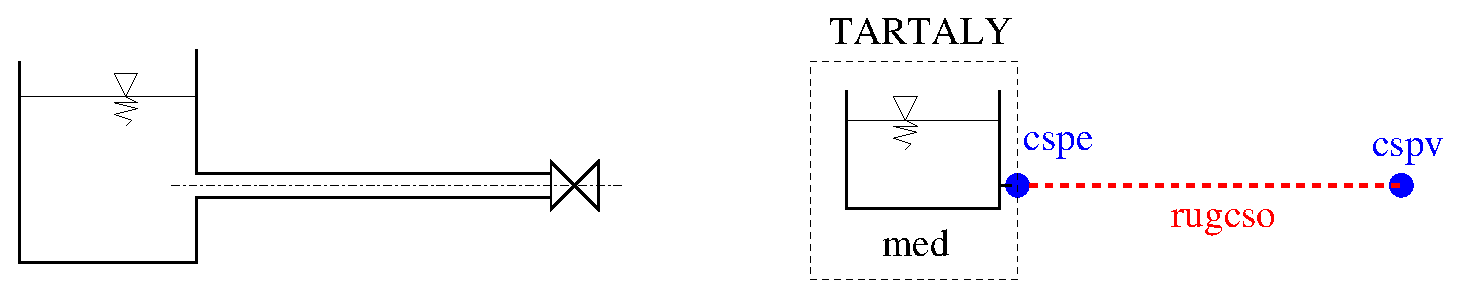
\includegraphics[width=14cm]{abrak/feladat1abra.eps}
    \caption{\label{1abra}1. feladat v�zlata}
  \end{center}
\end{figure}

\emph{Megold�s}

A cs�ben a hull�msebess�g: $E_r=\left(\frac{1}{E_f}+\frac{D}{\delta\cdot E_{cs,azb.cem.}}\right)=1.5385\times10^9\,Pa$ $\rightarrow$ $a=\sqrt{\frac{E_r}{\rho}}=1240\,m/s$.\\
Az �raml�si sebess�g: $v=\frac{\dot m}{A\cdot\rho}=0.2264\, m/s$.\\
A kialakul� nyom�sugr�s: $\Delta p=\rho\cdot a\cdot \Delta v=2.81\,bar$.

%\begin{center}
%  \begin{tabular}{|l|p{8cm}|}
%    \emph{Parancs} & \emph{Magyar�zat}\\ \hline \hline
%    {\tt >> trsz('f1','f1',10)} & Szimul�ci� 10s-ig. \\ \hline
%    {\tt >> trsz\_rajz('f1','fe11','rugcso','ev','p')} & Nyom�slefut�s rajzol�sa a {\tt rugcso} elem elej�n �s v�g�n (ld. \aref{1mo_abra}).\\ \hline
%  \end{tabular}
%\end{center}

\begin{figure}[ht!]
  \begin{center}
    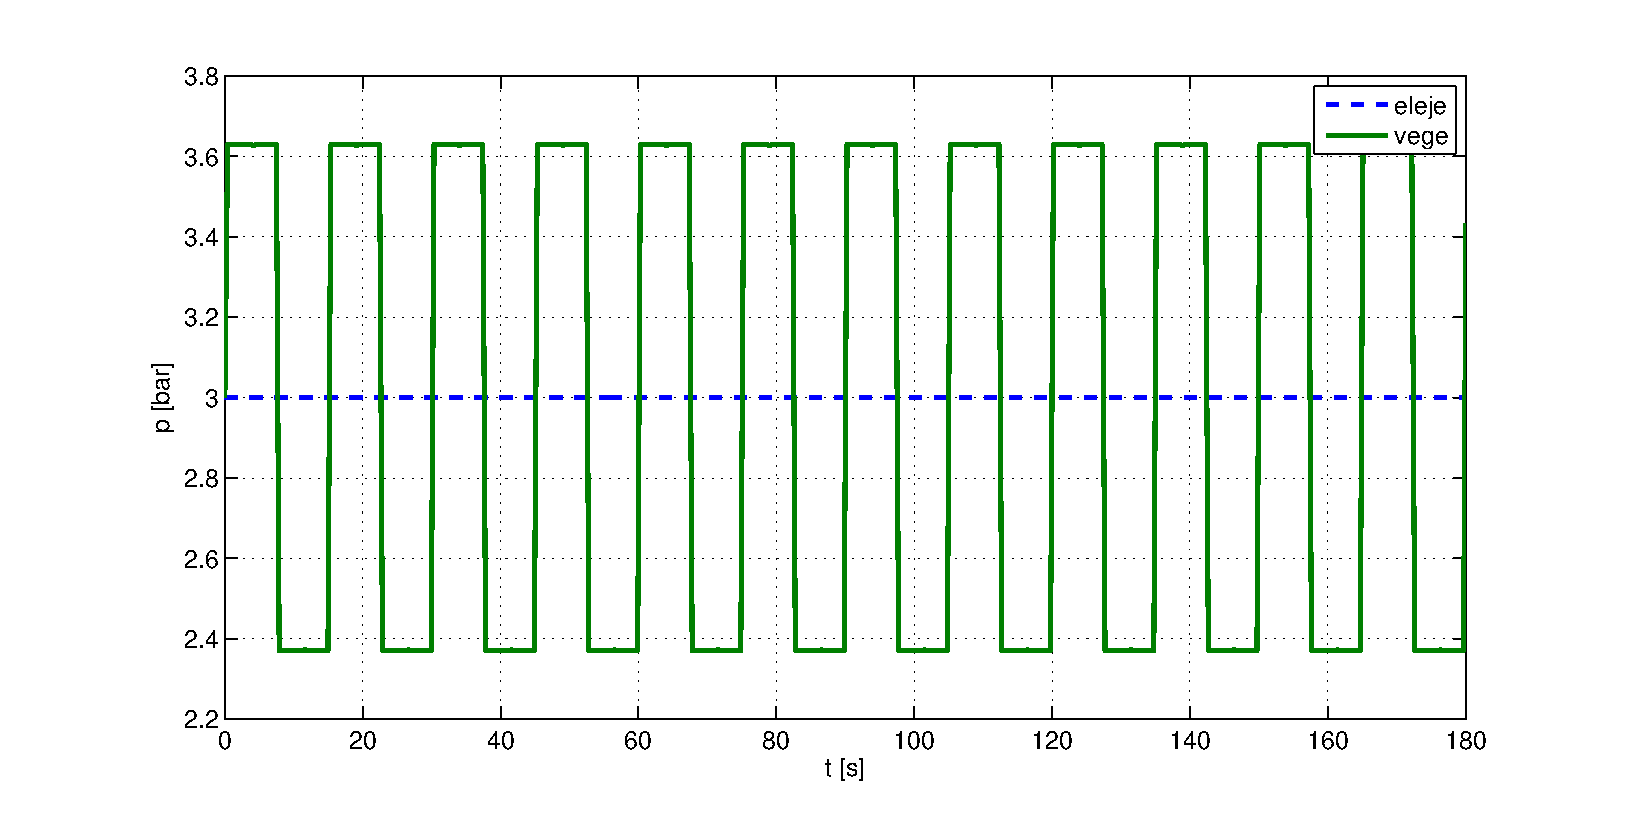
\includegraphics[width=10cm]{abrak/feladat1.eps}
    \caption{\label{1mo_abra}1. feladat megold�sa}
  \end{center}
\end{figure}

%\noindent {\bf Gyakorl� feladatok:}
%\begin{enumerate}
%\item A {\tt rugcso} bels� oszt�spontjainak sz�m�t �s geodetikus magass�g�t v�ltoztassuk meg! Mit tapasztalunk? ({\tt f1a})
%\item A {\tt rugcso} rugalmas cs�vet t�bb rugamlas cs�b�l �ll�tsuk �ssze �s ism�telj�k meg a sz�m�t�st! ({\tt f1b})
%\item A {\tt rugcso} elem a fenti esetben s�rl�d�smentes. V�gezz�k el a sz�m�t�st $\lambda=0.02$-es s�rl�d�si t�nyez�vel is! Mit tapasztalunk?
%\item N�velj�k meg a z�r�s sebess�g�t $10s$-ra. Hogyan hat ez a fell�p� maxim�lis nyom�scs�csra?
%\end{enumerate}

\vfill

\pagebreak

%-------------------------------------------------------------------------

\section{2.\,feladat (V�z�t�s s�rl�d�sos cs�ben)}

Az el�z� feladat szerinti sz�m�t�sokat v�gezz�k el vesztes�ges �raml�s eset�re is. Az �tlagos cs�s�rl�d�si t�nyez� �rt�k�t $0.02$-re vett�k fel. A megold�s \aref{2mo_abra} �br�n l�that�.

\begin{figure}[ht!]
  \begin{center}
    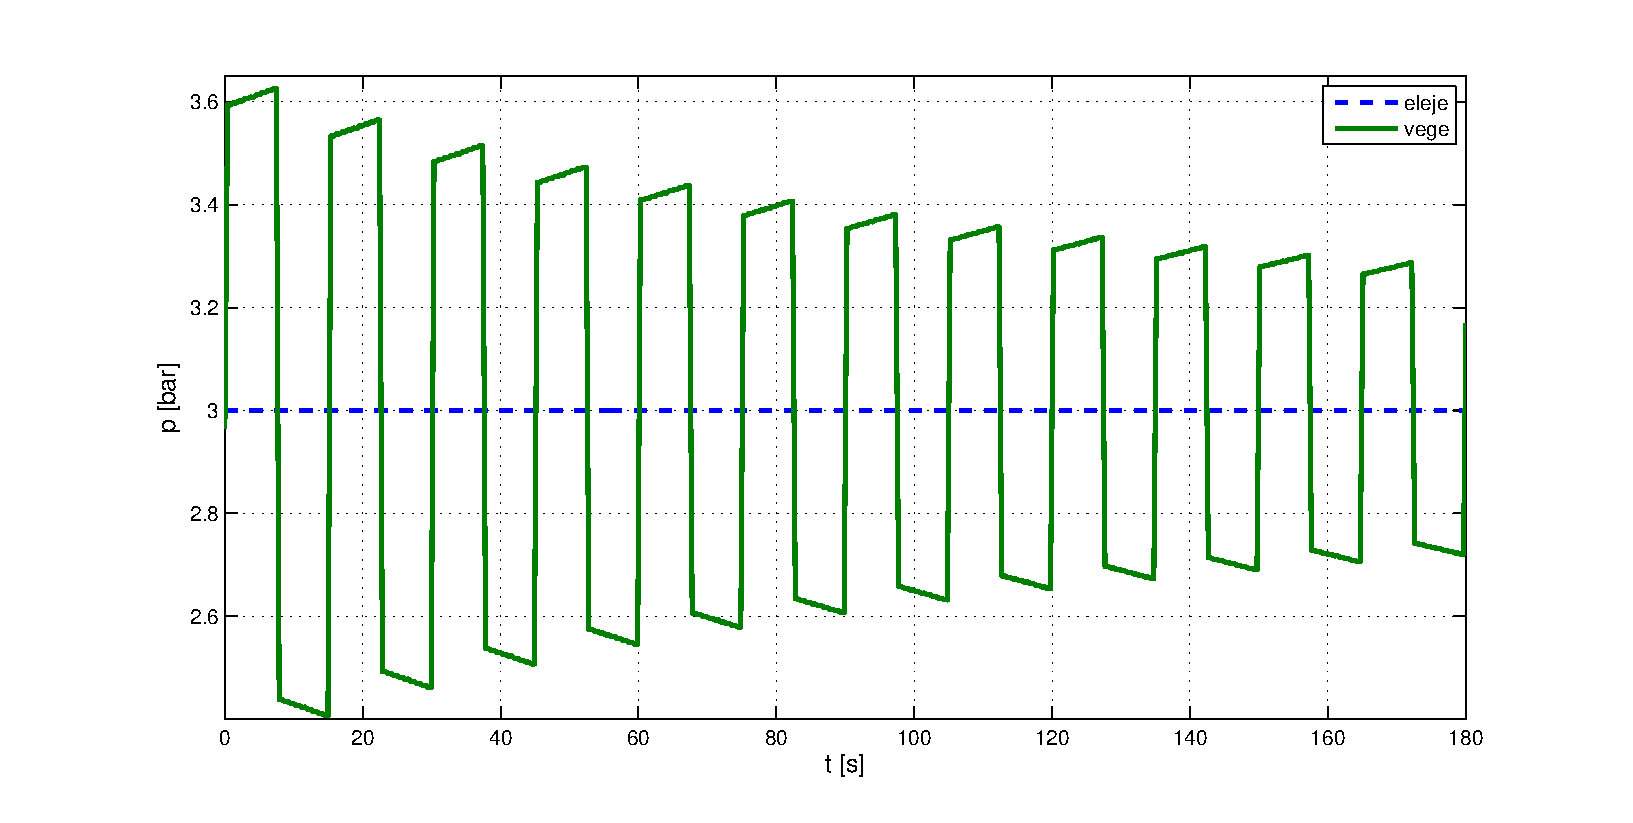
\includegraphics[width=10cm]{abrak/feladat2.eps}
    \caption{\label{2mo_abra} 2. feladat megold�sa}
  \end{center}
\end{figure}

%-------------------------------------------------------------------------

\section{3.\,feladat (Szivatty� kies�s)}

Egy szivatty�telep az als� medenc�b�l vizet sz�ll�t a fels� medenc�be. A folyad�k vissza�raml�s�t visszacsap� szelep akad�lyozza. A cs�vezet�k hossz szelv�nye \aref{3f_cso} �br�n l�that�. A cs� adatai: $L=2250\,m$, $D=0.253\,m$, $\delta=13\,mm$, $E_{cs,azb.cem.}=2.4 \times10^9\,Pa$, $E_f=2.2\times 10^9\,Pa$. 

\clearpage

\begin{figure}[ht!]
  \begin{center}
    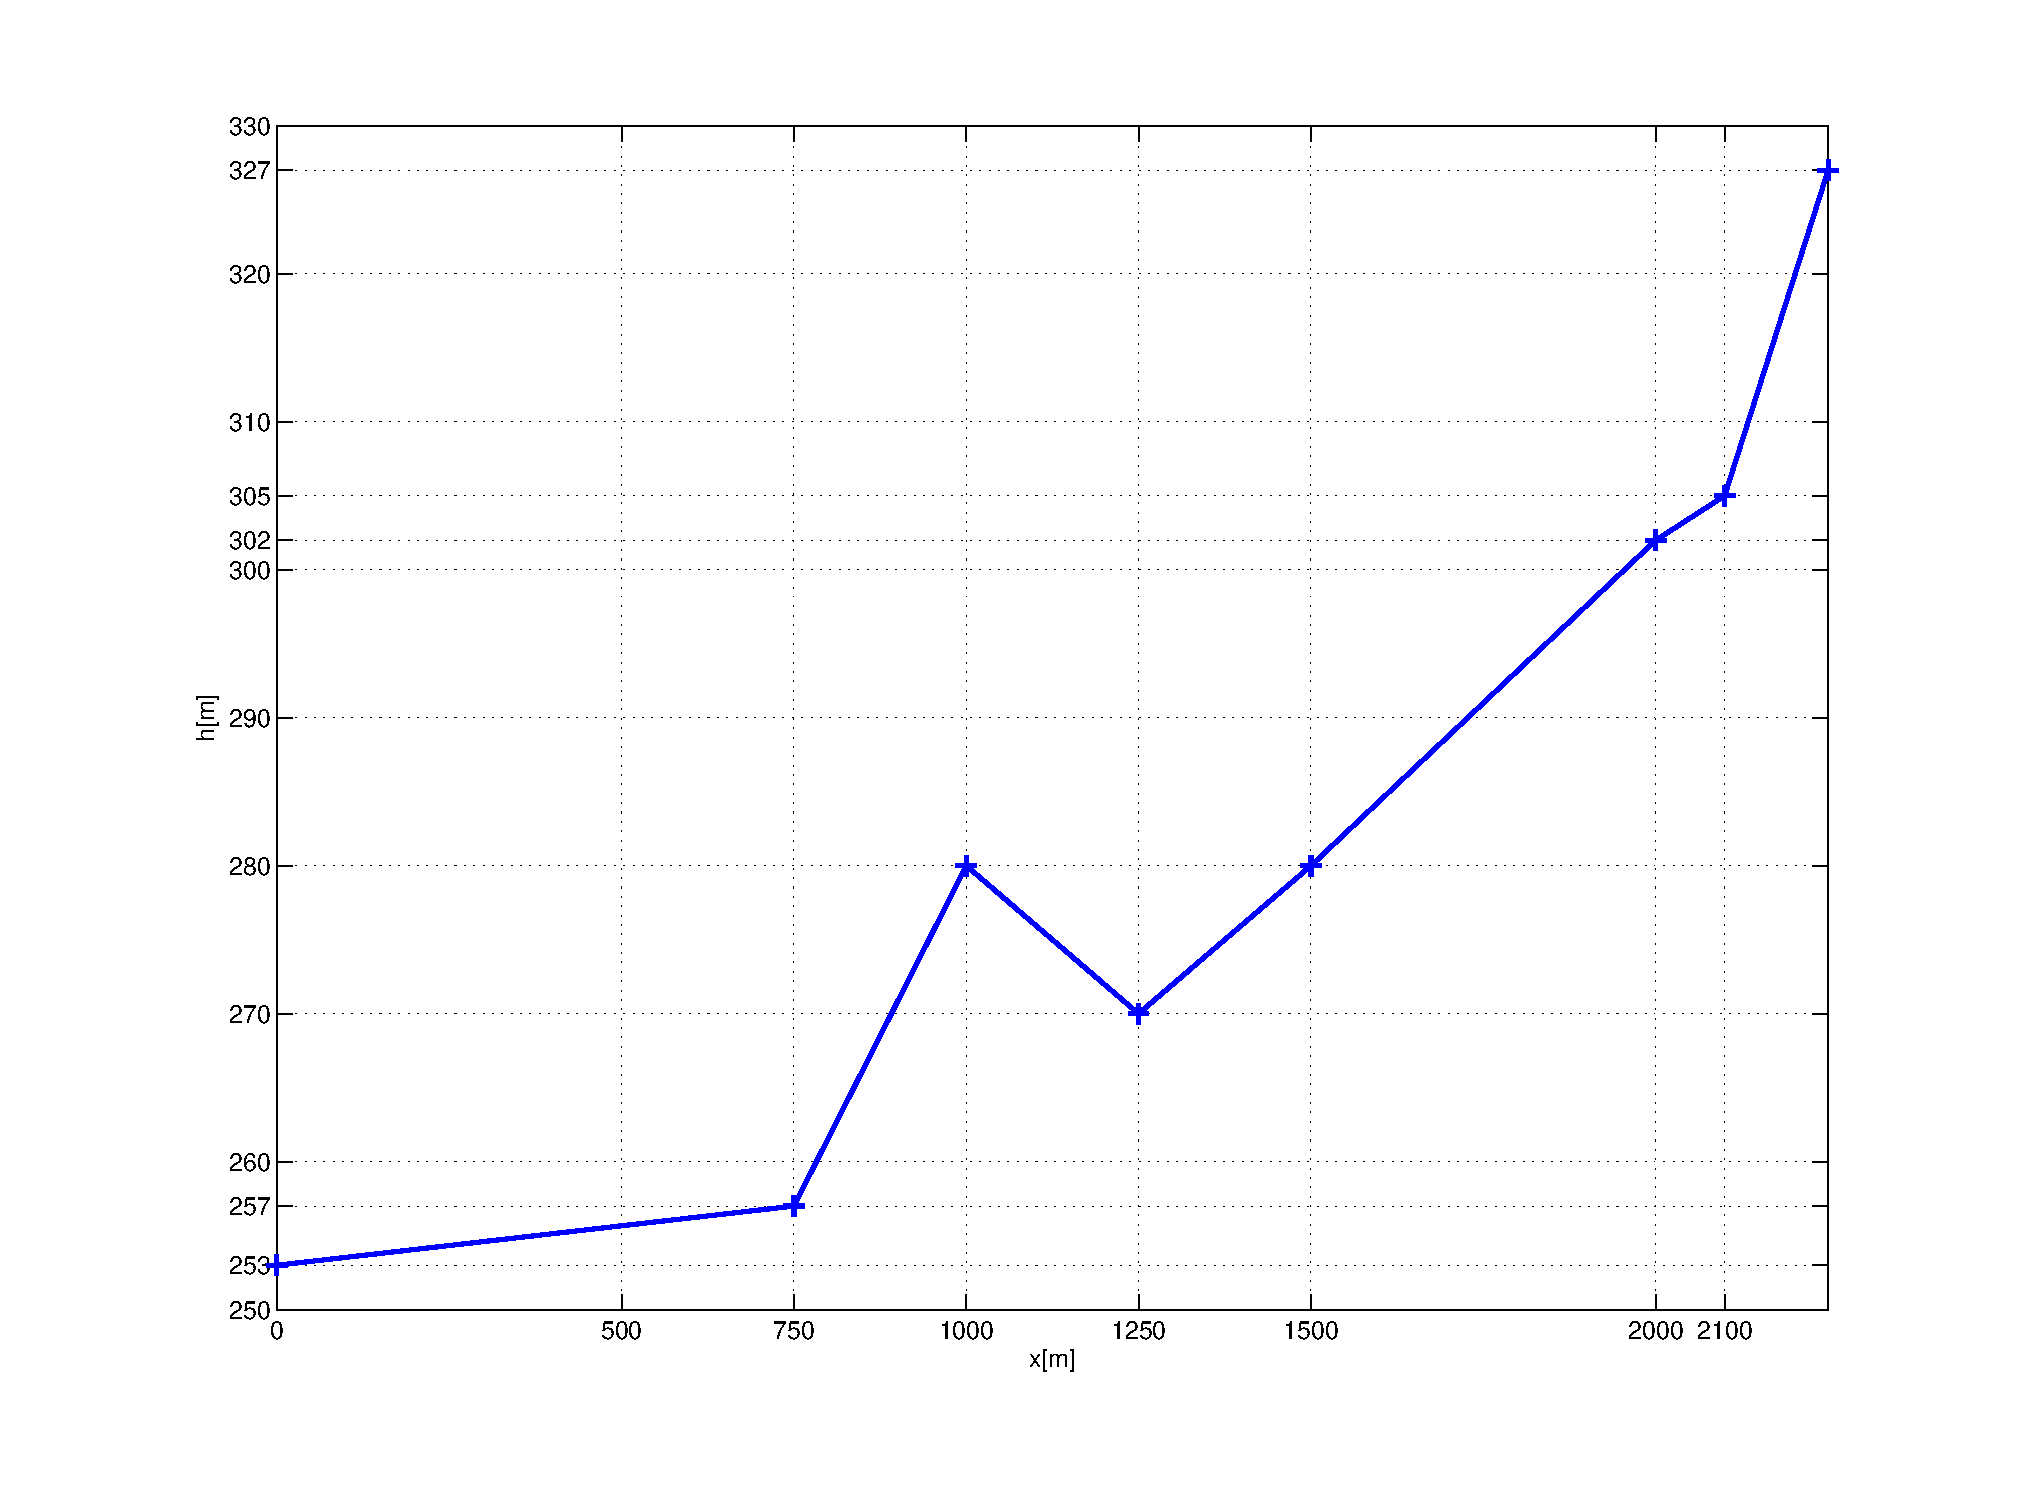
\includegraphics[width=10cm]{abrak/feladat3nyv.eps}
    \caption{\label{3f_cso} A cs� nyomvonala a 3. feladathoz.}
  \end{center}
\end{figure}

A be�p�tett b�v�rszivatty� adatai:

\begin{center}
\begin{tabular}{|c||c|c|c|}\hline
Ssz. & $Q\,[m^3/s]$ & $H\,[m]$  & $P_{be}\,[kW]$\\ \hline \hline
1    &  0.000   		& 110 & 16.8\\ \hline
2    &  0.005      & 105 & 18.0\\ \hline
3    &  0.010     	& 98  & 20.8\\ \hline
4    &  0.015      & 93  & 23.2\\ \hline
5    &  0.020     	& 88  & 25.6\\ \hline
6    &  0.025      & 84  & 28.0\\ \hline
7    &  0.030     	& 72  & 30.0\\ \hline
8    &  0.035      & 65  & 32.0\\ \hline
\end{tabular}
\end{center}

A szivatty� fordulatsz�ma $1450\ 1/perc$, a szivatty� �s motor g�pcsoport egy�ttes lend�t�nyomat�ka $GD^2=1.9\,Nm^2$. Az �tlagos cs�s�rl�d�si t�nyez� $0.029$. Sz�m�tsa ki a szivatty� �ramkimarad�sa miatt bek�vetkez� nyom�sleng�seket. Ism�telje meg a sz�m�t�st t�zszeres�re ill. sz�zszoros�ra megn�velt tehetetlens�gi nyomat�kkal! V�gezzen sz�m�t�st ac�l- ($E_{\textrm{cs,ac�l}}=2.1\times10^{11}\,Pa$) �s kem�ny polietil�n ($E_{cs,KPE}=690\times10^{6}\,Pa$) cs�vekre.

\begin{figure}[ht]
  \begin{center}
    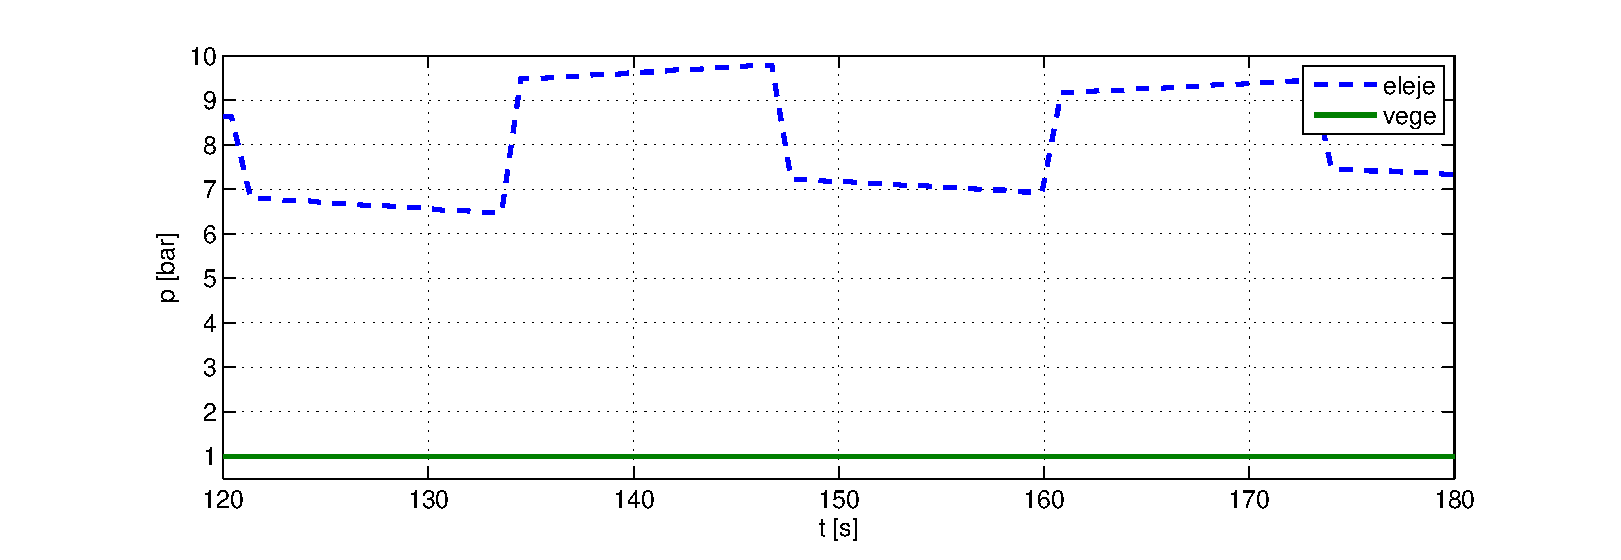
\includegraphics[width=10cm]{abrak/feladat3.eps}
    \caption{\label{3mo_abra} A 3. feladat megold�sa}
  \end{center}
\end{figure}

%-------------------------------------------------------------------------

\section{4.\,feladat (Szivatty� kies�s tol�z�rral)}

A 3.\,feladat szerinti berendez�sben a vezet�k $1500\,m$-es szelv�ny�ben egy r�szben nyitott tol�z�r van. A tol�z�r ellen�ll�s t�nyez�je $\zeta=565$. Hat�rozza meg a rendszer munkapontj�t. V�gezzen sz�m�t�st �ramkimarad�s eset�re.

(Fojt�si t�nyez�: $f=\frac{\zeta}{2A^2}$)
%
\begin{figure}[ht]
  \begin{center}
    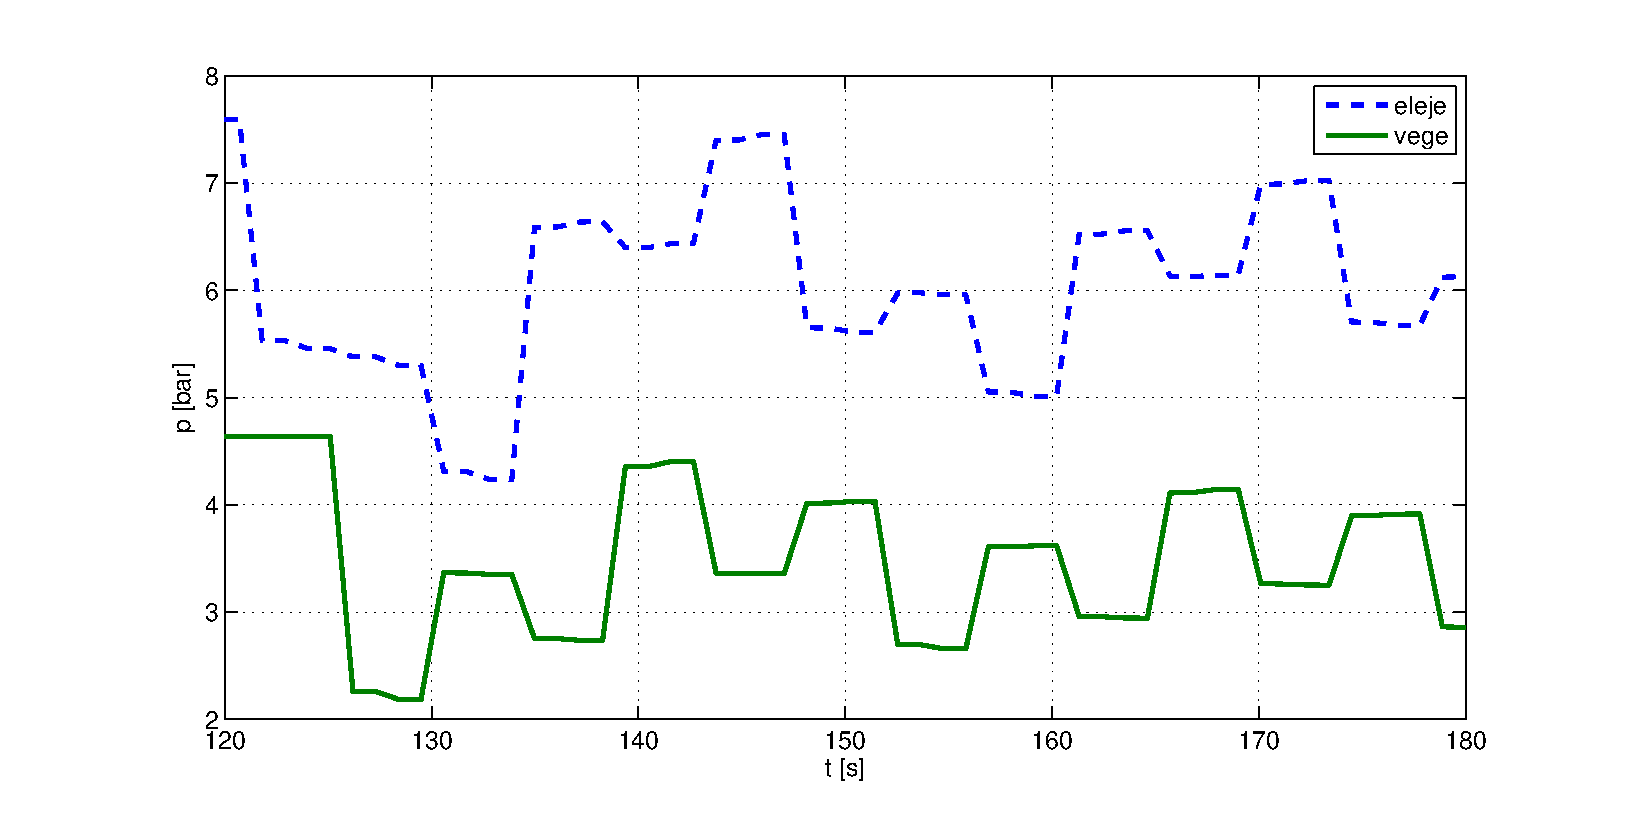
\includegraphics[width=10cm]{abrak/feladat4cso1.eps}
    \caption{\label{4mo_abra1} A 4. feladat megold�sa. $cso1$ Nyom�s-grafikonja.}
  \end{center}
\end{figure}

\begin{figure}[ht]
  \begin{center}
    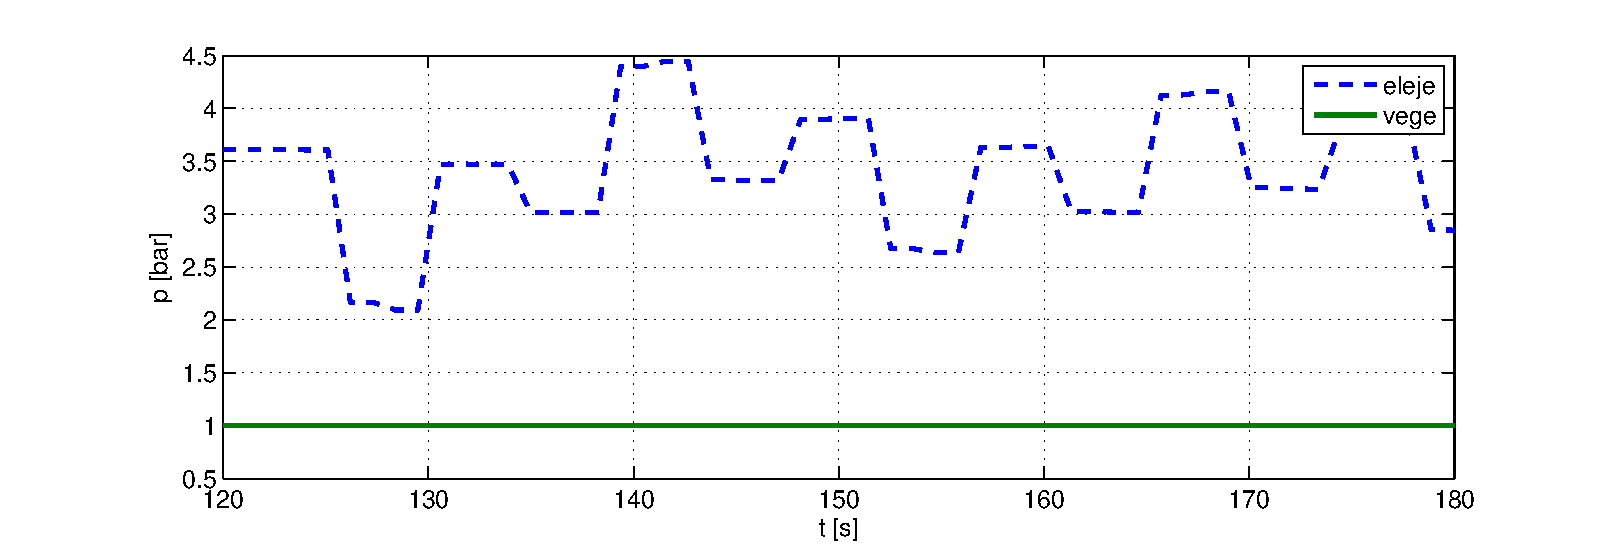
\includegraphics[width=10cm]{abrak/feladat4cso2.eps}
    \caption{\label{4mo_abra2} A 4. feladat megold�sa. $cso2$ Nyom�s-grafikonja.}
  \end{center}
\end{figure}

%-------------------------------------------------------------------------

\section{5.\,feladat (L�g�st m�retez�s)}

A 3.\,feladat szerinti berendez�sben a szivatty�kifut�s sor�n a cs�vezet�k elej�n fell�p� nyom�s meghaladja a cs�re vonatkoz� n�vleges nyom�s �rt�k�t. Hat�rozza meg sz�m�t�ssal a szivatty�telepre be�p�tend� l�g�st g�ztartalm�t ($V_{0}$) �gy, hogy az els� nyom�scs�cs ne haladja meg a $10\,bar$ �rt�ket, valamint a l�g�st ne �r�lj�n ki.

A rendszer elemeinek bek�t�si sorrendje:
\begin{enumerate}
	\item medence I.
	\item szivatty�
	\item visszacsap� szelep
	\item l�g�st
	\item rugalmas cs�
	\item medence II.
\end{enumerate}

\textbf{L�g�st:}\\
$n=1.4$, $p_{0}=3\times10^5\,Pa$, $A=0.8\,m^2$, $l=0.2\,m$, $H=2\,m$.
%
\begin{figure}[ht]
  \begin{center}
    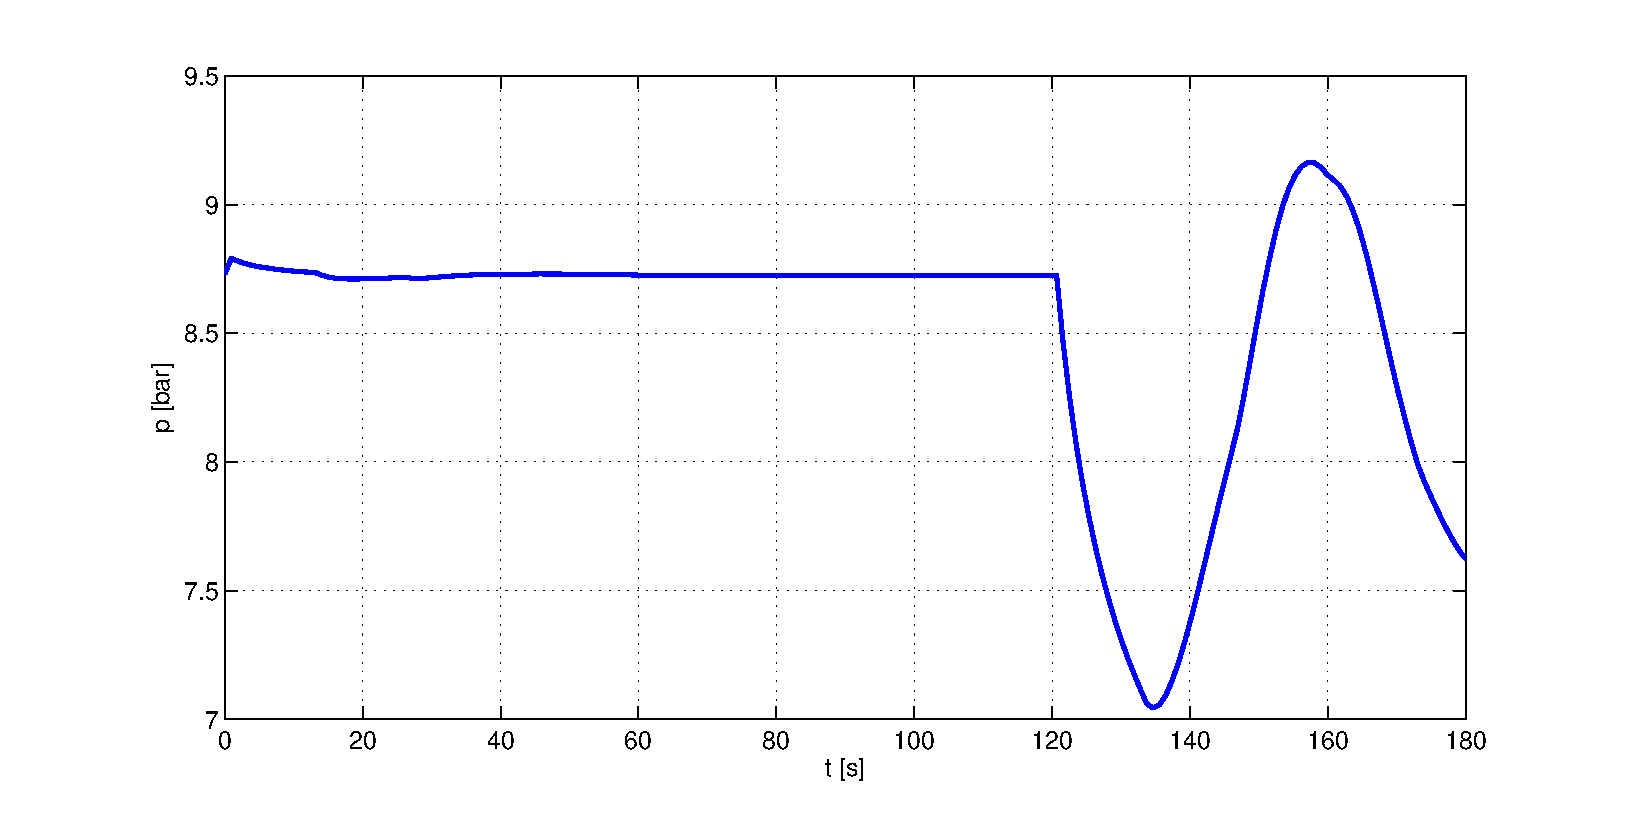
\includegraphics[width=10cm]{abrak/feladat5.eps}
    \caption{\label{7mo_abra} Az 5. feladat megold�sa.}
  \end{center}
\end{figure}
%-------------------------------------------------------------------------

\section{6. feladat (K�t�st�s leng�rendszer)}

Egy �lland� keresztmetszet� cs� k�t v�g�n egy-egy l�g�st helyezkedik el. A bal oldali l�g�st�t ,,1'', a jobb oldalit ,,2'' jel�li, a cs� param�tereit pedig ,,cs'' indexszel jel�lj�k. A l�g�st�kben a folyad�k felsz�nen a nyom�s $p_1$ ill. $p_2$. A cs� k�t v�g�n $p_{cs,1}+\frac{\rho}{2v^2}=p_1+\rho\,g\,L_1$ �s $p_{cs,2}+\frac{\rho}{2v^2}=p_2+\rho\,g\,L_2$. Az instacioner Bernoulli egyenletet alkalmazva kapjuk, hogy
%
\begin{equation*}
p_1 + \rho\,g\,L_1 = p_2 + \rho\,g\,L_2 +\lambda \frac{L_{cs}}{D}\,\frac{\rho}{2 A_{cs}^2}\,Q^2 + \frac{\rho L}{A_{cs}}\,\frac{dQ}{dt}.
\end{equation*}
%
Mivel a l�g�stben politropikus az �llapotv�ltoz�s, tudjuk, hogy $p\,V^n=konst$, �gy
%
\begin{equation*}
0=\frac{d \left(p\,V^n \right)}{dt} = \frac{dp}{dt}\,V^n + n\,V^{n-1}\,p\,\frac{dV}{dt} \quad \rightarrow \quad \frac{dp}{dt} = -n\,\frac{p}{V}\,\frac{dV}{dt}.
\end{equation*}
%
B�r $dV/dt=Q$, az el�jelekre oda kell figyelni, mert ha a cs�ben a balr�l jobbra ir�nyt tekintj�k pozit�v �raml�si ir�nynak, $dV_1/dt=-Q$ �s $dV_2/dt=Q$. Ha a l�g�st�k teljes magass�g�t $H$-val, fel�let�t $A$-val jel�lj�k, a folyad�koszlopok magass�ga
%
\begin{eqnarray*}
L_1(t) &= H_1 - \frac{V_1(t)}{A_1} = H_1 - \frac{V_{10}-\int\!Q dt}{A_1},\\
L_2(t) &= H_2 - \frac{V_2(t)}{A_2} = H_2 - \frac{V_{20}+\int\!Q dt}{A_2}.
\end{eqnarray*}
%
Teh�t a megoldand� egyenletrendszer:
%
\begin{equation*}
\left\{ 
\begin{array}{lll}
\dot Q   & = & \frac{A_{cs}}{\rho\,L_{cs}} \left( p_1-p_2+\rho\,g \left(L_1-L_2\right) - \lambda\, \frac{L_{cs}}{D}\, \frac{\rho}{2 A_{cs}^2}\,Q\,|Q|\right)\\
\dot p_1 & = &  n\,\frac{p_1}{V_{10}+z}\,Q\\
\dot p_2 & = & -\,n\,\frac{p_2}{V_{20}-z}\,Q\\
\dot z   & = & Q\\
\end{array}
\right.
\end{equation*}
%
�s $L_1=H_1 - (V_{10}+z)/A_1$, $L_2=H_2 - (V_{20}-z)/A_2$. 

Az 1. (bal oldali) l�g�st adatai: $n=1.4$, $V_0=1\,m^3$, $A=1\,m^2$, $l=0\,m$ �s $H=2\,m$. A 2. (jobb oldali) l�g�st adatai ugyanezek, kiv. $p_0=1\,bar$. A rugalmas cs� adatai: $D=0.3\,m$, $L=10\,m$, $\lambda=0$, $E_f=2.1\times 10^9\,Pa$, $E_c=2.1\times 10^{11}\,Pa$, $p_0=0$ �s ${\dot m}_0=0$. \Aref{7a_mo_abra}. �br�n a 2. l�g�st talppontj�nak a nyom�slefut�s�t vetj�k �ssze a fenti KDER numerikus (Runge-Kutta) megold�s�val.

\begin{figure}[ht]
  \begin{center}
    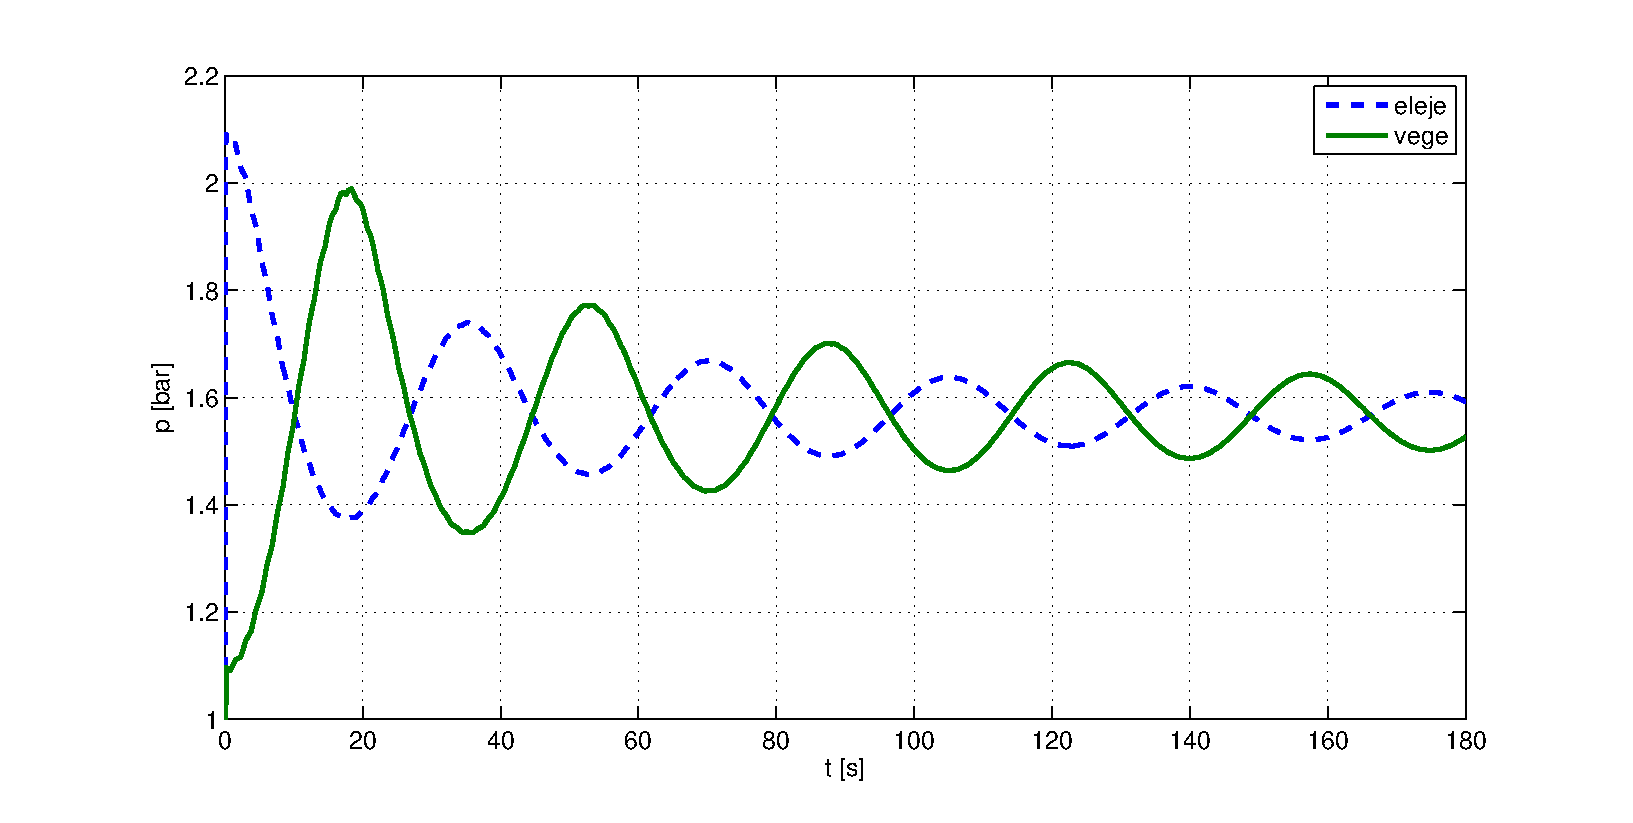
\includegraphics[width=10cm]{abrak/feladat6.eps}
    \caption{\label{7a_mo_abra} A 6. feladat megold�sa.}
  \end{center}
\end{figure}

%-----------------------

\section{7.\,feladat (Ny�ltfelsz�n� �raml�s)}
K�t akn�b�l �s egy az azokat �sszek�t� k�r keresztmetszet� csatorn�b�l �ll� h�l�zat adatai a k�vetkez�k: $A_{1}=10.5\,m^2$,\\ $h_{1,min}=98.43\,m$, $h_{1,max}=105\,m$, $h_{1,0}=1.5\,m$.\\
$A_{2}=10.5\,m^2$, $h_{2,min}=101.6\,m$, $h_{2,max}=106.07\,m$,\\ $h_{2,0}=0.3\,m$.
A kettes sz�m� akn�ba $(-)50\,m^{3}/h$ bet�pl�l�st vegyen figyelembe!

$D=0.4\,m$, $L=941\,m$, $z_e=102\,m$, $z_v=101\,m$, $n=0.013$, $y_0=0.01\,m$.

Haszn�lja az \texttt{option,dt\_save,1.0} parancsot a .tpr f�jl els� sor�ban az 1 m�sodpercenk�nt t�rt�n� adatment�shez. (A kimenetei f�jlban l�that�an nem pontosan a megadott id�k�z�nk�nt t�rt�nik a mintav�tel, ez a vizsg�lt szakasz hossz�t�l --feloszt�s�nak finoms�g�t�l-- f�gg.)

�br�zolja a csatorna $Q-t$ diagramj�t, valamint az ,,1.'' sz�m� akna v�zszint v�ltoz�s�t az id� f�ggv�ny�ben.

\begin{figure}[ht]
  \begin{center}
    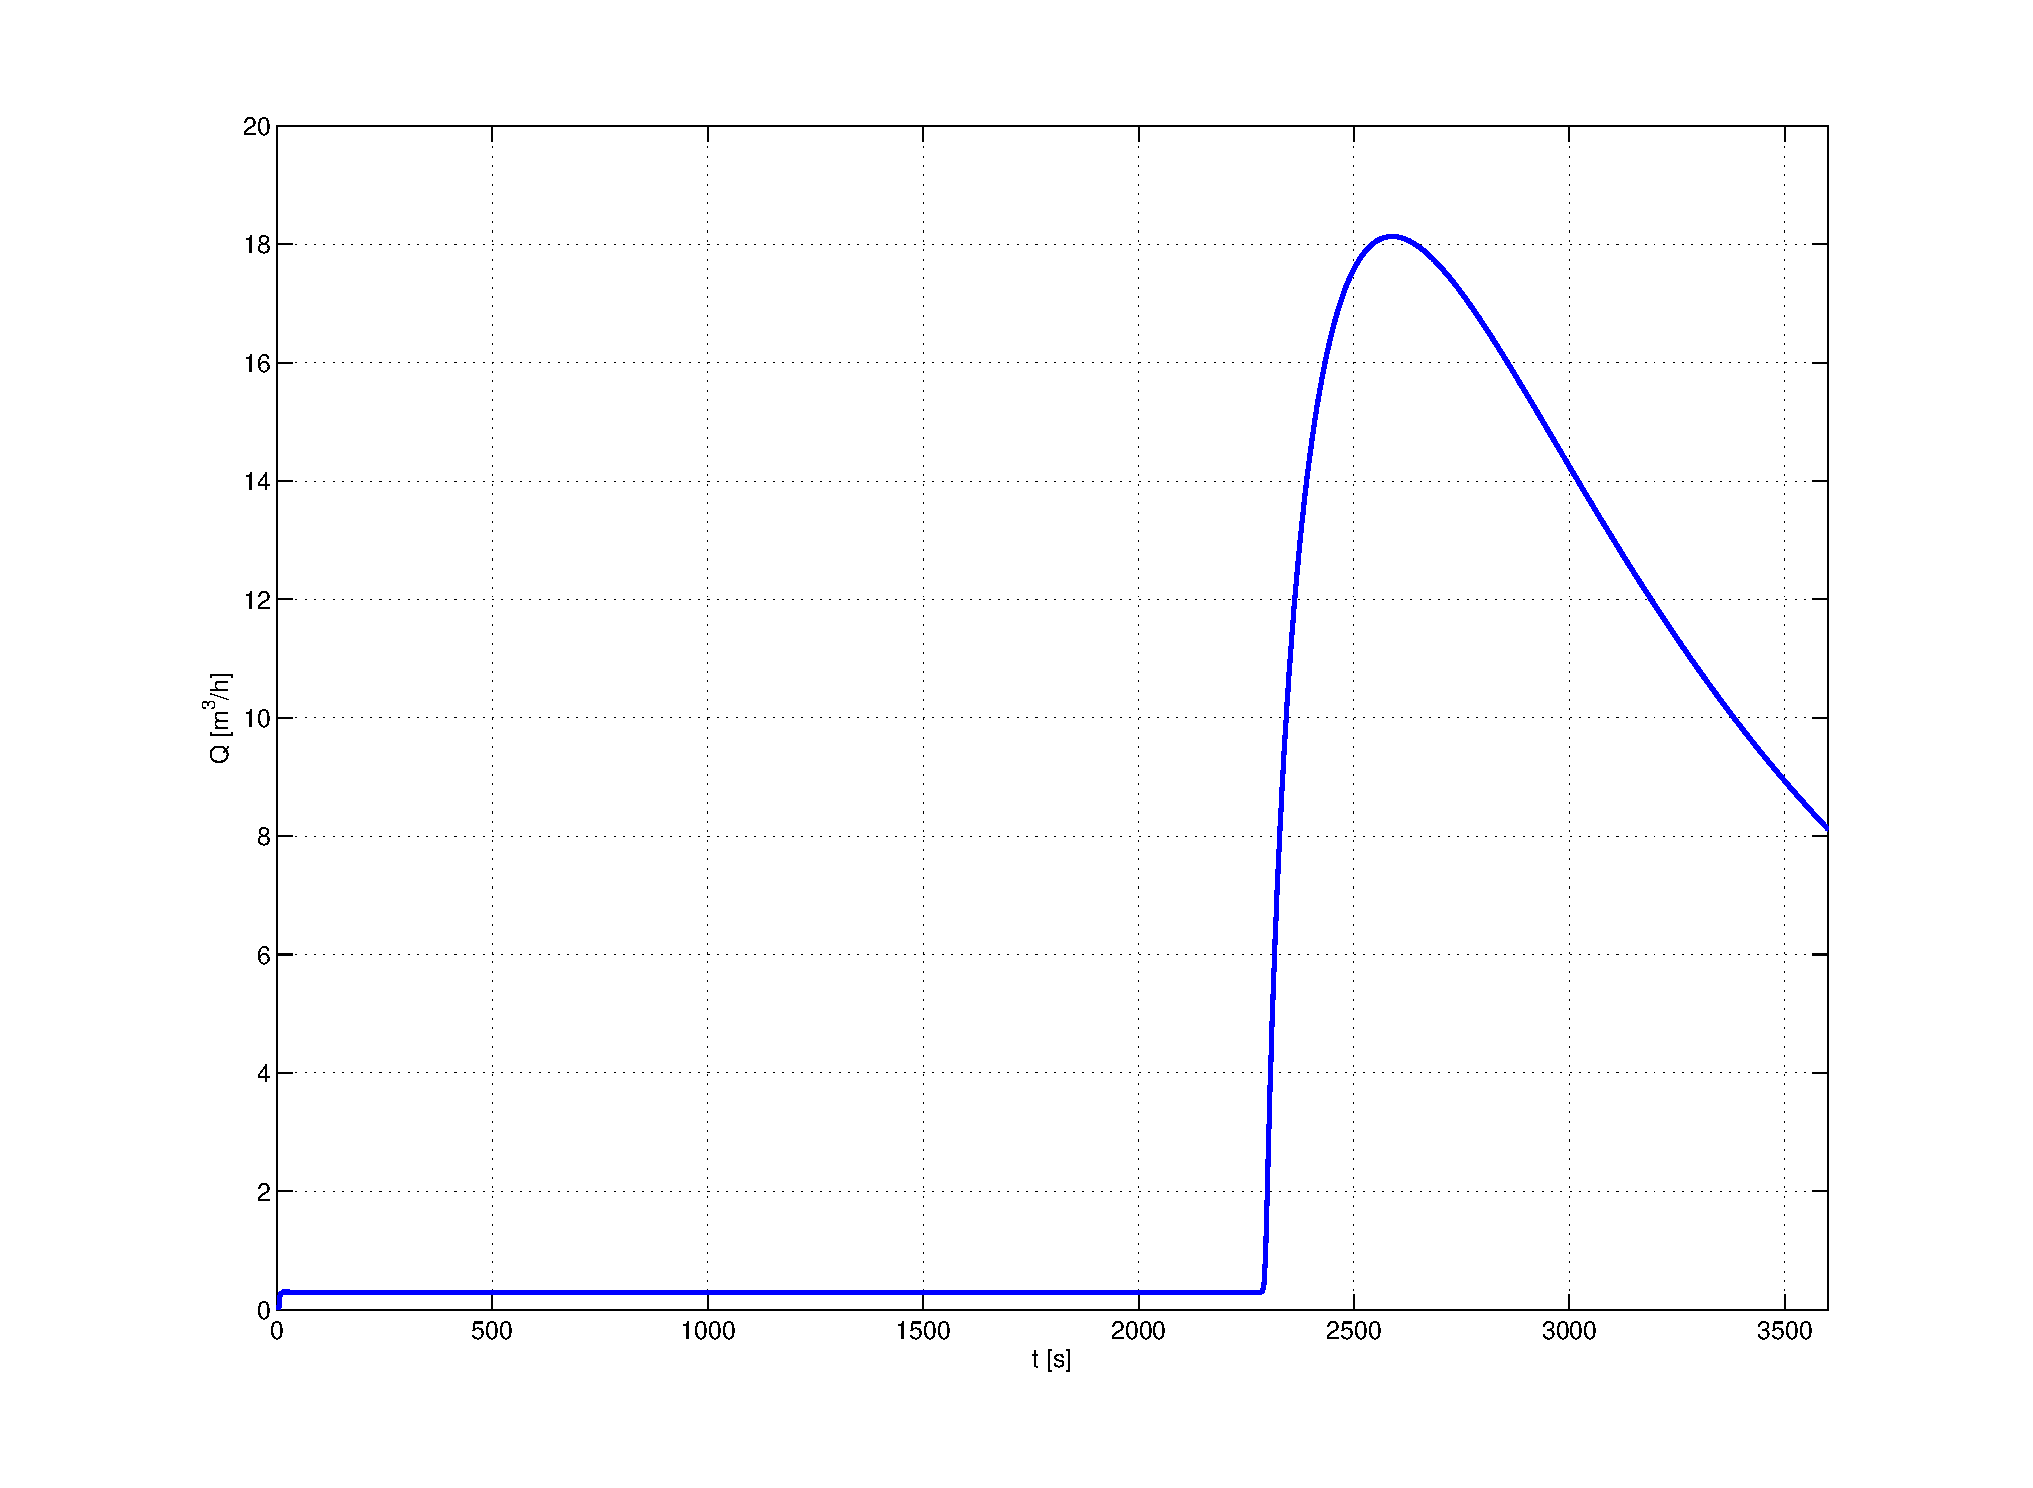
\includegraphics[width=10cm]{abrak/feladat7qt.eps}
    \caption{\label{7mo_abra1} A 7. feladat megold�sa. $Q-t$ diagram.}
  \end{center}
\end{figure}

\begin{figure}[ht]
  \begin{center}
    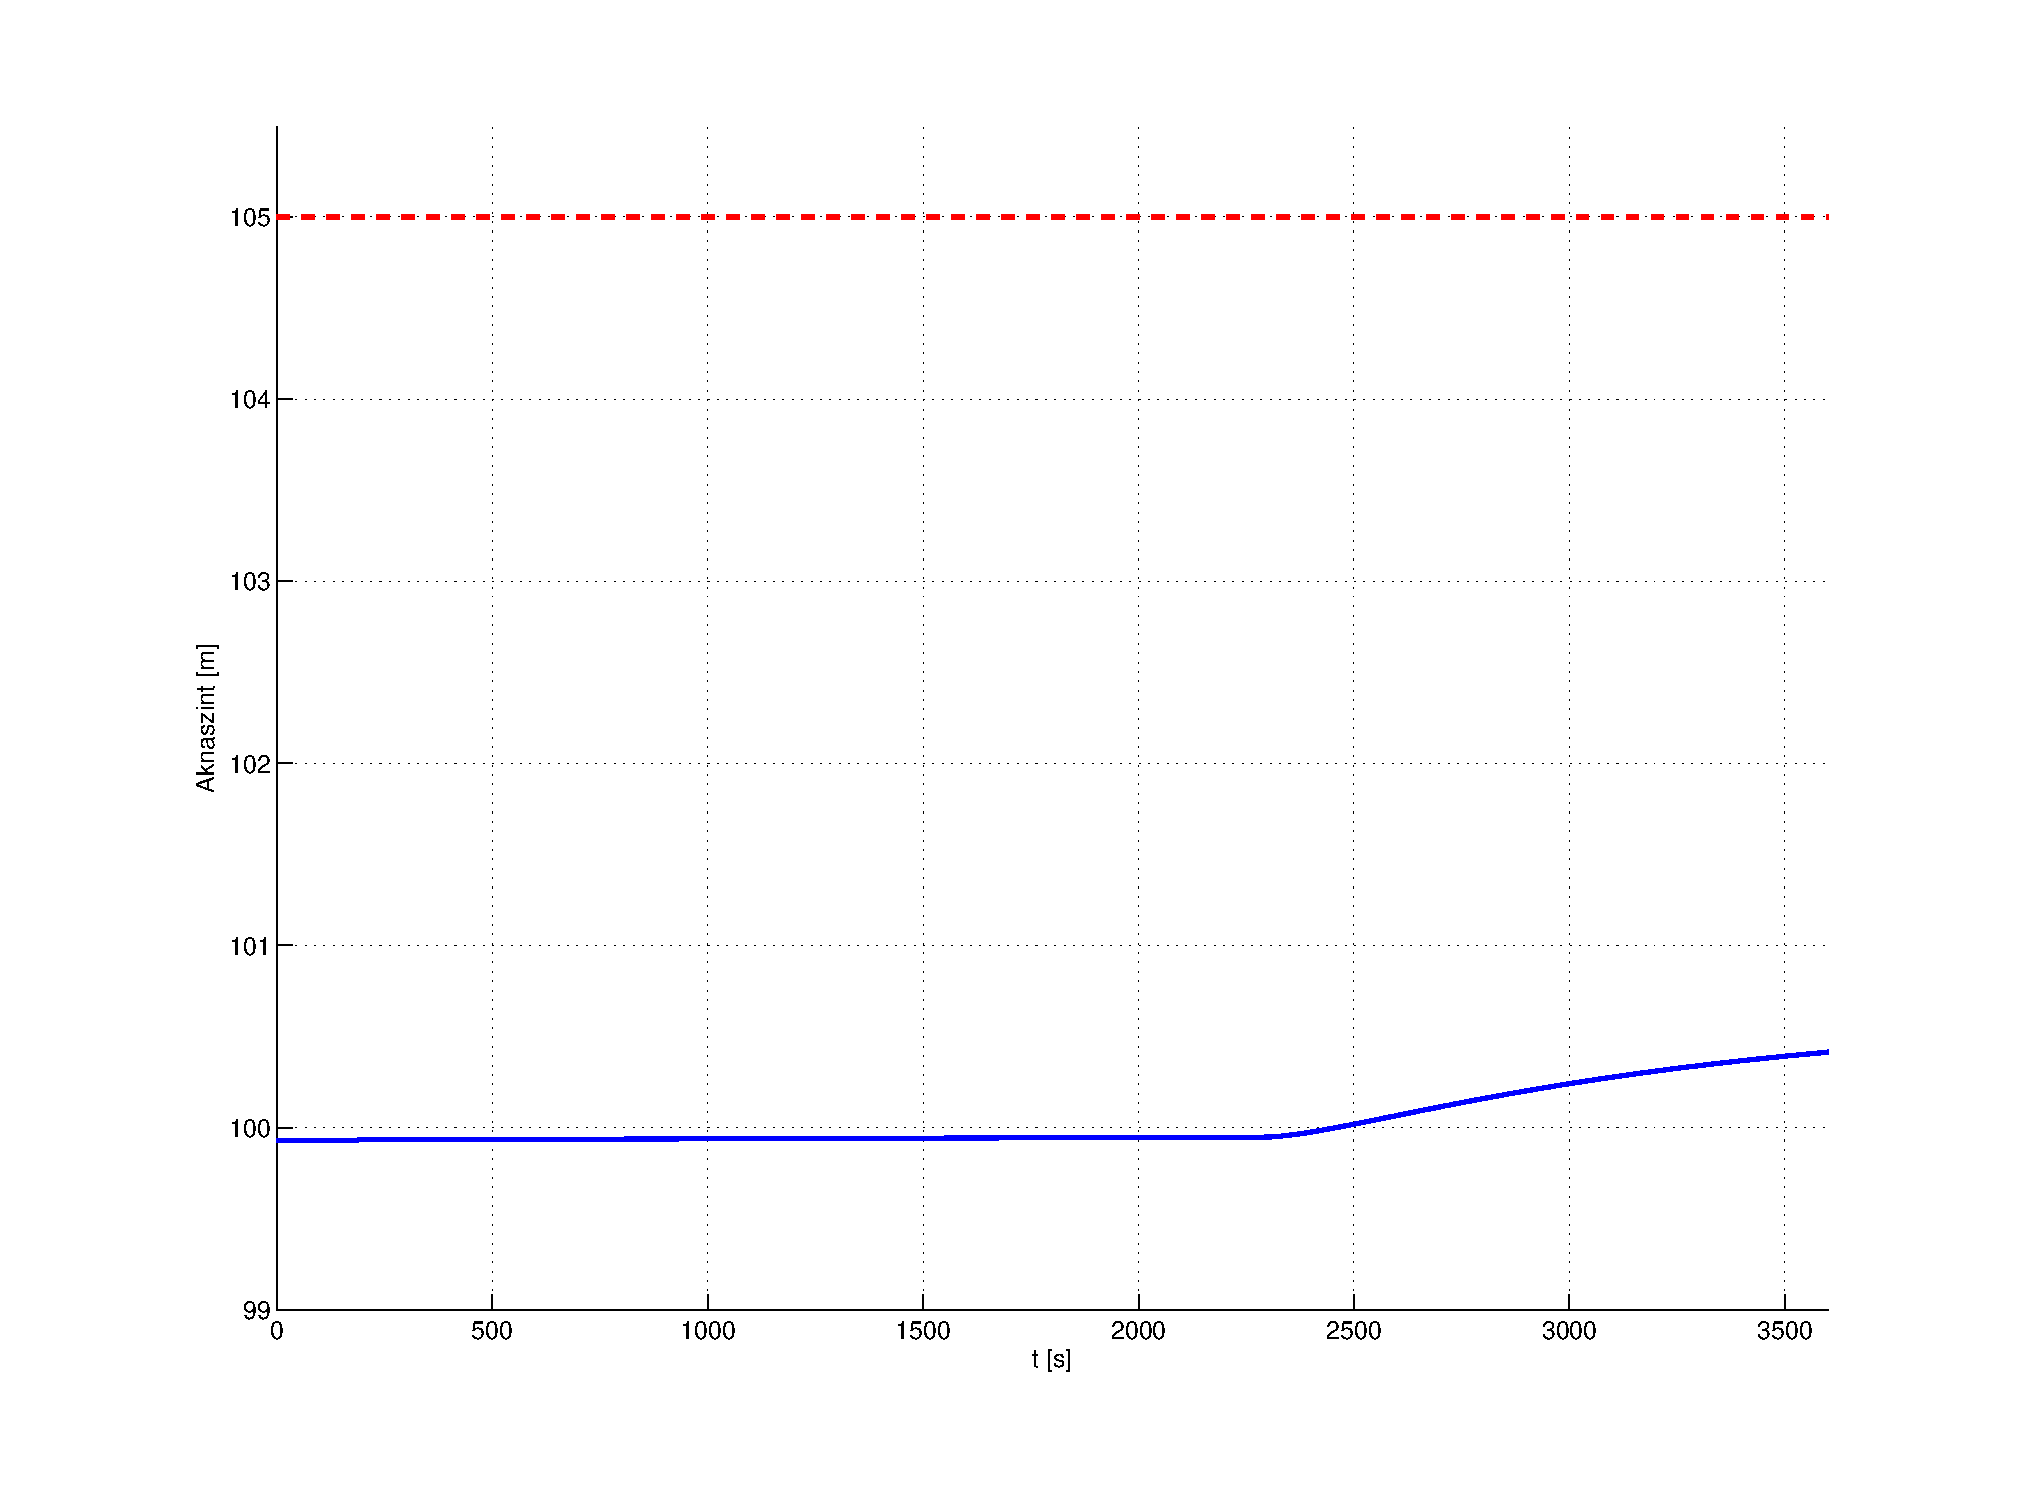
\includegraphics[width=10cm]{abrak/feladat7yt.eps}
    \caption{\label{7mo_abra2} A 7. feladat megold�sa. $y-t$ diagram.}
  \end{center}
\end{figure}
\vfill
\clearpage
%-------------------------------

\section{8.\,feladat (�temel�szivatty�s csatornarendszer)}
Adott az al�bbi kapcsol�si v�zlaton l�that� csatornah�l�zat. Az $ak01$ jel� akn�b�l a $cs1000$ k�r keresztmetszet� csatorn�n kereszt�l jut el a szennyv�z
az $at01$ jel� �temel� akn�ba. K�t szivatty� ($szat01$ �s $szat01s$) az �temel�b�l egy $ny1$ jel� nyom�vezet�ken kereszt�l sz�ll�tja 
a szennyvizet az $szt$ akn�ba. Ez ut�bbi akna a szennyv�ztiszt�t� telepet hivatott modellezni, ez�rt nagy keresztmetszettel rendelkezik.
Az �temel� akn�k modellez�s�hez a kor�bban m�r haszn�lt akna t�pus� elemet egy vagy t�bb szivatty�val k�tj�k �ssze.
Ezek egy �gynevezett nyom�vezet�ken kereszt�l sz�ll�tj�k el a szennyvizet az �temel�b�l. A szivatty�k m�k�d�s�t szintkapcsol�k
vez�rlik, melyek bekapcsol�si v�zmagass�gaik elt�r�ek. Amennyiben teh�t a f�szivatty� nem k�pes elegend� szennyvizet sz�ll�tani --$at01$-be �rkez� t�l nagy t�rfogat�ram miatt-- a seg�dszivatty� is m�k�dni kezd.

�br�zolja az $at01$ akna szintv�ltoz�s�t �s a szivatty�k fordulatsz�m�t az id� f�ggv�ny�ben azt al�bbi adatok alapj�n:

\textbf{Akna:}\\
$A_{szt}=5000\,m^2$, $h_{szt,min}=108\,m$, $h_{szt,max}=116\,m$, $h_{szt,0}=0.2\,m$\\
$A_{at01}=1.5\,m^2$, $h_{at01,min}=98.43\,m$, $h_{at01,max}=105.22\,m$, $h_{at01,0}=1.5\,m$\\
$A_{ak02}=28.3\,m^2$, $h_{ak02,min}=104.6\,m$, $h_{ak02,max}=106.07\,m$, $h_{ak02,0}=0.4\,m$

\textbf{Csatorna:}\\
$D_{cs}=0.4\,m$, $L_{cs}=941\,m$, $z_{cs,e}=104.81\,m$, $z_{cs,v}=101.11\,m$, $n=0.013$, $y_{cs,0}=0.05\,m$

\textbf{Nyom�vezet�k:}\\
$D_{ny}=0.3\,m$, $L_{ny}=1402\,m$, $\lambda=0.015$, $z_{ny,e}=98.6\,m$, $z_{ny,v}=110.52\,m$.

\textbf{Szivatty�:}\\
$D_{szat01,s}=0.3\,m$, $D_{szat01,n}=0.3\,m$, tranziens\ =\ 5, $n_{szat01}=1440~ 1/perc$, $h_{szat01,ki}=100.23\,m$, $h_{szat01,be}=99.03\,m$.
\begin{center}
\begin{tabular}{|c||c|c|c|}\hline
Ssz. & $Q\,[m^3/s]$ & $H\,[m]$  & $P_{be}\,[kW]$\\ \hline \hline
1    &  0.0000     	& 44.4  & 1\\ \hline
2    &  0.0280      & 38.1  & 1\\ \hline
3    &  0.0520      & 31.3  & 1\\ \hline
4    &  0.0750      & 24.4  & 1\\ \hline
5    &  0.0870      & 20.5  & 1\\ \hline
6    &  0.1030      & 13.9  & 1\\ \hline
7    &  0.1150      & 6.9   & 1\\ \hline
\end{tabular}
\end{center}

$D_{szat01s,s}=0.3\,m$, $D_{szat01s,n}=0.3\,m$, tranziens\ =\ 5, $n_{szat01s}=1440~ 1/perc$, $h_{szat01s,ki}=100.63\,m$, $h_{szat01s,be}=99.03\,m$.
\begin{center}
\begin{tabular}{|c||c|c|c|}\hline
Ssz. & $Q\,[m^3/s]$ & $H\,[m]$  & $P_{be}\,[kW]$\\ \hline \hline
1    &  0.0000     	& 44.4  & 1\\ \hline
2    &  0.0280      & 38.1  & 1\\ \hline
3    &  0.0520      & 31.3  & 1\\ \hline
4    &  0.0750      & 24.4  & 1\\ \hline
5    &  0.0870      & 20.5  & 1\\ \hline
6    &  0.1030      & 13.9  & 1\\ \hline
7    &  0.1150      & 6.9   & 1\\ \hline
\end{tabular}  
\end{center}

A teljes�tm�ny �s fordulatsz�m �rt�kei a sz�m�t�s szempontj�b�l k�z�mb�sek, de $n,P\neq 0.$

\begin{figure}[ht]
  \begin{center}
    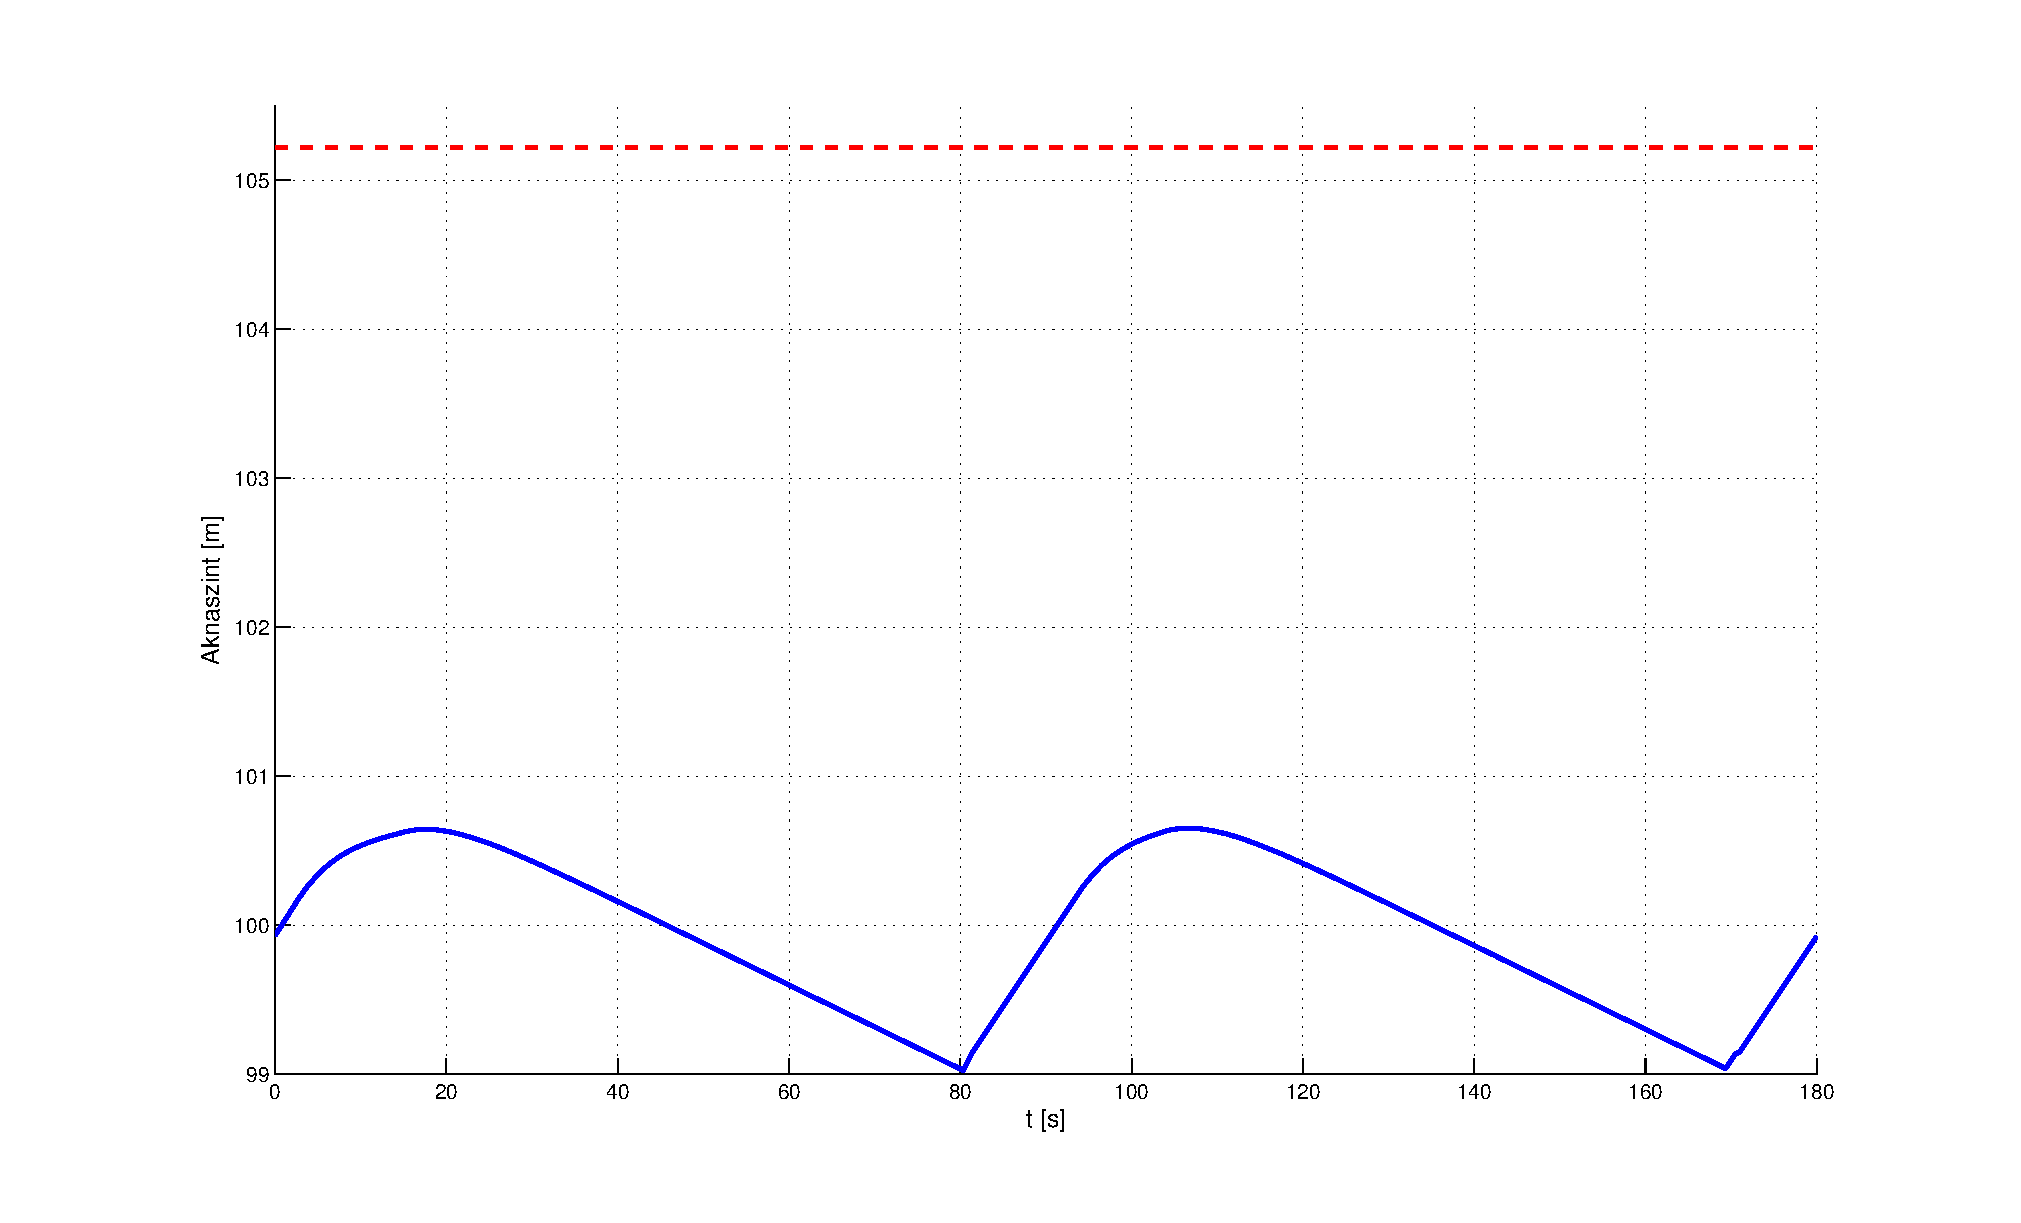
\includegraphics[width=10cm]{abrak/feladat8at01.eps}
    \caption{\label{8mo_abra1} A 8. feladat megold�sa. \textit{at01} akna v�zszintv�ltoz�sa}
  \end{center}
\end{figure}

\begin{figure}[ht]
  \begin{center}
    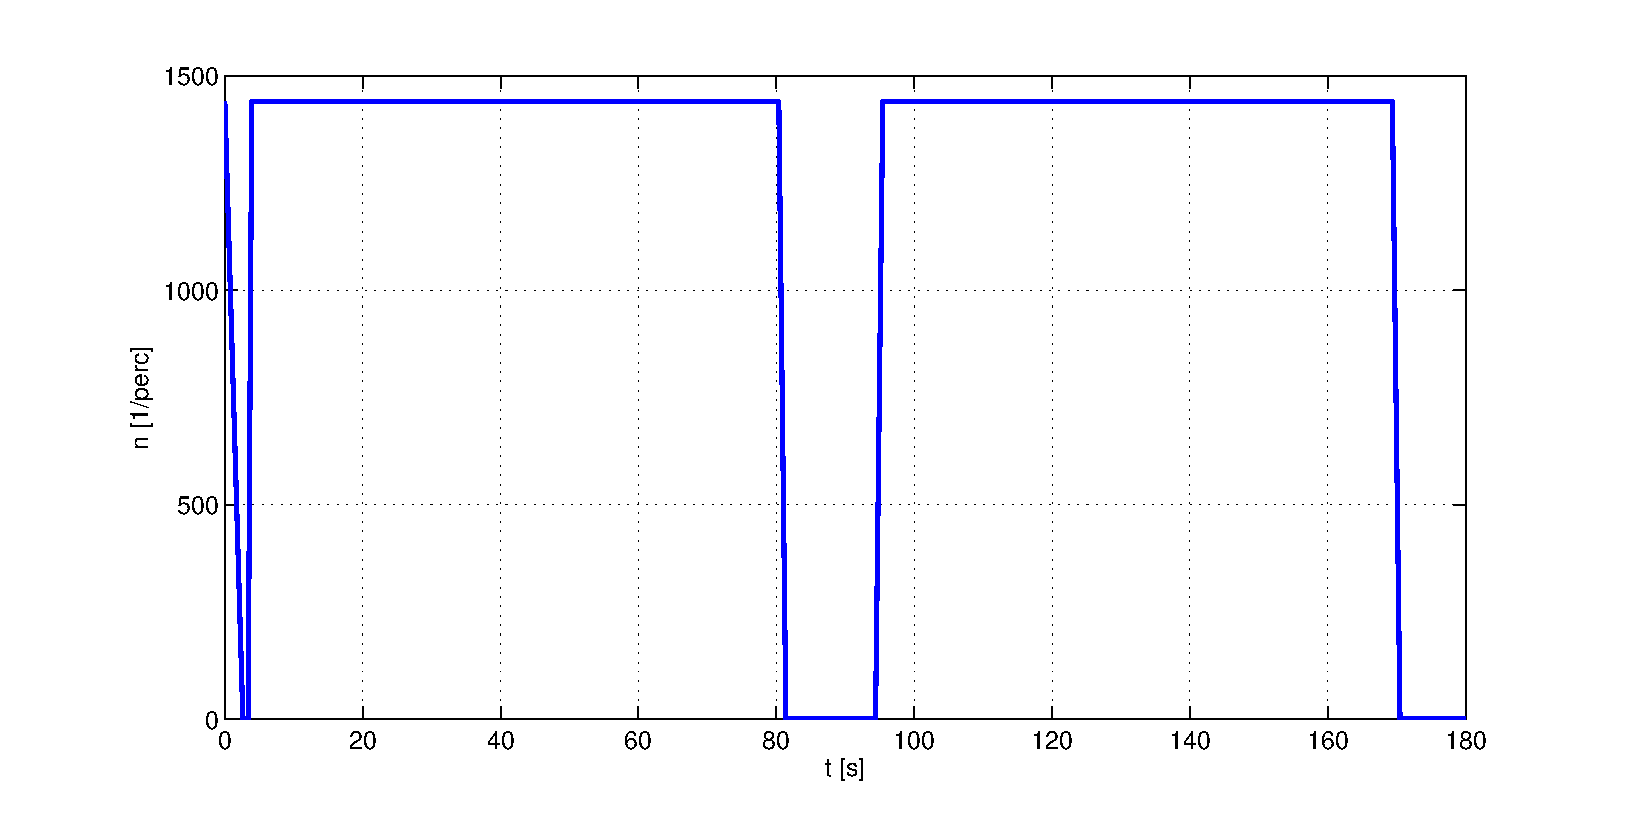
\includegraphics[width=10cm]{abrak/feladat8szat01.eps}
    \caption{\label{8mo_abra2} A 8. feladat megold�sa. \textit{szat01} szivatty� fordulatsz�ma}
  \end{center}
\end{figure}

\begin{figure}[ht!]
  \begin{center}
    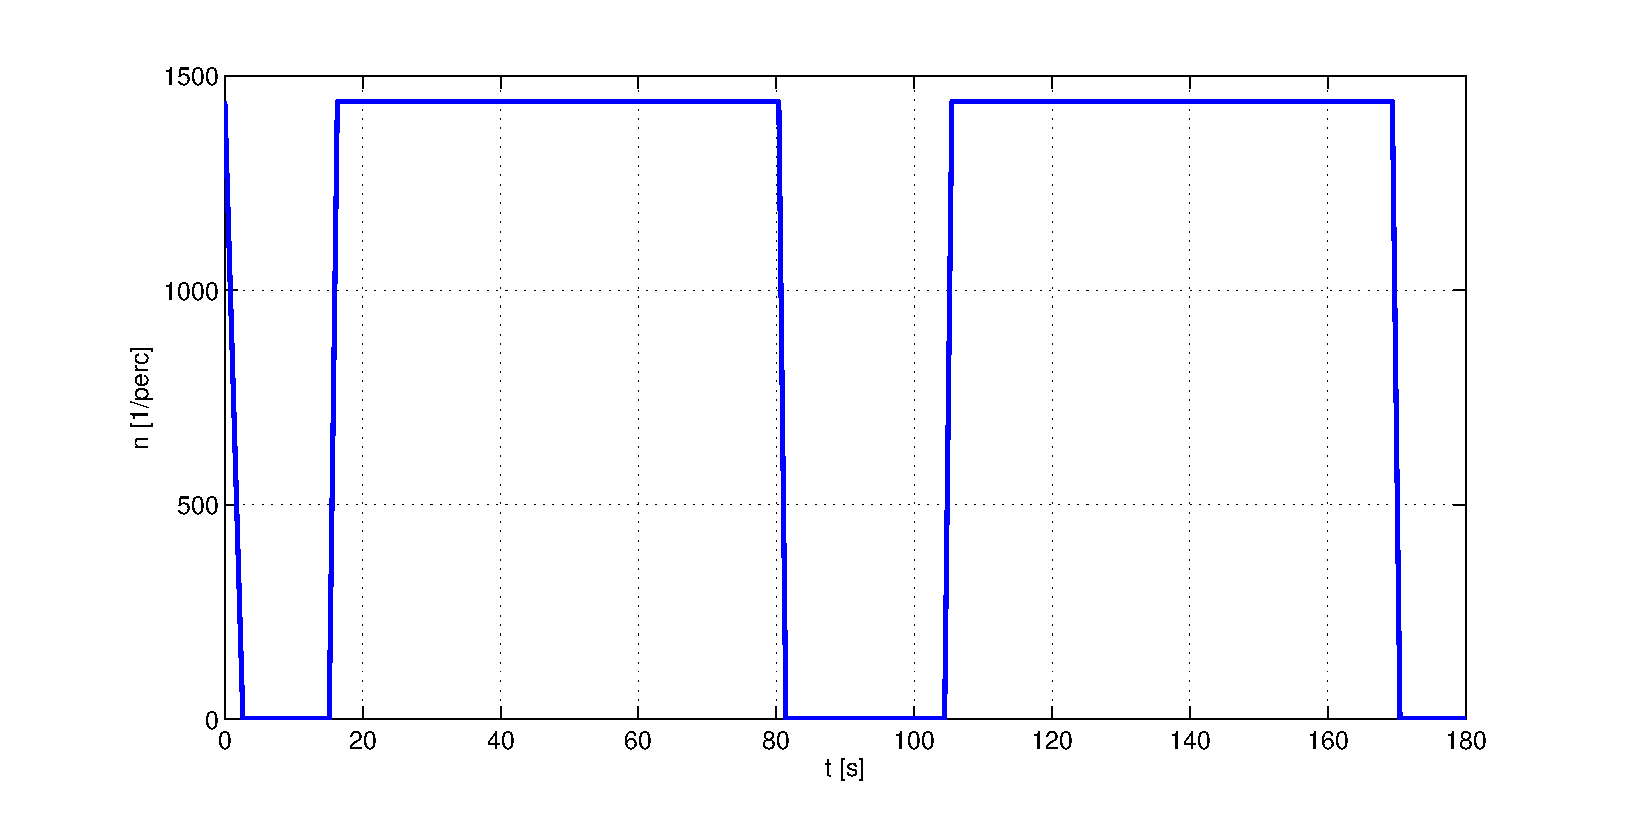
\includegraphics[width=10cm]{abrak/feladat8szat01s.eps}
    \caption{\label{8mo_abra3} A 8. feladat megold�sa. \textit{szat01} szivatty� fordulatsz�ma}
  \end{center}
\end{figure}
\vfill
\clearpage
%-----------------------------------
\section{9.\,feladat (V�r�raml�s)}
\subsection{,,A'' r�sz}
Az al�bbi modell egy v�r�raml�si modellt hivatott reprezent�lni, melynek megval�s�t�s�hoz sok, eddig nem haszn�lt �p�t�elemekkel kell dolgoznunk. A sz�v (mint v�ltoz� t�meg�ram) hivatott a $\rho=1000\,kg/m^3$ s�r�s�g� k�zeget az �rrendszer (viszkoelasztikus cs�) fel� pump�lni, a k�vetkez� t�bl�zatban foglaltak szerint.

\begin{center}
\begin{tabular}{|c||c|c|}\hline
Ssz.  & $t\,[s]$ & $Q\,[m^3/h]$\\ \hline \hline
1     &  0.00  		   & 0\\ \hline
2     &  0.01        & 5.11875E-02\\ \hline
3     &  0.02        & 0.099750\\ \hline
4     &  0.03        & 0.145688\\ \hline
5     &  0.04        & 0.189000\\ \hline
6     &  0.05        & 0.229688\\ \hline
7     &  0.06        & 0.267750\\  \hline
8     &  0.07     	 & 0.303188\\ \hline
9     &  0.08        & 0.336000\\ \hline
10    &  0.09        & 0.366188\\ \hline
11    &  0.10        & 0.393750\\ \hline
12    &  0.11        & 0.418688\\ \hline
13    &  0.12        & 0.441000\\ \hline
14    &  0.13        & 0.460688\\  \hline
15    &  0.14        & 0.477750\\ \hline
16    &  0.15        & 0.492188\\ \hline
17    &  0.16        & 0.504000\\ \hline
18    &  0.17        & 0.513188\\ \hline
19    &  0.18        & 0.519750\\ \hline
20    &  0.19        & 0.523688\\  \hline
21    &  0.20     	 & 0.525000\\ \hline
22    &  0.21        & 0.523688\\ \hline
23    &  0.22        & 0.519750\\ \hline
24    &  0.23        & 0.513188\\ \hline
25    &  0.24        & 0.504000\\ \hline
26    &  0.25        & 0.492188\\ \hline
27    &  0.26        & 0.477750\\  \hline
28    &  0.27     	 & 0.460688\\ \hline
29    &  0.28        & 0.441000\\ \hline
30    &  0.29        & 0.418688\\ \hline
31    &  0.30        & 0.393750\\ \hline
32    &  0.31        & 0.366188\\ \hline
33    &  0.32        & 0.336000\\ \hline
34    &  0.33        & 0.303188\\  \hline
35    &  0.34        & 0.267750\\ \hline
36    &  0.35        & 0.229688\\ \hline
37    &  0.36        & 0.189000\\ \hline
38    &  0.37        & 0.145688\\ \hline

\end{tabular}  
\end{center}
\begin{center}
\begin{tabular}{|c||c|c|}\hline
Ssz.  & $t\,[s]$ & $Q\,[m^3/h]$\\ \hline \hline

39    &  0.38        & 9.975E-02\\  \hline
40    &  0.39        & 5.11875E-02\\ \hline
41    &  0.40        & 0\\ \hline
42    &  0.41        & -2.55938E-02\\ \hline
43    &  0.42        & -2.55938E-02\\ \hline
44    &  0.43        & 0\\  \hline
45    &  2.00        & 0\\  \hline
\end{tabular}  
\end{center}

T�telezz�k fel, hogy a viszkoelasztikus cs� v�ge a ,,szabadba'' ny�lik, teh�t nyom�sa �lland�, l�gk�ri nyom�s.

Haszn�lja az \texttt{option,dt\_save,auto} parancsot az automatikus id�k�z�nk�nti ment�shez!

\textbf{Viszkoelasztikus cs�:}\\
$D=0.01\,m$, $\nu=1.1\times10^{-6}\,m^{2}/s$, $\delta=0.005\,m$, $L=5\,m$, $p_{0}=1.1\times10^5\,Pa$, oszt�spontok sz�ma=20, $e_1=9\times10^6$, $e_2=4\times10^5$, $\eta_2=100000$

\subsection{,,B'' r�sz}
Az el�z� feladatban tal�lhat� t�bl�zat adatai beolvashat�ak k�zvetlen�l a .tpr f�jlba val� beg�pel�s n�lk�l is. Ez nagyban ler�vid�theti a rendszer defini�l�s�nak idej�t abban az esetben, ha az adatokr�l .xls kiterjeszt�s� vektorokkal rendelkez�nk.\\
Megval�s�t�sa a \texttt{valtozo\_tomegaram} mint �p�t�elem defini�l�s�n�l a kezdeti t�meg�ram �rt�ke ut�n ugyancsak felsorol�sk�nt, vessz�vel elv�lasztva a \texttt{file,fajlnev.xls} parancsok kiad�s�val lehets�ges, p�ldak�nt:\\
\vdots\\
\texttt{valtozo\_tomegaram,sziv01,csp1,1000,0,file,tomegaramok.xls}\\
\vdots

\begin{figure}[ht]
  \begin{center}
    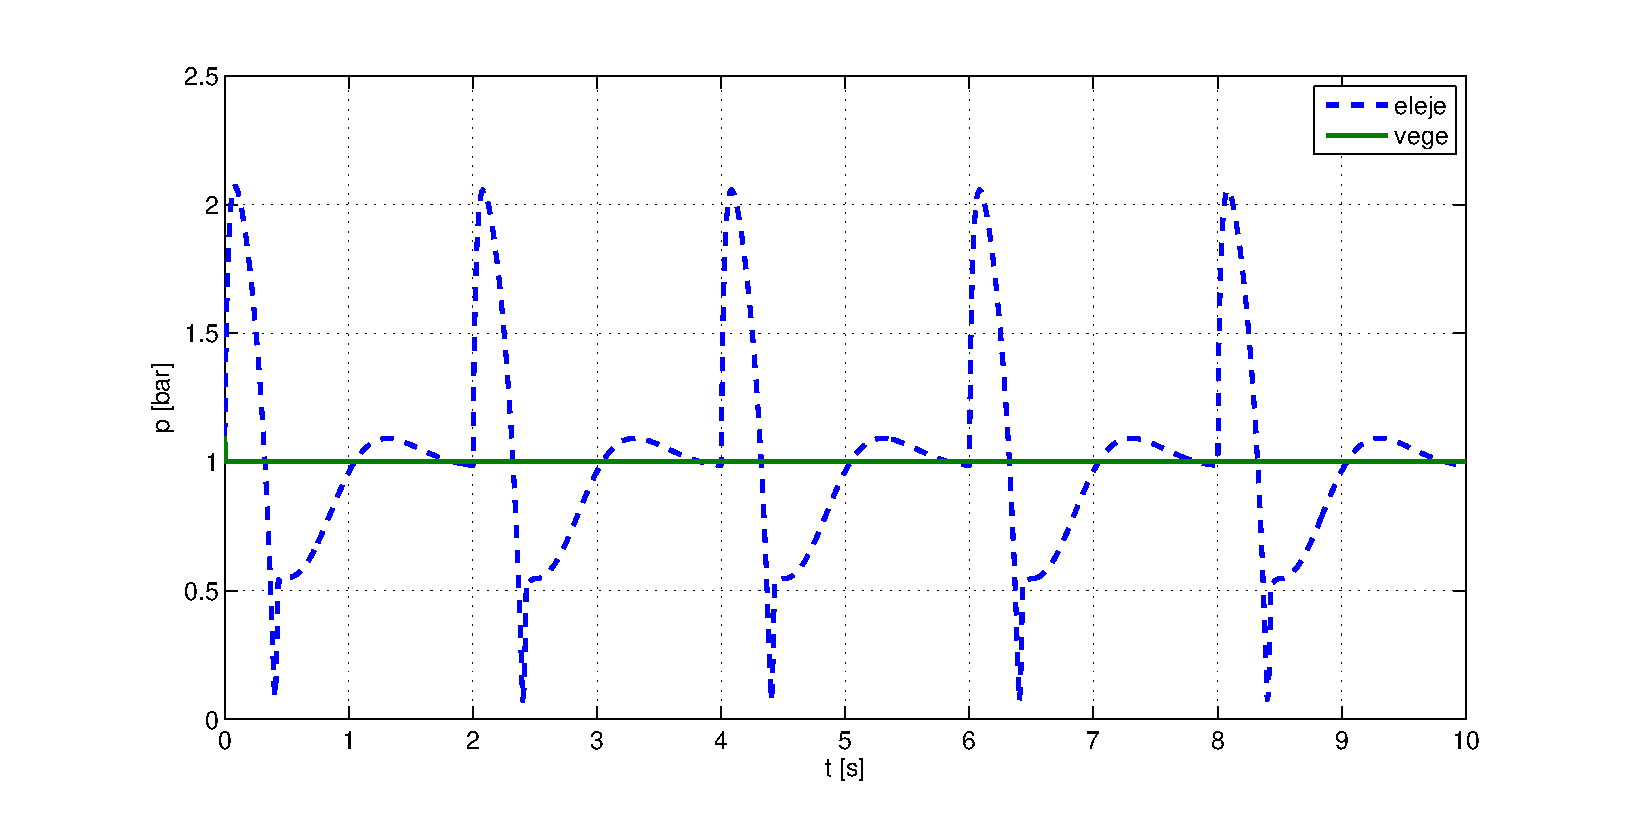
\includegraphics[width=10cm]{abrak/feladat9.eps}
    \caption{\label{9mo_abra} A 9. feladat megold�sa}
  \end{center}
\end{figure}
\vfill
%-----------------------------------
\pagebreak
%%%%%%%%%%%%%%%%%%%%%%%%%%%%%%%%%%%%
\clearpage{\pagestyle{empty}\cleardoublepage}
\chapter{A feladatok bemenetei, mint lehets�ges megold�sok}
\subsection{1.\,feladat}
\texttt{mar,medence\\
nyomas,medence,medencecsp,1000,4,3e5\\
csp,medencecsp,0,0,const}

\texttt{rugalmas\_cso,cso\\
medencecsp,csoveg,1000,4,3e5,0.15,0,5e-3,1040,2.4e9,2.2e9,10,auto,0,0\\
amoba,csoveg,0,0,const}
%---------------------------
\subsection{2.\,feladat}
\texttt{mar,medence\\
nyomas,medence,medencecsp,1000,4,3e5\\
csp,medencecsp,0,0,const}

\texttt{rugalmas\_cso,csosurl\\
medencecsp,csoveg,1000,4,3e5,0.15,0.02,5e-3,1040,2.4e9,2.2e9,10,auto,0,0\\
amoba,csoveg,0,0,const}
%---------------------------
\subsection{3.\,feladat}
\texttt{mar,also\\
nyomas,medencealso,medenceki,1000,0,1e5\\
szivattyu,szivattyu,medenceki,nyomocsp,1000,0,0.253,0.253,1,8\\
0,110,16.8\\
0.005,105,18\\
0.01,98,20.8\\
0.015,93,23.2\\
0.02,88,25.6\\
0.025,84,28\\
0.03,72,30\\
0.035,65,32\\
1450,1.9,120\\
visszacsapo\_szelep,vszelep,nyomocsp,szelepki,1000,0\\
csp,medenceki,253,0,const\\
csp,nyomocsp,253,0,const\\
csp,szelepki,253,0,const}

\texttt{mar,felso\\
nyomas,medencefelso,medencebe,1000,0,1e5\\
csp,medencebe,327,0,const}

\texttt{rugalmas\_cso,cso,szelepki,medencebe,1000,0,8.6e5,0.253,0.029,13e-3,2250,2.4e9,2.2e9,8,user\\
253,257,280,270,280,302,305,327}
%---------------------------
\subsection{4.\,feladat}
\texttt{mar,also\\
nyomas,medencealso,medenceki,1000,0,1e5\\
szivattyu,szivattyu,medenceki,nyomocsp,1000,0,0.253,0.253,1,8\\
0,110,16.8\\
0.005,105,18\\
0.01,98,20.8\\
0.015,93,23.2\\
0.02,88,25.6\\
0.025,84,28\\
0.03,72,30\\
0.035,65,32\\
1450,1.9,120\\
visszacsapo\_szelep,vszelep,nyomocsp,szelepki,1000,0\\
csp,medenceki,253,0,const\\
csp,nyomocsp,253,0,const\\
csp,szelepki,253,0,const}

\texttt{mar,fojtas\\
fojtas,tolozar,cso1vege,toloki,1000,0,111778.0695\\
csp,cso1vege,253,0,const\\
csp,toloki,253,0,const}

\texttt{mar,felso\\
nyomas,medencefelso,medencebe,1000,0,1e5\\
csp,medencebe,327,0,const}

\texttt{rugalmas\_cso,cso1,szelepki,cso1vege,1000,0,8.6e5,0.253,0.029,13e-3,1500,2.4e9,2.2e9,5,user\\
253,257,280,270,280}

\texttt{rugalmas\_cso,cso2,toloki,medencebe,1000,0,3.6e5,0.253,0.029,13e-3,750,2.4e9,2.2e9,3,user\\
302,305,327}

%------------------------------

\subsection{5.\,feladat}
\texttt{mar,also\\
nyomas,medencealso,medenceki,1000,0,1e5\\
szivattyu,szivattyu,medenceki,nyomocsp,1000,0,0.250,0.250,1,8\\
0,110,16.8\\
0.005,105,18\\
0.01,98,20.8\\
0.015,93,23.2\\
0.02,88,25.6\\
0.025,84,28\\
0.03,72,30\\
0.035,65,32\\
1450,1.9,120\\
visszacsapo\_szelep,vszelep,nyomocsp,szelepki,1000,0\\
legust,legust1,szelepki,1000,0.0,1.4,1.0,8.73e5,0.8,0.2,2\\
csp,medenceki,253,0,const\\
csp,nyomocsp,253,0,const\\
csp,szelepki,253,0,const}

\texttt{mar,felso\\
nyomas,medencefelso,medencebe,1000,0,1e5\\
csp,medencebe,327,0,const}

\texttt{rugalmas\_cso,cso,szelepki,medencebe,1000,26.72,8.73e5,0.250,0.035,13e-3,2250,2.4e9,2.2e9,8,user\\
253,257,280,270,280,302,305,327}
%-------------------------------

\subsection{6.\,feladat}
\texttt{mar,legust1\\
legust,legust1,csp1,1000,0,1.4,1,2e5,1,0,2\\
csp,csp1,0,0,const}

\texttt{mar,legust2\\
legust,legust2,csp2,1000,0,1.4,1,1e5,1,0,2\\
csp,csp2,0,0,const}

\texttt{rugalmas\_cso,cso,csp1,csp2,1000,0,0.0e5,0.3,0.1,13e-3,1000,2.1e11,2.1e9,5,auto,0,0}

%---------------------------------

\subsection{7.\,feladat}
\texttt{option,dt\_save,1.0}

\texttt{mar,alrendsz1\\
akna,ak01,csp1,1000,0,10.5,98.43,105.0,1.5,nincsrajz\\
csp,csp1,0.0,0.0,const}

\texttt{mar,alrendsz2\\
akna,ak02,csp2,1000,0,10.5,101.60,106.07,0.3,nincsrajz\\
csp,csp2,0.0,-50.0,gorbe1}

\texttt{csatorna,cs1000,csp2,csp1,1000,0.00,kor,0.4,941,102,101,0.013,0.01,1000,auto,nincsrajz,1.0}

\texttt{gorbe,gorbe1,4\\
0,1\\
600,1\\
601,0\\
1e6,0}
%-------------------------------
\subsection{8.\,feladat}
\texttt{option,dt\_save,1.0}

\texttt{mar,alrendsz1\\
akna,szt,csp1,1000,0.0,5000.0,108.0,116.0,0.2,nincsrajz\\
nyomovezetek,ny1,csp2a,csp1,1000,0.0,0.3,1402,0.015,98.6,110.52\\
szivattyu,szat01,csp2,csp2a,1000,0,0.3,0.3,5,7\\
0.0,44.4,1\\
0.028,38.1,1\\
0.052,31.3,1\\
0.075,24.4,1\\
0.087,20.5,1\\
0.103,13.9,1\\
0.115,6.9,1\\
1440,100.23,99.03,0\\
szivattyu,szat01s,csp2,csp2a,1000,0,0.3,0.3,5,7\\
0.0,44.4,1\\
0.028,38.1,1\\
0.052,31.3,1\\
0.075,24.4,1\\
0.087,20.5,1\\
0.103,13.9,1\\
0.115,6.9,1\\
1440,100.63,99.03,0\\
akna,at01,csp2,1000,0,1.5,98.43,105.22,1.5,nincsrajz\\
csp,csp1,0.0,0.0,const\\
csp,csp2,0.0,-450.0,const\\
csp,csp2a,0.0,0.0,const}

\texttt{mar,alrendsz2\\
akna,ak02,csp3,1000,0,28.3,104.60,106.07,0.4,nincsrajz\\
csp,csp3,0.0,-10.0,const}

\texttt{csatorna,cs1000,csp3,csp2,1000,0.00,kor,0.4,941,104.81,101.11,0.013,0.05,1000,auto,nincsrajz,1.0}
%-------------------------------

\subsection{9.\,feladat}
\subsubsection{,,A'' r�sz}
\texttt{option,dt\_save,auto}

\texttt{mar,alrendsz1\\
valtozo\_tomegaram,sziv01,csp1,1000,0,45\\
0,0\\
0.01,5.11875E-02\\
0.02,0.09975\\
0.03,0.145688\\
0.04,0.189\\
0.05,0.229688\\
0.06,0.26775\\
0.07,0.303188\\
0.08,0.336\\
0.09,0.366188\\
0.1,0.39375\\
0.11,0.418688\\
0.12,0.441\\
0.13,0.460688\\
0.14,0.47775\\
0.15,0.492188\\
0.16,0.504\\
0.17,0.513188\\
0.18,0.51975\\
0.19,0.523688\\
0.2,0.525\\
0.21,0.523688\\
0.22,0.51975\\
0.23,0.513188\\
0.24,0.504\\
0.25,0.492188\\
0.26,0.47775\\
0.27,0.460688\\
0.28,0.441\\
0.29,0.418688\\
0.3,0.39375\\
0.31,0.366188\\
0.32,0.336\\
0.33,0.303188\\
0.34,0.26775\\
0.35,0.229688\\
0.36,0.189\\
0.37,0.145688\\
0.38,9.975E-02\\
0.39,5.11875E-02\\
0.4,0\\
0.41,-2.55938E-02\\
0.42,-2.55938E-02\\
0.43,0\\
2.0,0\\
csp,csp1,0.0,0.0,gorbe1}

\texttt{mar,alrendsz2\\
nyomas,ny01,csp2,1000,0,1e5\\
csp,csp2,0.0,0.0,gorbe1}

\texttt{gorbe,gorbe1,2\\
0,1\\
1e6,1}

\texttt{viszkcso,vcso1,csp1,csp2,0.01,1.1e-6,0.005,5.0,0.00,1.1e5,1000,20,auto,9e6,4e5,100000,0.0,0.0}
\subsubsection{,,B'' r�sz}
\texttt{option,dt\_save,auto}

\texttt{mar,alrendsz1\\
valtozo\_tomegaram,sziv01,csp1,1000,0,file,tomegaramok.xls\\
csp,csp1,0.0,0.0,gorbe1}

\texttt{mar,alrendsz2\\
nyomas,ny01,csp2,1000,0,1e5\\
csp,csp2,0.0,0.0,gorbe1}

\texttt{gorbe,gorbe1,2\\
0,1\\
1e6,1}

\texttt{viszkcso,vcso1,csp1,csp2,0.01,1.1e-6,0.005,5.0,0.00,1.1e5,1000,20,auto,9e6,4e5,100000,0.0,0.0}
%-------------------------------
%%%%%%%%%%%%%%%%%%%%%%%%%%%%%%%%
\clearpage{\pagestyle{empty}\cleardoublepage}
%\chapter{Fejleszt�knek}

\section{Elemek}

Az oszt�lyhierarchia:

\begin{description}
\item [tranziens\_agelem:] minden merev �gelemet ebb�l kell sz�rmaztatni
	\begin{description}
	\item [tranziens\_agelem\_1csp:] 1 csom�pontos tranziens �gelemek
		\begin{description}
			\item [medence:] egyszer medence, egyenl�re m�g a szintemelked�s sincs benne...
		\end{description}
	\item [tranziens\_agelem\_2csp:] 2 csom�pontos tranziens �gelemek
		\begin{description}
			\item [konc\_cso] s�rl�d�sos teltszelv�ny� cs�
			\item [szivattyu] jellegg�rb�s szivatty�
			\item [fojtas] parabolikus jellegg�rb�j� fojt�s   
			\item [vez\_fojtas] vez�relt fojt�s
		\end{description}
	\end{description}
\item [cso:] telteszelv�ny�, elosztott param�ter�, s�rl�d�sos cs� (karakterisztik�k m�dszere)
\item [merev\_alrendszer:] merev elemekb�l �ssze�p�tett rendszer
\end{description}

\noindent Van n�h�ny olyan elj�r�s, amit mindig defini�lni kell

\begin{center}
\begin{tabular}{|l|p{7cm}|}\hline
n�v                                 & magyar�zat \\ \hline \hline
{\tt <konstruktor>}                 & az elemet l�trehoz� elj�r�s, neve az elem neve \\
{\tt out=subsref(trag,index)}       & hozz�f�r�s a mez�kh�z, pl. {\tt p1=medence1.p}\\ \hline
{\tt trag=subsasgn(trag,index,val)} & �rt�kad�s mez�knek, pl. {\tt medence1.p=1e5}\\ \hline
{\tt subsasgn(elem,flag,varargin)}  & inform�ci� k�r�s\\ \hline
\end{tabular}
\end{center}

Az {\tt info} elj�r�s {\tt flag} v�ltoz�ja mondja meg, milyen t�pu� inform�ci�t k�r�nk:

\begin{center}
\begin{tabular}{|l|l|p{8cm}|}\hline
{\tt info} & {\tt varargin}  & magyar�zat \\ \hline \hline
1          &                 & k�perny�re (parancsablakba) �ltal�nos info ( cso\-m�\-pon\-tok, v�ltoz�k, param�terek, stb... ) \\ \hline
2          & \tt{1}: f�jln�v & ugyanaz, mint az el�z�, csak f�jlba �rja.\\ \hline
3          &                 & fut�s k�zbeni info f�jlba\\ \hline
4          &                 & ????? \\ \hline
5          &                 & jellegg�rbe kirajzol�s, ha van ilyen\\ \hline
\end{tabular}
\end{center}

%%%%%%%%%%%%%%%%%%%%%%%%%%%%%%%%%%%%%%%%%%%%%%%%%%%%%%%%%%%%%%%%%%%
\pagebreak
\subsection{Rugalmas cs�vek}

A $\mathcal{C}^+$ �s $\mathcal{C}^-$ karakterisztika ment�n

\begin{equation}
\frac{d}{dt}\left( p \pm \rho a v\right) = \mp \rho g a \frac{dz}{dx} \mp \frac{\lambda}{2D} \rho a v |v| = \mathcal{K}^{\pm}.
\end{equation}

A $dy/dt \approx (y^{j+1}-y^j)/\Delta t$ k�zel�t�s�t alkalmazva az $i=2 \dots N$ bels� pontokra:

\begin{equation}
\begin{array}{lll}
\mathcal{C}^+&: \quad \left( p + \rho a v\right)_i^{j+1} &= \left( p + \rho a v\right)_{i-1}^{j} + \Delta t \mathcal{K}^+ \quad \text{�s}\\
\mathcal{C}^-&: \quad \left( p - \rho a v\right)_i^{j+1} &= \left( p - \rho a v\right)_{i+1}^{j} + \Delta t \mathcal{K}^-.
\end{array}
\end{equation}

A peremeken pedig

\begin{equation}
\begin{array}{lll}
i=N+1:& \quad \left( p - \rho a v\right)_{N+1}^{j+1} &= \left( p - \rho a v\right)_{N}^{j} + \Delta t \mathcal{K}^- \quad \text{�s}\\
i=1:  & \quad \left( p + \rho a v\right)_{1}^{j+1}   &= \left( p + \rho a v\right)_{2}^{j} + \Delta t \mathcal{K}^+.
\end{array}
\end{equation}

A peremeken �ltal�ban interpol�lni kell valamilyen $0< \delta t \leq \Delta t$ id�szintre �s az �gegyenlet egy�tthat�it kell megadni:

\begin{equation}
\begin{array}{lll}
i=1:&     \quad \left( p - \rho a v\right)_{1}^{j+1} &= \left( p - \rho a v\right)_{\delta x}^{j} + \Delta t \mathcal{K}^-_{\delta x} \quad \text{�s}\\
i=N+1:  & \quad \left( p + \rho a v\right)_{N+1}^{j+1}   &= \left( p + \rho a v\right)_{\delta x}^{j} + \Delta t \mathcal{K}^+_{\delta x},
\end{array}
\end{equation}

ahol a $*_{\delta t}$ jel�l�s azt jelenti, hogy interpol�lni kell a megfelel� $x$ helyre a $*$ v�ltoz� (nyom�s �s sebess�g) �rt�k�t. �gy az �gegyenletek egy�tthat�t a

\begin{equation}
\begin{array}{lll}
\text{a cs� elej�n:}& \quad 0=p - \frac{\rho a}{A} Q - \left( p - \rho a v\right)_{\delta x} - \Delta t \mathcal{K}^-_{\delta x} \quad \text{�s}\\
\text{a cs� v�g�n:} & \quad 0=p + \frac{\rho a}{A} Q - \left( p + \rho a v\right)_{\delta x} - \Delta t \mathcal{K}^+_{\delta x}
\end{array}
\end{equation}

egyenletekb�l tudjuk kiolvasni.
%Rugalmas cs� konstruktora k�tf�le lehet; vagy megadunk egy d�l�st ($i=dz/dx$), kezdeti nyom�st �s sebess�get, vagy csom�pontonk�nt magass�g- nyom�s- �s sebess�g�rt�keket. A 10. v�ltoz� hossza d�nti el, melyik konstrukctort v�lasztottuk.

%\begin{center}\begin{tabular}{|c||c|c|c|c|c|c|c|c|c||c|c|c|}\hline
%          &  1  &  2   &  3   &    4   &   5    &   6    &     7     &     8   &  9  & 10    &      11   &  12 \\ \hline \hline
%{\tt cso} & n�v & csp1 & csp2 & $D[m]$ & $s[m]$ & $L[m]$ & $\lambda$ & folynev & $N$ & $dz/dx$   & $p_{0,e}$ & $v_0$  \\ \hline
%{\tt cso} & n�v & csp1 & csp2 & $D[m]$ & $s[m]$ & $L[m]$ & $\lambda$ & folynev & $N$ & $h_i$ & $p_i$     & $v_i$  \\ \hline
%\end{tabular}\end{center}


\vfill

%%%%%%%%%%%%%%%%%%%%%%%%%%%%%%%%%%%%%%%%%%%%%%%%%%%%%%%%%%%%%%%%%%%
\pagebreak
\subsection{Virtu�lis elemek}

Ezeket az elemeket sosem alkalmazzuk a val�s�gban, csup�n arra val�k, hogy sz�rmaztassuk bel�l�k a val�s elemeket �s �gy egy csom� v�ltoz�t �s elj�r�st nem kell �jra meg �jra defini�lni.

\subsubsection{{\tt tranziens\_agelem}}

Kapcsol�d� mez�k �s elj�r�sok:

\begin{center}
\begin{tabular}{|l|c|l|}\hline
n�v            & default �rt�k & magyar�zat \\ \hline \hline
{\tt nev}      &   -           & n�v\\
{\tt Q}        &   -           & t�rfogat�ram, $m^3/s$\\
{\tt Qr}       &   -           & ,,r�gi'' t�rfogat�ram, $m^3/s$\\
{\tt folynev}  & {\tt viz}     & folyad�k neve\\
{\tt ro     }  & {\tt 1e3}     & s�r�s�g, $kg/m^3$\\
{\tt nu     }  & {\tt 1e-6}    & kinematikai viszkozit�s, $m^2/s$\\
{\tt mu     }  & {\tt 1e-3}    & dinamikai viszkozit�s,$Pas$\\
{\tt B      }  & {\tt 1e9}     & rugalmass�gi modulus, $Pa$\\   
{\tt resfile}  & {\tt 0}       & legyen-e kimeneti file\\ \hline
{\tt subsref}  &               & hozz�f�r�s a mez�kh�z (mind)\\
{\tt subsasgn} &               & �rt�kad�s mez�knek (mind)\\ \hline
\end{tabular}
\end{center}

\subsubsection{\tt tranziens\_agelem\_1csp}

1 csom�pontos merev �gelemek. Kapcsol�d� mez�k �s elj�r�sok:
\begin{center}
\begin{tabular}{|l|c|p{6cm}|}\hline
n�v            & default �rt�k & magyar�zat \\ \hline \hline
{\tt csp}      &      -        & kapcsol�d�si csom�pont sz�ma\\
{\tt p }       & {\tt 0}       & nyom�s a kapcsol�d�si pontban\\ \hline
{\tt subsref}  &      -        & hozz�f�r�s a mez�kh�z (mind)\\
{\tt subsasgn} &      -        & �rt�kad�s mez�knek (mind)\\
{\tt info(elem,flag,varargin)}     &               & info a mez�kr�l\\ \hline
\end{tabular}
\end{center}

\subsubsection{\tt tranziens\_agelem\_2csp}

2 csom�pontos tranziens �gelemek. Kapcsol�d� mez�k �s elj�r�sok:
\begin{center}
\begin{tabular}{|l|c|p{6cm}|}\hline
n�v            & default �rt�k & magyar�zat \\ \hline \hline
{\tt csp}      &     -         & kapcsol�d�si csom�pontok sz�ma, vektor\\
{\tt p }       & {\tt [0,0]}   & nyom�s a kapcsol�d�si csom�pontokban, vektor\\ \hline
{\tt subsref}  &               & hozz�f�r�s a mez�kh�z (mind)\\
{\tt subsasgn} &               & �rt�kad�s mez�knek (mind)\\
{\tt info(elem,flag,varargin)}     &               & info a mez�kr�l\\ \hline
\end{tabular}
\end{center}

%%%%%%%%%%%%%%%%%%%%%%%%%%%%%%%%%%%%%%%%%%%%%%%%%%%%%%%%%%%%%%%%%%%%%%%%%%%%%%%%%%%%%
\pagebreak
\subsection{Agelemek}

\subsubsection{\tt konc\_cso}

Konstruktor h�v�sa:

\begin{center}
\begin{tabular}{|c||c|c|c|c|c|c|c|c|}\hline
                &  1  &  2   &  3   &    4   &  5     &   6    &    7      & 8  \\ \hline \hline
{\tt konc\_cso} & n�v & csp1 & csp2 & $D[m]$ & $s[m]$ & $L[m]$ &  \{0.02\} & \{v�z\} \\ \hline
{\tt konc\_cso} &    &       &      &        &        &        & $\lambda$ & folyn�v \\ \hline
\end{tabular}
\end{center}


%--------------------------------
\subsubsection{\tt fojtas}

A fojt�si egyenlet alakja: $\Delta p [Pa] = K_0\, + \, K_1 \rho\, Q \left| Q \right|$, $Q[m^3/s]$. Konstruktor h�v�sa:

\begin{center}
\begin{tabular}{|c||c|c|c|c|c|c|}\hline
                &  1  &  2   &  3   &       4     &     5     &   6  \\ \hline \hline
{\tt konc\_cso} & n�v & csp1 & csp2 & $K_0[1/m^2]$ & $K_1[m^2]$ & folyn�v \\ \hline
\end{tabular}
\end{center}

%--------------------------------
\subsubsection{\tt vez\_fojtas}

A fojt�si egyenlet alakja: $\Delta p [Pa] = K_0\, + \, K_1(t) \rho\, Q \left| Q \right|$, $Q[m^3/s]$. Meg kell adni egyr�szr�l a $K_{\zeta}$ fojt�si t�nyez�t valamilyen $\varepsilon=e/D$ dimenzi�tlan geometriai param�ter f�ggv�ny�ben, pl. tol�z�r helyzet a cs��tm�r�re vonatkoztatva, ill. meg kell adni ezen geometriai param�ter id�beli v�ltoz�s�t. Teh�t adott: $t=(t_1,t_2,\dots,t_N)$ id�pontokban $\varepsilon_t=(\varepsilon_1,\varepsilon_2,\dots,\varepsilon_N)$ �s $\varepsilon_K=(\varepsilon_{t,1},\varepsilon_{t,2},\dots,\varepsilon_{t,N})$ pontokban $K_{\zeta}=(K_{\zeta,1},K_{\zeta,2} \dots K_{\zeta,N})$. A sz�m�t�s menete:
%
\begin{center}
\begin{equation*}
t\quad \Rightarrow \quad \varepsilon \quad \Rightarrow \quad K_\zeta \quad \Rightarrow \quad \zeta= \left( \frac{K}{K-1}\right)^2 \quad \Rightarrow \quad K_1=\frac{\zeta}{2\,A^2}.
\end{equation*}
\end{center}

\begin{center}
\begin{tabular}{|c||c|c|c|c|c|c|c|c|c|}\hline
                &  1  &  2   &  3   &   4     &     5    &       6         &       7     &   8  &       9  \\ \hline \hline
{\tt konc\_cso} & n�v & csp1 & csp2 & fojt.n�v & $A[m^2]$ & $(\varepsilon_K)$ & $(K_1)$  &  $(t)$ & $(\varepsilon_K)$\\ \hline
\end{tabular}
\end{center}

%--------------------------------
\subsubsection{\tt szivattyu}

A szivatty� jelleg�rb�vel rendelkezik, a konstruktor v�g�n a {\tt tranziens} kapcsol� azt mutatja, hogy milyen tranziens �llapot fog bek�vetkezni. {\tt 0} �rt�kn�l nincsen semmilyen tranziens, {\tt 1} a szivatty� kies�s, {\tt 2} �s {\tt 3} a szivatty� ind�t�s att�l f�gg�en, hogy rendelkez�se �ll-e a motor $M_m(n)$ jellegg�rb�je vagy csak az $M_b$ billen�nyomat�kot, az ahhoz tartoz� $n_b$ fordulatsz�mot �s az $n_{sz}$ szinkron fordulatsz�mot tudjuk.

\begin{center}\begin{tabular}{|c||c|c|c|c|c|c|c|c|}\hline
                &  1  &  2   &  3   &  4    &  5    &  6    &    7     & 8\\ \hline \hline
{\tt szivattyu} & n�v & csp1 & csp2 & $(Q[m^3/s])$ & $(H[m])$ & $D_s[m]$ & $D_n[m]$ & tranziens\\ \hline
\end{tabular}\end{center}

Tranziens be�ll�t�sok:

\begin{center}\begin{tabular}{|c||c|c|c|c|c|c|c|c|}\hline
                  &      9    &     10     &     11          &     12      &     13         &    14  \\ \hline \hline
{\tt tranziens=0} &           &            &                 &             &                &        \\ \hline
{\tt tranziens=1} & $(P[kW])$ & $n[1/min]$ & $\theta[kgm^2]$ & $t_{ki}[s]$ &                &        \\ \hline
{\tt tranziens=2} & $(P[kW])$ & $n[1/min]$ & $\theta[kgm^2]$ & $M_b[Nm]$   & $n_b[1/min]$   & $n_{sz}[1/min]$\\ \hline
{\tt tranziens=3} & $(P[kW])$ & $n[1/min]$ & $\theta[kgm^2]$ & $(M_m[Nm])$   & $(n_m[1/min])$ &       \\ \hline
\end{tabular}\end{center}

%%%%%%%%%%%%%%%%%%%%%%%%%%%%%%%%%%%%%%%%%%%%%%%%%%%%%%%%%%%%%%%%%%%%%%%%%%%%%%%%%%%%%
\pagebreak
\subsection{Merev alrendszer}

Merev alrendszert k�tf�lek�ppen lehet l�trehozni:
\begin{enumerate}
\item Egy {\tt fnev.dat} kiterjeszt�s� adatf�jlban fel kell sorolni az elemeket ill. a csom�pontokat, �s a konstruktor megkapja a f�jlnevet kiterjeszt�s n�lk�l. A f�jl els� sor�ban egy sz�m �ll, ami ez elemek sz�m�t jelenti, azt�n minden soronk�nt defini�lni kell az elemeket, majd a csom�pontokat: n�v, $h[m]$, $Q_{be}[m^3/s]$. pl. {\tt mar1=merev\_elrendszer('fnev')}
\item A merev alrendszer konstruktora megkapja az elemeket �s a csom�pontokat k�szen:\\ {\tt mar1=merev\_elrendszer('nev',elemek,csp)}.
\end{enumerate}

Az objektum adatmez�i:

\begin{center}
\begin{tabular}{|l|c|p{8cm}|}\hline
mez�                   &       & magyar�zat \\ \hline \hline
{\tt n\_elem}           &       & elemek sz�ma\\ \hline
{\tt n\_csp}            &       & csom�pontok sz�ma\\ \hline
{\tt elemek\{i\}}      &       & merev alrendszer elemei\\ \hline
{\tt csp\{i\} }        & \{1\} & csom�pont neve\\
{\tt csp\{i\} }        & \{2\} & csom�pont magass�ga $[m]$\\
{\tt csp\{i\} }        & \{3\} & csom�pontba befut� �gak azonos�t� sz�ma el�jelesen (vektor)\\
{\tt csp\{i\} }        & \{4\} & csom�ponti nyom�s $[Pa]$\\
{\tt csp\{i\} }        & \{5\} & elv�tel/bet�p $[m^3/s]$\\ \hline
{\tt csp\{i\} }        & \{6\} & csom�pont neve\\ \hline
\end{tabular}
\end{center}

A kimenetet szab�lyz� mez�k:
\begin{center}
\begin{tabular}{|l|c|p{9cm}|}\hline
mez�                   &       & magyar�zat \\ \hline \hline
{\tt plot\_iter}       &       & a sz�m�t�s befejez�se ut�n rajzoljuk-e ki a Newton-Raphson l�p�sek konvergenciat�rt�net�t (default:0)\\ \hline
{\tt save\_level}      &       & inform�ci� a sz�m�t�s k�zben (default:3)\\
                       &   0   & semmi\\
                       &   1   & topol�gia $\rightarrow$ {\tt fnev.out}\\
                       &   2   & topol�gia + elemek $\rightarrow$ {\tt fnev.out}\\
                       &   3   & topol�gia + elemek + eredm�nyek $\rightarrow$ {\tt fnev.out}\\
                       &   4   & topol�gia + elemek + eredm�nyek + iter�ci�k $\rightarrow$ {\tt fnev.out}\\
                       &   5   & topol�gia + elemek + eredm�nyek + iter�ci�k + m�trixok strukt�r�ja $\rightarrow$ {\tt fnev.out}\\
                       &   6   & topol�gia + elemek + eredm�nyek + iter�ci�k + m�trixok strukt�r�ja $\rightarrow$ {\tt fnev.out} �s m�trixok �rt�kei $\rightarrow$ {\tt fnev\_ABCD.res}\\ \hline

\end{tabular}
\end{center}

%%%%%%%%%%%%%%%%%%%%%%%%%%%%%%%%%%%%%%%%%%%%%%%%%%%%%%%%%%%%%%%%%%%%%%%%%%%%%%%%%%%%%
\pagebreak
\section{A f�program: {\tt eon\_driver.m}}

Az {\tt eon\_driver} elj�r�s a f�program. K�telez� param�terek a merev �s rugalmas adatf�jl �s a sz�m�t�s id�tartama, az opcion�lis param�tereket k�s�bb elsoroljuk. A szintaktika:

\begin{center}
\tt{eon\_driver(}<merev adatf�jl>,<rugalmas adatf�jl>,<id�tartam>,\{<opci�>,<�rt�k>\}\tt{)},
\end{center}

ahol az utols� blokk \{...\} t�bbsz�r is ism�tl�dhet. A lehets�ges opci�k:

\begin{center} 
\begin{tabular}{|l|c|p{9cm}|}
\emph{Opci�} & \emph{�rt�kek} & \emph{Magyar�zat} \\ \hline \hline
{\tt debug} & 0|1|2|3 & A k�perny�n fut�s k�zben megjelen� inform�ci� mennyis�ge. Alapbe�ll�t�sban 0, innen folyamatosan n� az info mennyis�ge. \\ \hline
{\tt rajz}  & 0|1     & Ha 1, a program fut�sa ut�n a rugalmas cs�vek v�gpontjain megjelen�ti a nyom�s- �s t�rfogat�ram lefut�sokat. Alapbe�ll�t�s: 0. \\ \hline
{\tt dtmin}  & <sz�m> & A megengedhet� minim�lis id�l�p�s, ami alatt �sszevonja a cs�vek id�l�p�s�t. Alapbe�ll�t�sa a legkisebb cs�-id�l�p�s ezrede.\\ \hline
{\tt op}    & windows | linux & Az oper�ci�s rendszert defini�lja, erre a fut�s eleji k�nyvt�rtiszt�t�s miatt van sz�ks�g. Alapbe�ll�t�s: windows.\\ \hline
\end{tabular}
\end{center}

P�ld�k futtat�sra {\tt Matlab} k�rnyezetben:

\begin{description}
\item[{\tt eon\_driver('f0','f0',20)}]  $\Rightarrow$ merev adatf�jl: {\tt f0.mdt}, rugalmas adatf�jl: {\tt f0.dat}, id�tartam: $20s$.
\item[{\tt eon\_driver('f0','f0',20,'debug',2)}] $\Rightarrow$ t�bb inform�ci� a k�perny�re.
\item[{\tt eon\_driver('f0','f0',20,'debug',2,'op','linux')}] $\Rightarrow$ futtat�s Linux op. rendszer alatt.
\end{description}

A program f� r�szei: (1) merev alrendszerek fel�p�t�s: {\tt olvas5m.m} h�v�sa, (2) rugalmas alrendszerek �p�t�se: {\tt olvas5r.m} h�v�sa, (3) rugalmas �s merev alrendszerek csatlakoz�s�nak fel�p�t�se, (4) sz�m�t�s �s (5) eredm�nyek list�z�sa. A f�jl v�g�n k�l�n elj�r�s az id�l�p�s v�laszt�s�t elv�gz� {\tt dtuj} elj�r�s.

A fut�s k�zben haszn�lt bels� adatstrukt�r�k, melyek a topol�gi�t �rj�k le:

\begin{itemize}
\item {\tt mar\{i\}, i=1..n\_mar} A merev alrendszereket tartalmaz� vektor. Az {\tt olvas5m.m} elj�r�s kimenete.
\item {\tt csovek\{i\}, i=1..n\_cso} A rugalmas cs�veket tartalmaz vektor. Az {\tt olvas5r.m} elj�r�s kimenete.
\end{itemize}

{\bf Csom�pont Biblia:} {\tt cspb} objektum

Ez a strukt�ra tartalmazza az �sszes merev alrendszer �sszes csom�pontj�t. Minden eleme ({\tt cspb\{i\}}) egy csom�pontnak felel meg:

\begin{center}
\begin{tabular}{|l|c|p{8cm}|}
\emph{Mez�}             &       & \emph{Magyar�zat} \\ \hline \hline
{\tt cspb\{i\} }        & \{1\} & Merev alrendszer sz�ma.\\ \hline
{\tt cspb\{i\} }        & \{2\} & Merev alrendszerben a csom�pont sz�ma. \\ \hline
{\tt cspb\{i\} }        & \{3\} & A csom�pont neve. \\ \hline
\end{tabular}
\end{center}

{\bf Topol�gia nyilv�ntart�sa}

A {\tt tjcs } m�trix minden egyes sora megfelel egy 'glob�lis' csom�pontnak, azaz egy olyan csom�pontnak, ahol merev-rugalmas vagy rugalmas-rugalmas kapcsol�d�s van. Az els� {\tt n\_cso} sz�m� oszlop a rugalmas cs�veket reprezent�lja. Ha az i-edik csom�pontb�l indul a j-edik rugalmas cs�, {\tt t(i,j)=-1}, ha onnan indul {\tt t(i,j)=1}. Az els� {\tt n\_cso} sz�m� oszlop ut�n k�vetkez� {n\_mar} oszlop a merev alrendszerekkel val� kapcsol�d�st mutatja. Ha az i-edik glob�lis csom�pont a j-edik merev alrendszer \emph{bels�} sz�moz�s�ban k, akkor {\tt tjcs(i,n\_cso+j)=k}. Ha egy glob�lis csom�pont am�ba, azaz rugalmas-rugalmas kapcsol�d�sr�l van sz�, a merev alrendszerek oszlopaiban csupa z�rus elem �ll.

\begin{figure}[h]
  \begin{center}
    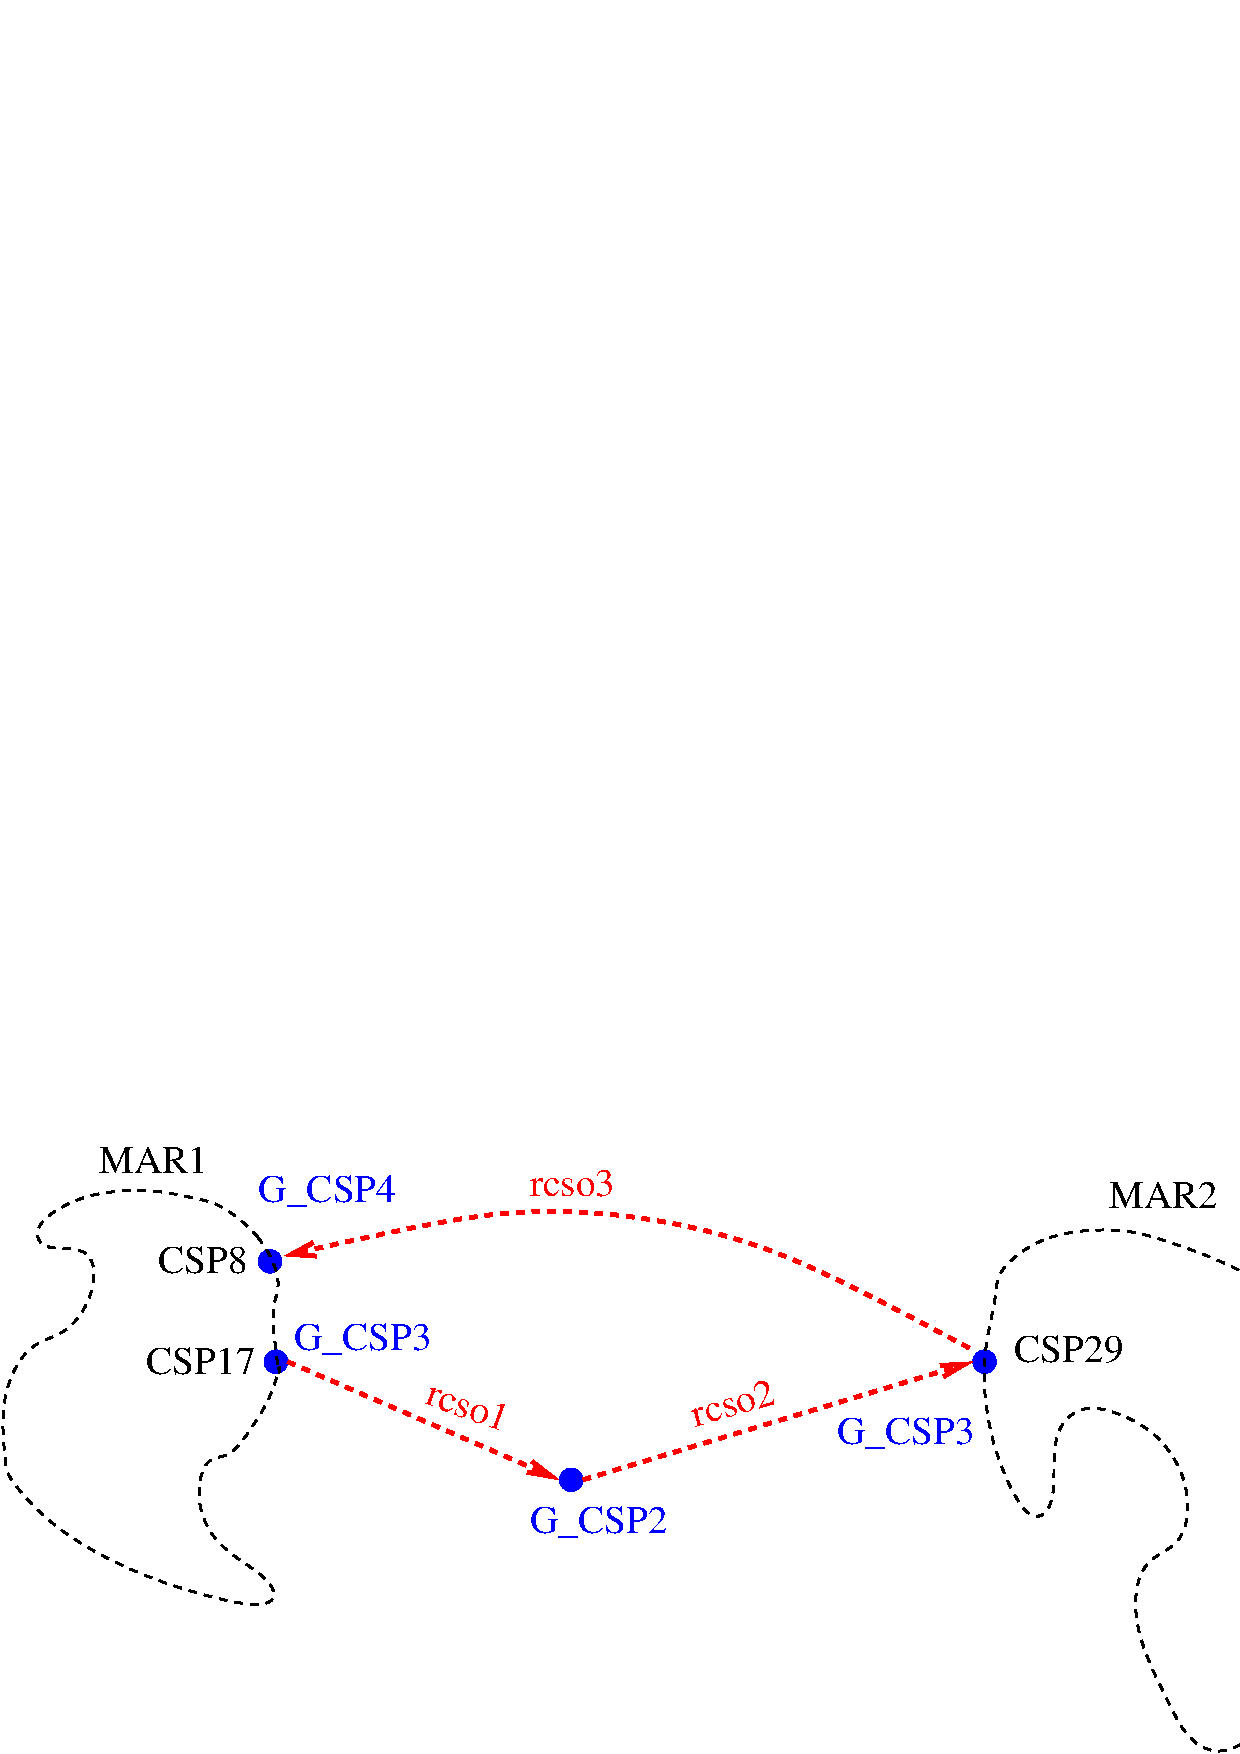
\includegraphics[width=12cm]{abrak/top_pelda.pdf}
%    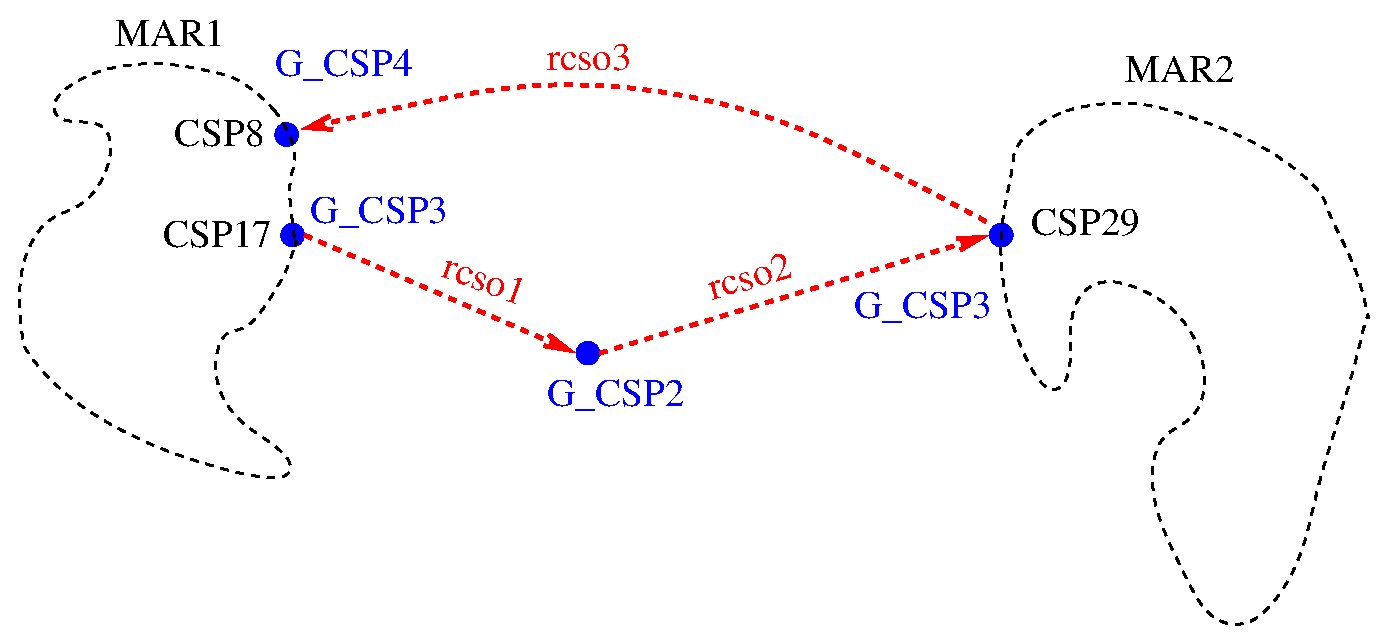
\includegraphics[width=12cm]{abrak/top_pelda.eps}
    \caption{\label{top_pelda} P�lda topol�ig�ra, a megfelel� {\tt tjcs} m�trix a \ref{top_pelda_tablazat}. t�bl�zatban l�that�.}
  \end{center}
\end{figure}

\begin{table}[h]
  \begin{center}
    \begin{tabular}{c||ccc|cc|}
             & rcso1 & rcso2 & rcso3 & mar1 & mar2\\ \hline \hline
      g\_csp1 & -1    & 0     & 0     & 17   & 0 \\ \hline
      g\_csp2 & 1     & -1    & 0     & 0    & 0 \\ \hline
      g\_csp3 & 0     &  1    & -1    & 0    & 29 \\ \hline
      g\_csp4 & 0     &  0    & 1     & 8    & 0 \\ \hline
    \end{tabular}
    \caption{\label{top_pelda_tablazat} Topol�gia p�lda.}
  \end{center}
\end{table}

A {\tt tjcs} �p�t�se k�zben felt�lt�dik egy {\tt gcsp\_tipus} (glob�lis csom�pont t�pus) vektor is, aminek i-edik eleme 1, ha az i-edik glob�lis csom�pont merev-rugalmas csatlakoz�s �s 2, ha am�ba (rugalmas-rugalmas)\footnote{Az adatf�jlokon kereszt�l m�g nem el�rhet� ugyan, de van egy 3. lehet�s�g, amikor adott nyom�s� am�ba csom�pontr�l van sz�, ekkor a megfelel� elem 3.}.

Ezeken k�v�l a h�l�zat fel�p�t�se ut�n l�trehozunk egy {\tt cso\_mar} �s egy {\tt mar\_cso} nev� objektumot, ezek a futtat�s k�zben hasznosak. A {\tt cso\_mar{i}} strukt�ra k�t mez�b�l �ll, mind a k�t mez� egy-egy vektort tartalmaz. Az els� elem a cs� elej�re, a m�sodik a cs� v�g�re vonatkozik, a vektorok pedig a kapcsol�d� merev alrendszer sz�m�t �s a csom�pontsz�mot tartalmazz�k. A fenti p�ld�ban {\tt mar\_cso{1}{1}=[1,17]}, {\tt mar\_cso{1}{2}=[0,0]}, {\tt mar\_cso{2}{1}=[0,0]}, {\tt mar\_cso{2}{2}=[2,29]}, {\tt mar\_cso{3}{1}=[2,29]}, {\tt mar\_cso{3}{2}=[1,17]}. A m�sik strukt�ra a merev alrendszerek friss�t�sekor megmutatja, hogy honnan van sz�ks�g peremfelt�telekre, ennek merev alrendszerenk�nt annyi mez�je van, ah�ny rugalmas cs�h�z kapcsol�d� csom�pontja van a merev alrendszernek. Az utols� k�t mez� pedig megadja a kapcsol�d� csom�pont bels� sz�m�t ill. a hozz� kapcsol�d� rugalmas cs�vek sz�m�t el�jelesen (az indul� rugalmas cs�vek negat�v el�jel�ek, az �rkez�k pozit�vak). A fenti p�ld�ban {\tt mar\_cso{1}{1}{1}=17}, {\tt mar\_cso{1}{1}{2}=[-1]}, {\tt mar\_cso{1}{2}{1}=8}, {\tt mar\_cso{1}{2}{2}=[3]}, {\tt mar\_cso{2}{1}{1}=29} �s {\tt mar\_cso{2}{1}{2}=[2,-3]}.












\chapter{Fejleszt�knek}

\section{Elemek}

Az oszt�lyhierarchia:

\begin{description}
\item [tranziens\_agelem:] minden merev �gelemet ebb�l kell sz�rmaztatni
	\begin{description}
	\item [tranziens\_agelem\_1csp:] 1 csom�pontos tranziens �gelemek
		\begin{description}
			\item [medence:] egyszer medence, egyenl�re m�g a szintemelked�s sincs benne...
		\end{description}
	\item [tranziens\_agelem\_2csp:] 2 csom�pontos tranziens �gelemek
		\begin{description}
			\item [konc\_cso] s�rl�d�sos teltszelv�ny� cs�
			\item [szivattyu] jellegg�rb�s szivatty�
			\item [fojtas] parabolikus jellegg�rb�j� fojt�s   
			\item [vez\_fojtas] vez�relt fojt�s
		\end{description}
	\end{description}
\item [cso:] telteszelv�ny�, elosztott param�ter�, s�rl�d�sos cs� (karakterisztik�k m�dszere)
\item [merev\_alrendszer:] merev elemekb�l �ssze�p�tett rendszer
\end{description}

\noindent Van n�h�ny olyan elj�r�s, amit mindig defini�lni kell

\begin{center}
\begin{tabular}{|l|p{7cm}|}\hline
n�v                                 & magyar�zat \\ \hline \hline
{\tt <konstruktor>}                 & az elemet l�trhoz� elj�r�s, neve az elem neve \\
{\tt out=subsref(trag,index)}       & hozz�f�r�s a mez�kh�z, pl. {\tt p1=medence1.p}\\ \hline
{\tt trag=subsasgn(trag,index,val)} & �rt�kad�s mez�knek, pl. {\tt medence1.p=1e5}\\ \hline
{\tt subsasgn(elem,flag,varargin)}  & inform�ci� k�r�s\\ \hline
\end{tabular}
\end{center}

Az {\tt info} elj�r�s {\tt flag} v�ltoz�ja mondja meg, milyen t�pu� inform�ci�t k�r�nk:

\begin{center}
\begin{tabular}{|l|l|p{8cm}|}\hline
{\tt info} & {\tt varargin}  & magyar�zat \\ \hline \hline
1          &                 & k�perny�re (parancsablakba) �ltal�nos info ( cso\-m�\-pon\-tok, v�ltoz�k, param�terek, stb... ) \\ \hline
2          & \tt{1}: filen�v & ugyanaz, mint az el�z�, csak file-ba �rja.\\ \hline
3          &                 & fut�s k�zbeni info fileba\\ \hline
4          &                 & ????? \\ \hline
5          &                 & jellegg�rbe plottol�s, ha van ilyen\\ \hline
\end{tabular}
\end{center}

\subsection{Virtu�lis elemek}

Ezeket az elemeket sosem alkalmazzuk a val�s�gban, csup�n arra val�k, hogy sz�rmaztassuk bel�l�k a val�s elemeket �s �gy egy csom� v�ltoz�t �s elj�r�st nem kell �jra meg �jra defini�lni.

\subsubsection{{\tt tranziens\_agelem}}

Kapcsol�d� mez�k �s elj�r�sok:

\begin{center}
\begin{tabular}{|l|c|l|}\hline
n�v            & default �rt�k & magyar�zat \\ \hline \hline
{\tt nev}      &   -           & n�v\\
{\tt Q}        &   -           & t�rfogat�ram, $m^3/s$\\
{\tt Qr}       &   -           & ``r�gi'' t�rfogat�ram, $m^3/s$\\
{\tt folynev}  & {\tt viz}     & folyad�k neve\\
{\tt ro     }  & {\tt 1e3}     & s�r�s�g, $kg/m^3$\\
{\tt nu     }  & {\tt 1e-6}    & kinematikai viszkozit�s, $m^2/s$\\
{\tt mu     }  & {\tt 1e-3}    & dinamikai viszkozit�s,$Pas$\\
{\tt B      }  & {\tt 1e9}     & rugalmass�gi modulus, $Pa$\\   
{\tt resfile}  & {\tt 0}       & legyen-e kimeneti file\\ \hline
{\tt subsref}  &               & hozz�f�r�s a mez�kh�z (mind)\\
{\tt subsasgn} &               & �rt�kad�s mez�knek (mind)\\ \hline
\end{tabular}
\end{center}

\subsubsection{\tt tranziens\_agelem\_1csp}

1 csom�pontos merev �gelemek. Kapcsol�d� mez�k �s elj�r�sok:
\begin{center}
\begin{tabular}{|l|c|p{6cm}|}\hline
n�v            & default �rt�k & magyar�zat \\ \hline \hline
{\tt csp}      &      -        & kapcsol�d�si csom�pont sz�ma\\
{\tt p }       & {\tt 0}       & nyom�s a kapcsol�d�si pontban\\ \hline
{\tt subsref}  &      -        & hozz�f�r�s a mez�kh�z (mind)\\
{\tt subsasgn} &      -        & �rt�kad�s mez�knek (mind)\\
{\tt info(elem,flag,varargin)}     &               & info a mez�kr�l\\ \hline
\end{tabular}
\end{center}

\subsubsection{\tt tranziens\_agelem\_2csp}

2 csom�pontos tranziens �gelemek. Kapcsol�d� mez�k �s elj�r�sok:
\begin{center}
\begin{tabular}{|l|c|p{6cm}|}\hline
n�v            & default �rt�k & magyar�zat \\ \hline \hline
{\tt csp}      &     -         & kapcsol�d�si csom�pontok sz�ma, vektor\\
{\tt p }       & {\tt [0,0]}   & nyom�s a kapcsol�d�si csom�pontokban, vektor\\ \hline
{\tt subsref}  &               & hozz�f�r�s a mez�kh�z (mind)\\
{\tt subsasgn} &               & �rt�kad�s mez�knek (mind)\\
{\tt info(elem,flag,varargin)}     &               & info a mez�kr�l\\ \hline
\end{tabular}
\end{center}

\subsection{Agelemek}

\subsubsection{\tt konc\_cso}

Konstruktor h�v�sa:

\begin{center}
\begin{tabular}{|c||c|c|c|c|c|c|c|c|}\hline
                &  1  &  2   &  3   &    4   &  5     &   6    &    7      & 8  \\ \hline \hline
{\tt konc\_cso} & n�v & csp1 & csp2 & $D[m]$ & $s[m]$ & $L[m]$ &  \{0.02\} & \{v�z\} \\ \hline
{\tt konc\_cso} &    &       &      &        &        &        & $\lambda$ & folyn�v \\ \hline
\end{tabular}
\end{center}

%--------------------------------
\subsubsection{\tt fojtas}

A fojt�si egyenlet alakja: $\Delta p [Pa] = K_0\, + \, K_1 \rho\, Q \left| Q \right|$, $Q[m^3/s]$. Konstruktor h�v�sa:

\begin{center}
\begin{tabular}{|c||c|c|c|c|c|c|}\hline
                &  1  &  2   &  3   &       4     &     5     &   6  \\ \hline \hline
{\tt konc\_cso} & n�v & csp1 & csp2 & $K_0[1/m^2]$ & $K_1[m^2]$ & folyn�v \\ \hline
\end{tabular}
\end{center}

%--------------------------------
\subsubsection{\tt vez\_fojtas}

A fojt�si egyenlet alakja: $\Delta p [Pa] = K_0\, + \, K_1(t) \rho\, Q \left| Q \right|$, $Q[m^3/s]$. Meg kell adni egyr�szr�l a $K_{\zeta}$ fojt�si t�nyez�t valamilyen $\varepsilon=e/D$ dimenzi�tlan geometriai param�ter f�ggv�ny�ben, pl. tol�z�r helyzet a cs��tm�r�re vonatkoztatva, ill meg kell adni ezen geometriai param�ter id�beli v�ltoz�s�t. Teh�t adott: $t=(t_1,t_2,\dots,t_N)$ id�pontokban $\varepsilon_t=(\varepsilon_1,\varepsilon_2,\dots,\varepsilon_N)$ �s $\varepsilon_K=(\varepsilon_{t,1},\varepsilon_{t,2},\dots,\varepsilon_{t,N})$ pontokban $K_{\zeta}=(K_{\zeta,1},K_{\zeta,2} \dots K_{\zeta,N})$. A sz�m�t�s menete:
%
\begin{center}
\begin{equation*}
t\quad \Rightarrow \quad \varepsilon \quad \Rightarrow \quad K_\zeta \quad \Rightarrow \quad \zeta= \left( \frac{K}{1-K}\right)^2 \quad \Rightarrow \quad K_1=\frac{\zeta}{2\,A^2}.
\end{equation*}
\end{center}

\begin{center}
\begin{tabular}{|c||c|c|c|c|c|c|c|c|c|}\hline
                &  1  &  2   &  3   &   4     &     5    &       6         &       7     &   8  &       9  \\ \hline \hline
{\tt konc\_cso} & n�v & csp1 & csp2 & folyn�v & $A[m^2]$ & $(\varepsilon_K)$ & $(K_1)$  &  $(t)$ & $(\varepsilon_K)$\\ \hline
\end{tabular}
\end{center}

%--------------------------------
\subsubsection{\tt szivattyu}

A szivatty� jelleg�rb�vel rendelkezik, a konstruktor v�g�n a {\tt tranziens} kapcsol� azt mutatja, hogy milyen tranziens �llapot fog bek�vetkezni. {\tt 0} �rt�kn�l nincsen semmilyen tranziens, {\tt 1} a szivatty� kies�s, {\tt 2} �s {\tt 3} a szivatty� ind�t�s att�l f�gg�en, hogy rendelkez�se �ll-e a motor $M_m(n)$ jellegg�rb�je vagy csak az $M_b$ billen�nyomat�kot, az ahhoz tartoz� $n_b$ forulatsz�mot �s az $n_{sz}$ szinkron forulatsz�mot tudjuk.

\begin{center}\begin{tabular}{|c||c|c|c|c|c|c|c|c|}\hline
                &  1  &  2   &  3   &  4    &  5    &  6    &    7     & 8\\ \hline \hline
{\tt szivattyu} & n�v & csp1 & csp2 & $(Q[m^3/s])$ & $(H[m])$ & $D_s[m]$ & $D_n[m]$ & tranziens\\ \hline
\end{tabular}\end{center}

Tranziens be�ll�t�sok:

\begin{center}\begin{tabular}{|c||c|c|c|c|c|c|c|c|}\hline
                  &      9    &     10     &     11          &     12      &     13         &    14  \\ \hline \hline
{\tt tranziens=0} &           &            &                 &             &                &        \\ \hline
{\tt tranziens=1} & $(P[kW])$ & $n[1/min]$ & $\theta[kgm^2]$ & $t_{ki}[s]$ &                &        \\ \hline
{\tt tranziens=2} & $(P[kW])$ & $n[1/min]$ & $\theta[kgm^2]$ & $M_b[Nm]$   & $n_b[1/min]$   & $n_{sz}[1/min]$\\ \hline
{\tt tranziens=3} & $(P[kW])$ & $n[1/min]$ & $\theta[kgm^2]$ & $(M_m[Nm])$   & $(n_m[1/min])$ &       \\ \hline
\end{tabular}\end{center}

\subsection{Merev alrendszer}

Merev alrendszert k�tf�lek�ppen lehet l�trehozni:
\begin{enumerate}
\item Egy {\tt fnev.dat} kiterjeszt�s� adatfileban fel kell sorolni az elemeket ill. a csom�pontokat, �s a konstruktor megkapja a filenevet kiterjeszt�s n�lk�l. A file els� sor�ban egy sz�m �ll, ami ez elemek sz�m�t jelenti, azt�n minden soronk�nt defini�lni kell az elemeket, majd a csom�pontokat: n�v, $h[m]$, $Q_{be}[m^3/s]$. pl. {\tt mar1=merev\_elrendszer('fnev')}
\item A merev elrendszer konstruktora megkapja az elemeket �s a csom�pontokat k�szen:\\ {\tt mar1=merev\_elrendszer('nev',elemek,csp)}.
\end{enumerate}

Az objektum adatmez�i:

\begin{center}
\begin{tabular}{|l|c|p{8cm}|}\hline
mez�                   &       & magyar�zat \\ \hline \hline
{\tt n\_elem}           &       & elemek sz�ma\\ \hline
{\tt n\_csp}            &       & csom�pontok sz�ma\\ \hline
{\tt elemek\{i\}}      &       & merev alrendszer elemei\\ \hline
{\tt csp\{i\} }        & \{1\} & csom�pont neve\\
{\tt csp\{i\} }        & \{2\} & csom�pont magass�ga $[m]$\\
{\tt csp\{i\} }        & \{3\} & csom�pontba befut� �gak azonos�t� sz�ma el�jelesen (vektor)\\
{\tt csp\{i\} }        & \{4\} & csom�ponti nyom�s $[Pa]$\\
{\tt csp\{i\} }        & \{5\} & elv�tel/bet�p $[m^3/s]$\\ \hline
{\tt csp\{i\} }        & \{6\} & csom�pont neve\\ \hline
\end{tabular}
\end{center}

A kimenetet szab�lyz� mez�k:
\begin{center}
\begin{tabular}{|l|c|p{9cm}|}\hline
mez�                   &       & magyar�zat \\ \hline \hline
{\tt plot\_iter}       &       & a sz�m�t�s befejez�se ut�n rajzoljuk-e ki a Newton-Raphson l�p�sek konvergenciat�rt�net�t (default:0)\\ \hline
{\tt save\_level}      &       & inform�ci� a sz�m�t�s k�zben (default:3)\\
                       &   0   & semmi\\
                       &   1   & topol�gia $\rightarrow$ {\tt fnev.out}\\
                       &   2   & topol�gia + elemek $\rightarrow$ {\tt fnev.out}\\
                       &   3   & topol�gia + elemek + eredm�nyek $\rightarrow$ {\tt fnev.out}\\
                       &   4   & topol�gia + elemek + eredm�nyek + iter�ci�k $\rightarrow$ {\tt fnev.out}\\
                       &   5   & topol�gia + elemek + eredm�nyek + iter�ci�k + m�trixok strukt�r�ja $\rightarrow$ {\tt fnev.out}\\
                       &   6   & topol�gia + elemek + eredm�nyek + iter�ci�k + m�trixok strukt�r�ja $\rightarrow$ {\tt fnev.out} �s m�trixok �rt�kei $\rightarrow$ {\tt fnev\_ABCD.res}\\ \hline

\end{tabular}
\end{center}
%%%%%%%%%%%%%%%%%%%%%%%%%%%%%%%%%%%%%%%%%%%%%%%%%%%%%%%%%%%%%%%%%%%%%%%%%%%%%%%%%%%%%
\subsection{Rugalmas cs�vek}

Rugalmas cs� konstruktora k�tf�le lehet; vagy megadunk egy d�l�st ($i=dz/dx$), kezdeti nyom�st �s sebess�get, vagy csom�pontonk�nt magass�g- nyom�s- �s sebess�g�rt�keket. A 10. v�ltoz� hossza d�nti el, melyik konstrukctort v�lasztottuk.

\begin{center}\begin{tabular}{|c||c|c|c|c|c|c|c|c|c||c|c|c|}\hline
          &  1  &  2   &  3   &    4   &   5    &   6    &     7     &     8   &  9  & 10    &      11   &  12 \\ \hline \hline
{\tt cso} & n�v & csp1 & csp2 & $D[m]$ & $s[m]$ & $L[m]$ & $\lambda$ & folynev & $N$ & $dz/dx$   & $p_{0,e}$ & $v_0$  \\ \hline
{\tt cso} & n�v & csp1 & csp2 & $D[m]$ & $s[m]$ & $L[m]$ & $\lambda$ & folynev & $N$ & $h_i$ & $p_i$     & $v_i$  \\ \hline
\end{tabular}\end{center}

\section{A f�program: {\tt eon\_driver.m}}

Az {\tt eon\_driver} elj�r�s a f�program. K�telez� param�terek a merev �s rugalmas adaf�jl �s a sz�m�t�s id�tartama, az opcion�lis param�tereket k�s�bb elsoroljuk. A szintaktika:

\begin{center}
\tt{eon\_driver(}<merev adaf�jl>,<rugalmas adaf�jl>,<id�tartam>,\{<opci�>,<�rt�k>\}\tt{)},
\end{center}

ahol az utols� blokk \{...\} t�bbsz�r is ism�tl�dhet. A lehets�ges opci�k:

\begin{center} 
\begin{tabular}{|l|c|p{9cm}|}
\emph{Opci�} & \emph{�rt�kek} & \emph{Magyar�zat} \\ \hline \hline
{\tt debug} & 0|1|2|3 & A k�perny�n fut�s k�zben megjelen� inform�ci� mennyis�ge. Alapbe�ll�t�sban 0, innen folyamatosan n� az info mennyis�ge. \\ \hline
{\tt rajz}  & 0|1     & Ha 1, a program fut�sa ut�n a rugalmas cs�vek v�gpontjain megjelen�ti a nyom�s- �s t�rfogat�ram lefut�sokat. Alapbe�ll�t�s: 0. \\ \hline
{\tt dtmin}  & <sz�m> & A megengedhet� minim�lis id�l�p�s, ami alatt �sszevonja a cs�vek id�l�p�s�t. Alapbe�ll�t�sa a legkisebb cs�-id�l�p�s ezrede.\\ \hline
{\tt op}    & windows | linux & Az oper�ci�s rendszert defini�lja, erre a fut�s eleji k�nyvt�rtiszt�t�s miatt van sz�ks�g. Alapbe�ll�t�s: windows.\\ \hline
\end{tabular}
\end{center}

P�ld�k futtat�sra {\tt Matlab} k�rnyezetben:

\begin{description}
\item[{\tt eon\_driver('f0','f0',20)}]  $\Rightarrow$ merev adatf�jl: {\tt f0.mdt}, rugalmas adaf�jl: {\tt f0.dat}, id�tartam: $20s$.
\item[{\tt eon\_driver('f0','f0',20,'debug',2)}] $\Rightarrow$ t�bb inform�ci� a k�perny�re.
\item[{\tt eon\_driver('f0','f0',20,'debug',2,'op','linux')}] $\Rightarrow$ futtat�s Linux op. rendszer alatt.
\end{description}

A program f� r�szei: (1) merev alrendszerek fel�p�t�s: {\tt olvas5m.m} h�v�sa, (2) rugalmas alrendszerek �p�t�se: {\tt olvas5r.m} h�v�sa, (3) rugalmas �s merev alrendszerek csatlakoz�s�nak fel�p�t�se, (4) sz�m�t�s �s (5) eredm�nyek list�z�sa. A f�jl v�g�n k�l�n elj�r�s az id�l�p�s v�laszt�s�t elv�gz� {\tt dtuj} elj�r�s.

A fut�s k�zben haszn�lt bels� adatstrukt�r�k, melyek a topol�gi�t �rj�k le:

\begin{itemize}
\item {\tt mar\{i\}, i=1..n\_mar} A merev alrendszereket tartalmaz� vektor. Az {\tt olvas5m.m} eljaras kimenete.
\item {\tt csovek\{i\}, i=1..n\_cso} A rugalmas cs�veket tartalmaz vektor. Az {\tt olvas5r.m} eljaras kimenete.
\end{itemize}

{\bf Csom�pont Biblia:} {\tt cspb} objektum

Ez a strukt�ra tartalmazza az �sszes merev alrendszer �sszes csom�pontj�t. Minden eleme ({\tt cspb\{i\}}) egy csom�pontnak felel meg:

\begin{center}
\begin{tabular}{|l|c|p{8cm}|}
\emph{Mez�}             &       & \emph{Magyar�zat} \\ \hline \hline
{\tt cspb\{i\} }        & \{1\} & Merev alrendszer sz�ma.\\ \hline
{\tt cspb\{i\} }        & \{2\} & Merev alrendszerben a csom�pont sz�ma. \\ \hline
{\tt cspb\{i\} }        & \{3\} & A csom�pont neve. \\ \hline
\end{tabular}
\end{center}

{\bf Topol�gia nyilv�ntart�sa}

A {\tt tjcs } m�trix minden egyes sora megfelel egy 'glob�lis' csom�pontnak, azaz egy olyan csom�pontnak, ahol merev-rugalmas vagy rugalmas-rugalmas kapcsol�d�s van. Az els� {\tt n\_cso} sz�m� oszlop a rugalmas cs�veket reprezent�lja. Ha az i-edik csom�pontb�l indul a j-edik rugalmas cs�, {\tt t(i,j)=-1}, ha onnan indul {\tt t(i,j)=1}. Az els� {\tt n\_cso} sz�m� oszlop ut�n k�vetkez� {n\_mar} oszlop a merev alrendszerekkel val� kapcsol�d�st mutatja. Ha az i-edik glob�lis csom�pont a j-edik merev alrendszer \emph{bels�} sz�moz�s�ban k, akkor {\tt tjcs(i,n\_cso+j)=k}. Ha egy glob�lis csom�pont am�ba, azaz rugalmas-rugalmas kapcsol�d�sr�l van sz�, a merev alrendszerek oszlopaiban csupa z�rus elem �ll.

\begin{figure}[ht!]
  \begin{center}
    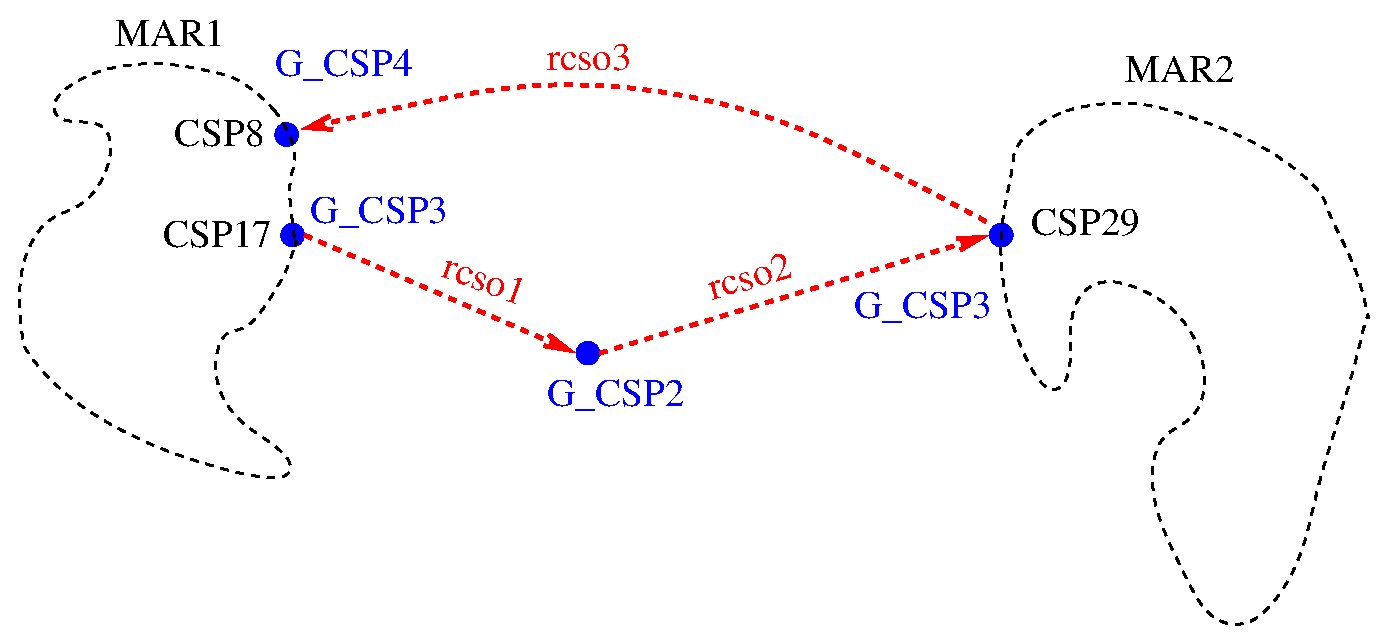
\includegraphics[width=12cm]{abrak/top_pelda}
%    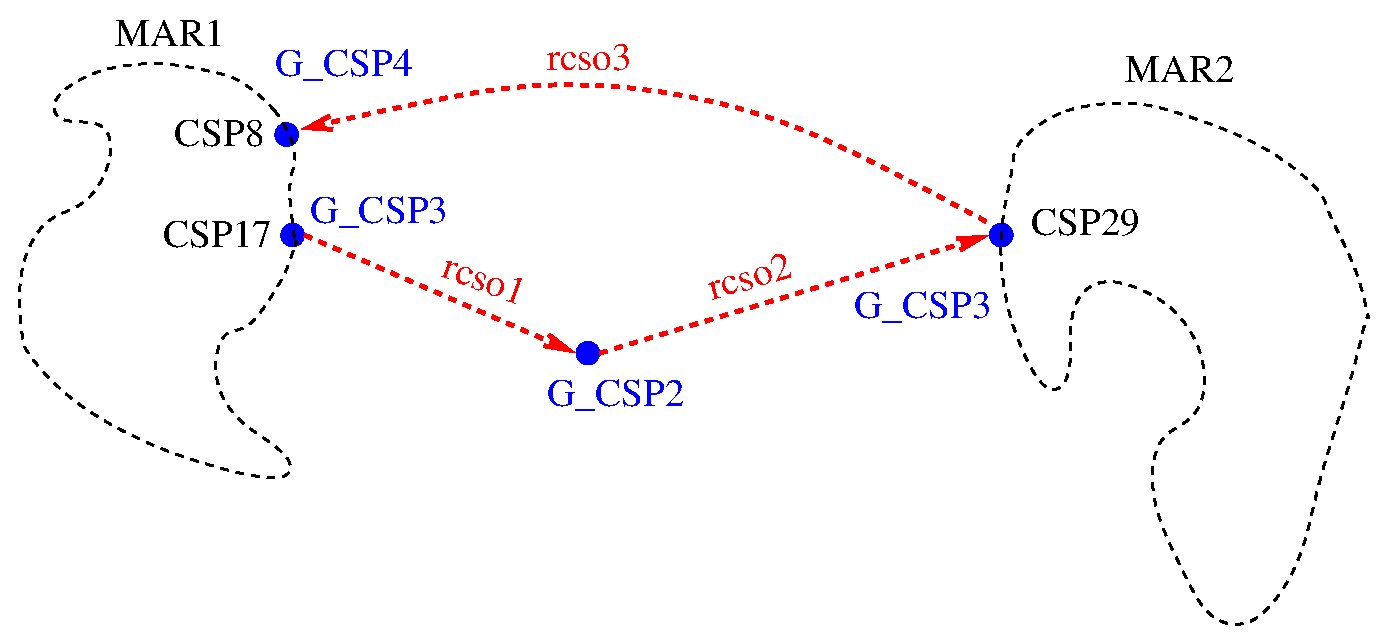
\includegraphics[width=12cm]{abrak/top_pelda.eps}
    \caption{\label{top_pelda} P�lda topol�ig�ra, a megfelel� {\tt tjcs} m�trix a \ref{top_pelda_tablazat}. t�bl�zatban l�that�.}
  \end{center}
\end{figure}

\begin{table}[ht!]
  \begin{center}
    \begin{tabular}{c||ccc|cc|}
             & rcso1 & rcso2 & rcso3 & mar1 & mar2\\ \hline \hline
      g\_csp1 & -1    & 0     & 0     & 17   & 0 \\ \hline
      g\_csp2 & 1     & -1    & 0     & 0    & 0 \\ \hline
      g\_csp3 & 0     &  1    & -1    & 0    & 29 \\ \hline
      g\_csp4 & 0     &  0    & 1     & 8    & 0 \\ \hline
    \end{tabular}
    \caption{\label{top_pelda_tablazat} Topol�gia p�lda.}
  \end{center}
\end{table}

A {\tt tjcs} �p�t�se k�zben felt�lt�dik egy {\tt gcsp\_tipus} (glob�lis csom�pont t�pus) vektor is, aminek i-edik eleme 1, ha az i-edik glob�lis csom�pont merev-rugalmas csatlakoz�s �s 2, ha am�ba (rugalmas-rugalmas)\footnote{Az adatf�jlokon kereszt�l m�g nem el�rhet� ugyan, de van egy 3. lehet�s�g, amikor adott nyom�s� am�ba csom�pontr�l van sz�, ekkor a megfelel� elem 3.}.

Ezeken k�v�l a h�l�zat fel�p�t�se ut�n l�trehoznuk egy {\tt cso\_mar} �s egy {\tt mar\_cso} nev� obektumot, ezek a futtat�s k�zben hasznosak. A {\tt cso\_mar{i}} strukt�ra k�t mez�b�l �ll, mind a k�t mez� egy-egy vektort tartalmaz. Az els� elem a cs� elej�re, a m�sodik a cs� v�g�re vonatkozik, a vektorok pedig a kapcsol�d� merev alrendszer sz�m�t �s a csom�pontsz�mot tartalmazz�k. A fenti p�ld�ban {\tt mar\_cso{1}{1}=[1,17]}, {\tt mar\_cso{1}{2}=[0,0]}, {\tt mar\_cso{2}{1}=[0,0]}, {\tt mar\_cso{2}{2}=[2,29]}, {\tt mar\_cso{3}{1}=[2,29]}, {\tt mar\_cso{3}{2}=[1,17]}. A m�sik strukt�ra a merev alrendszerek friss�t�sekor megmutatja, hogy honnan van sz�ks�g peremfelt�telekre, ennek merev alrendszerenk�nt annyi mez�je van, ah�ny rugalmas cs�h�z kapcsol�d� csom�pontja van a merev alrendszernek. Az utols� k�t mez� pedig megadja a kapcsol�d� csom�pont bels� sz�m�t ill. a hozz� kapcsol�d� rugalmas cs�vek sz�m�t el�jelesen (az indul� rugalmas cs�vek negat�v el�jel�ek, az �rkez�k pozit�vak). A fenti p�l�ban {\tt mar\_cso{1}{1}{1}=17}, {\tt mar\_cso{1}{1}{2}=[-1]}, {\tt mar\_cso{1}{2}{1}=8}, {\tt mar\_cso{1}{2}{2}=[3]}, {\tt mar\_cso{2}{1}{1}=29} �s {\tt mar\_cso{2}{1}{2}=[2,-3]}.
\clearpage{\pagestyle{empty}\cleardoublepage}
\chapter{Tennival�k, hib�k}

\section{Hib�k}
\clearpage{\pagestyle{empty}\cleardoublepage}

%\bibliographystyle{plain}
\bibliography{trm}
\clearpage{\pagestyle{empty}\cleardoublepage}

\end{document}



